\documentclass[twoside]{book}

% Packages required by doxygen
\usepackage{fixltx2e}
\usepackage{calc}
\usepackage{doxygen}
\usepackage[export]{adjustbox} % also loads graphicx
\usepackage{graphicx}
\usepackage[utf8]{inputenc}
\usepackage{makeidx}
\usepackage{multicol}
\usepackage{multirow}
\PassOptionsToPackage{warn}{textcomp}
\usepackage{textcomp}
\usepackage[nointegrals]{wasysym}
\usepackage[table]{xcolor}

% Font selection
\usepackage[T1]{fontenc}
\usepackage[scaled=.90]{helvet}
\usepackage{courier}
\usepackage{amssymb}
\usepackage{sectsty}
\renewcommand{\familydefault}{\sfdefault}
\allsectionsfont{%
  \fontseries{bc}\selectfont%
  \color{darkgray}%
}
\renewcommand{\DoxyLabelFont}{%
  \fontseries{bc}\selectfont%
  \color{darkgray}%
}
\newcommand{\+}{\discretionary{\mbox{\scriptsize$\hookleftarrow$}}{}{}}

% Page & text layout
\usepackage{geometry}
\geometry{%
  a4paper,%
  top=2.5cm,%
  bottom=2.5cm,%
  left=2.5cm,%
  right=2.5cm%
}
\tolerance=750
\hfuzz=15pt
\hbadness=750
\setlength{\emergencystretch}{15pt}
\setlength{\parindent}{0cm}
\setlength{\parskip}{3ex plus 2ex minus 2ex}
\makeatletter
\renewcommand{\paragraph}{%
  \@startsection{paragraph}{4}{0ex}{-1.0ex}{1.0ex}{%
    \normalfont\normalsize\bfseries\SS@parafont%
  }%
}
\renewcommand{\subparagraph}{%
  \@startsection{subparagraph}{5}{0ex}{-1.0ex}{1.0ex}{%
    \normalfont\normalsize\bfseries\SS@subparafont%
  }%
}
\makeatother

% Headers & footers
\usepackage{fancyhdr}
\pagestyle{fancyplain}
\fancyhead[LE]{\fancyplain{}{\bfseries\thepage}}
\fancyhead[CE]{\fancyplain{}{}}
\fancyhead[RE]{\fancyplain{}{\bfseries\leftmark}}
\fancyhead[LO]{\fancyplain{}{\bfseries\rightmark}}
\fancyhead[CO]{\fancyplain{}{}}
\fancyhead[RO]{\fancyplain{}{\bfseries\thepage}}
\fancyfoot[LE]{\fancyplain{}{}}
\fancyfoot[CE]{\fancyplain{}{}}
\fancyfoot[RE]{\fancyplain{}{\bfseries\scriptsize Generated by Doxygen }}
\fancyfoot[LO]{\fancyplain{}{\bfseries\scriptsize Generated by Doxygen }}
\fancyfoot[CO]{\fancyplain{}{}}
\fancyfoot[RO]{\fancyplain{}{}}
\renewcommand{\footrulewidth}{0.4pt}
\renewcommand{\chaptermark}[1]{%
  \markboth{#1}{}%
}
\renewcommand{\sectionmark}[1]{%
  \markright{\thesection\ #1}%
}

% Indices & bibliography
\usepackage{natbib}
\usepackage[titles]{tocloft}
\setcounter{tocdepth}{3}
\setcounter{secnumdepth}{5}
\makeindex

% Hyperlinks (required, but should be loaded last)
\usepackage{ifpdf}
\ifpdf
  \usepackage[pdftex,pagebackref=true]{hyperref}
\else
  \usepackage[ps2pdf,pagebackref=true]{hyperref}
\fi
\hypersetup{%
  colorlinks=true,%
  linkcolor=blue,%
  citecolor=blue,%
  unicode%
}

% Custom commands
\newcommand{\clearemptydoublepage}{%
  \newpage{\pagestyle{empty}\cleardoublepage}%
}

\usepackage{caption}
\captionsetup{labelsep=space,justification=centering,font={bf},singlelinecheck=off,skip=4pt,position=top}

%===== C O N T E N T S =====

\begin{document}

% Titlepage & ToC
\hypersetup{pageanchor=false,
             bookmarksnumbered=true,
             pdfencoding=unicode
            }
\pagenumbering{roman}
\begin{titlepage}
\vspace*{7cm}
\begin{center}%
{\Large My Project }\\
\vspace*{1cm}
{\large Generated by Doxygen 1.8.11}\\
\end{center}
\end{titlepage}
\clearemptydoublepage
\tableofcontents
\clearemptydoublepage
\pagenumbering{arabic}
\hypersetup{pageanchor=true}

%--- Begin generated contents ---
\chapter{Chess\+Project}
\label{md_README}
\hypertarget{md_README}{}
\input{md_README}
\chapter{Hierarchical Index}
\section{Class Hierarchy}
This inheritance list is sorted roughly, but not completely, alphabetically\+:\begin{DoxyCompactList}
\item \contentsline{section}{Board}{\pageref{class_board}}{}
\item \contentsline{section}{Case}{\pageref{class_case}}{}
\item \contentsline{section}{Coordinate}{\pageref{class_coordinate}}{}
\item \contentsline{section}{Game}{\pageref{class_game}}{}
\item \contentsline{section}{Memento\+Player}{\pageref{class_memento_player}}{}
\item \contentsline{section}{Piece}{\pageref{class_piece}}{}
\begin{DoxyCompactList}
\item \contentsline{section}{Bishop}{\pageref{class_bishop}}{}
\item \contentsline{section}{King}{\pageref{class_king}}{}
\item \contentsline{section}{Knight}{\pageref{class_knight}}{}
\item \contentsline{section}{Pawn}{\pageref{class_pawn}}{}
\item \contentsline{section}{Queen}{\pageref{class_queen}}{}
\item \contentsline{section}{Rook}{\pageref{class_rook}}{}
\end{DoxyCompactList}
\item \contentsline{section}{Player}{\pageref{class_player}}{}
\end{DoxyCompactList}

\chapter{Class Index}
\section{Class List}
Here are the classes, structs, unions and interfaces with brief descriptions\+:\begin{DoxyCompactList}
\item\contentsline{section}{\hyperlink{class_bishop}{Bishop} }{\pageref{class_bishop}}{}
\item\contentsline{section}{\hyperlink{class_board}{Board} }{\pageref{class_board}}{}
\item\contentsline{section}{\hyperlink{class_case}{Case} }{\pageref{class_case}}{}
\item\contentsline{section}{\hyperlink{class_coordinate}{Coordinate} }{\pageref{class_coordinate}}{}
\item\contentsline{section}{\hyperlink{class_game}{Game} }{\pageref{class_game}}{}
\item\contentsline{section}{\hyperlink{class_king}{King} }{\pageref{class_king}}{}
\item\contentsline{section}{\hyperlink{class_knight}{Knight} }{\pageref{class_knight}}{}
\item\contentsline{section}{\hyperlink{class_memento_player}{Memento\+Player} }{\pageref{class_memento_player}}{}
\item\contentsline{section}{\hyperlink{class_pawn}{Pawn} }{\pageref{class_pawn}}{}
\item\contentsline{section}{\hyperlink{class_piece}{Piece} }{\pageref{class_piece}}{}
\item\contentsline{section}{\hyperlink{class_player}{Player} }{\pageref{class_player}}{}
\item\contentsline{section}{\hyperlink{class_queen}{Queen} }{\pageref{class_queen}}{}
\item\contentsline{section}{\hyperlink{class_rook}{Rook} }{\pageref{class_rook}}{}
\end{DoxyCompactList}

\chapter{File Index}
\section{File List}
Here is a list of all files with brief descriptions\+:\begin{DoxyCompactList}
\item\contentsline{section}{\hyperlink{_bishop_8cpp}{Bishop.\+cpp} }{\pageref{_bishop_8cpp}}{}
\item\contentsline{section}{\hyperlink{_bishop_8h}{Bishop.\+h} }{\pageref{_bishop_8h}}{}
\item\contentsline{section}{\hyperlink{_board_8cpp}{Board.\+cpp} }{\pageref{_board_8cpp}}{}
\item\contentsline{section}{\hyperlink{_board_8h}{Board.\+h} }{\pageref{_board_8h}}{}
\item\contentsline{section}{\hyperlink{_case_8cpp}{Case.\+cpp} }{\pageref{_case_8cpp}}{}
\item\contentsline{section}{\hyperlink{_case_8h}{Case.\+h} }{\pageref{_case_8h}}{}
\item\contentsline{section}{\hyperlink{_coordinate_8cpp}{Coordinate.\+cpp} }{\pageref{_coordinate_8cpp}}{}
\item\contentsline{section}{\hyperlink{_coordinate_8h}{Coordinate.\+h} }{\pageref{_coordinate_8h}}{}
\item\contentsline{section}{\hyperlink{_game_8cpp}{Game.\+cpp} }{\pageref{_game_8cpp}}{}
\item\contentsline{section}{\hyperlink{_game_8h}{Game.\+h} }{\pageref{_game_8h}}{}
\item\contentsline{section}{\hyperlink{_king_8cpp}{King.\+cpp} }{\pageref{_king_8cpp}}{}
\item\contentsline{section}{\hyperlink{_king_8h}{King.\+h} }{\pageref{_king_8h}}{}
\item\contentsline{section}{\hyperlink{_knight_8cpp}{Knight.\+cpp} }{\pageref{_knight_8cpp}}{}
\item\contentsline{section}{\hyperlink{_knight_8h}{Knight.\+h} }{\pageref{_knight_8h}}{}
\item\contentsline{section}{\hyperlink{main_8cpp}{main.\+cpp} }{\pageref{main_8cpp}}{}
\item\contentsline{section}{\hyperlink{_memento_game_8cpp}{Memento\+Game.\+cpp} }{\pageref{_memento_game_8cpp}}{}
\item\contentsline{section}{\hyperlink{_memento_game_8h}{Memento\+Game.\+h} }{\pageref{_memento_game_8h}}{}
\item\contentsline{section}{\hyperlink{_pawn_8cpp}{Pawn.\+cpp} }{\pageref{_pawn_8cpp}}{}
\item\contentsline{section}{\hyperlink{_pawn_8h}{Pawn.\+h} }{\pageref{_pawn_8h}}{}
\item\contentsline{section}{\hyperlink{_piece_8cpp}{Piece.\+cpp} }{\pageref{_piece_8cpp}}{}
\item\contentsline{section}{\hyperlink{_piece_8h}{Piece.\+h} }{\pageref{_piece_8h}}{}
\item\contentsline{section}{\hyperlink{_player_8cpp}{Player.\+cpp} }{\pageref{_player_8cpp}}{}
\item\contentsline{section}{\hyperlink{_player_8h}{Player.\+h} }{\pageref{_player_8h}}{}
\item\contentsline{section}{\hyperlink{_queen_8cpp}{Queen.\+cpp} }{\pageref{_queen_8cpp}}{}
\item\contentsline{section}{\hyperlink{_queen_8h}{Queen.\+h} }{\pageref{_queen_8h}}{}
\item\contentsline{section}{\hyperlink{_rook_8cpp}{Rook.\+cpp} }{\pageref{_rook_8cpp}}{}
\item\contentsline{section}{\hyperlink{_rook_8h}{Rook.\+h} }{\pageref{_rook_8h}}{}
\end{DoxyCompactList}

\chapter{Class Documentation}
\hypertarget{class_bishop}{}\section{Bishop Class Reference}
\label{class_bishop}\index{Bishop@{Bishop}}


{\ttfamily \#include $<$Bishop.\+h$>$}



Inheritance diagram for Bishop\+:\nopagebreak
\begin{figure}[H]
\begin{center}
\leavevmode
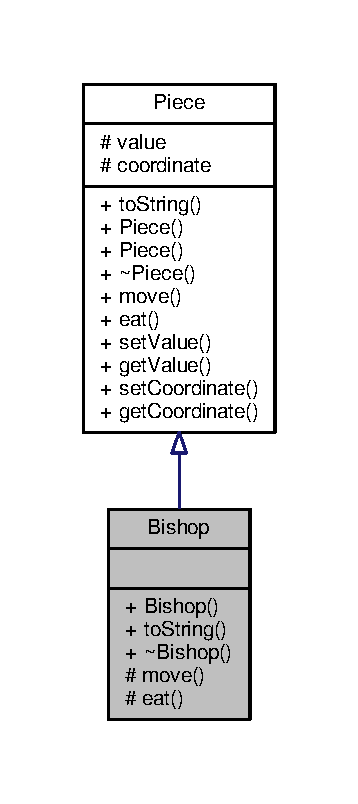
\includegraphics[width=172pt]{class_bishop__inherit__graph}
\end{center}
\end{figure}


Collaboration diagram for Bishop\+:\nopagebreak
\begin{figure}[H]
\begin{center}
\leavevmode
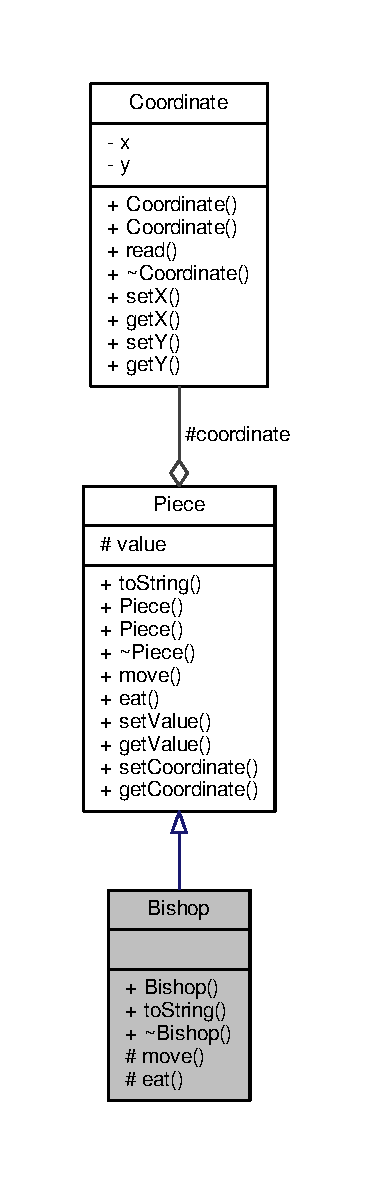
\includegraphics[height=550pt]{class_bishop__coll__graph}
\end{center}
\end{figure}
\subsection*{Public Member Functions}
\begin{DoxyCompactItemize}
\item 
\hyperlink{class_bishop_abc54c861677423ac25f0c819cb9cbb55}{Bishop} (\hyperlink{class_coordinate}{Coordinate} \hyperlink{class_piece_a9e92373c8fffc1f5efb20d62204b70cf}{coordinate})
\item 
virtual std\+::string \hyperlink{class_bishop_af69ba4eec8bcf5dad66c8071a168bdba}{to\+String} ()
\item 
virtual \hyperlink{class_bishop_a3705b4537a39d09a59143fe01a62442f}{$\sim$\+Bishop} ()
\end{DoxyCompactItemize}
\subsection*{Protected Member Functions}
\begin{DoxyCompactItemize}
\item 
virtual bool \hyperlink{class_bishop_afddd21905462db28e4f3f694d3f156df}{move} (\hyperlink{class_coordinate}{Coordinate} \hyperlink{class_piece_a9e92373c8fffc1f5efb20d62204b70cf}{coordinate}, \hyperlink{class_board}{Board} $\ast$board)
\item 
virtual bool \hyperlink{class_bishop_a2ff965d9d180e94989953544f0e9ae9b}{eat} (\hyperlink{class_coordinate}{Coordinate} \hyperlink{class_piece_a9e92373c8fffc1f5efb20d62204b70cf}{coordinate}, \hyperlink{class_board}{Board} $\ast$board)
\end{DoxyCompactItemize}
\subsection*{Additional Inherited Members}


\subsection{Detailed Description}
class \hyperlink{class_bishop}{Bishop} 

\subsection{Constructor \& Destructor Documentation}
\index{Bishop@{Bishop}!Bishop@{Bishop}}
\index{Bishop@{Bishop}!Bishop@{Bishop}}
\subsubsection[{\texorpdfstring{Bishop(\+Coordinate coordinate)}{Bishop(Coordinate coordinate)}}]{\setlength{\rightskip}{0pt plus 5cm}Bishop\+::\+Bishop (
\begin{DoxyParamCaption}
\item[{{\bf Coordinate}}]{coordinate}
\end{DoxyParamCaption}
)}\hypertarget{class_bishop_abc54c861677423ac25f0c819cb9cbb55}{}\label{class_bishop_abc54c861677423ac25f0c819cb9cbb55}
Empty Constructor \index{Bishop@{Bishop}!````~Bishop@{$\sim$\+Bishop}}
\index{````~Bishop@{$\sim$\+Bishop}!Bishop@{Bishop}}
\subsubsection[{\texorpdfstring{$\sim$\+Bishop()}{~Bishop()}}]{\setlength{\rightskip}{0pt plus 5cm}Bishop\+::$\sim$\+Bishop (
\begin{DoxyParamCaption}
{}
\end{DoxyParamCaption}
)\hspace{0.3cm}{\ttfamily [virtual]}}\hypertarget{class_bishop_a3705b4537a39d09a59143fe01a62442f}{}\label{class_bishop_a3705b4537a39d09a59143fe01a62442f}
Empty Destructor 

\subsection{Member Function Documentation}
\index{Bishop@{Bishop}!eat@{eat}}
\index{eat@{eat}!Bishop@{Bishop}}
\subsubsection[{\texorpdfstring{eat(\+Coordinate coordinate, Board $\ast$board)}{eat(Coordinate coordinate, Board *board)}}]{\setlength{\rightskip}{0pt plus 5cm}bool Bishop\+::eat (
\begin{DoxyParamCaption}
\item[{{\bf Coordinate}}]{coordinate, }
\item[{{\bf Board} $\ast$}]{board}
\end{DoxyParamCaption}
)\hspace{0.3cm}{\ttfamily [protected]}, {\ttfamily [virtual]}}\hypertarget{class_bishop_a2ff965d9d180e94989953544f0e9ae9b}{}\label{class_bishop_a2ff965d9d180e94989953544f0e9ae9b}


Implements \hyperlink{class_piece_a94fffb0c34e637910c08ded95185e135}{Piece}.

\index{Bishop@{Bishop}!move@{move}}
\index{move@{move}!Bishop@{Bishop}}
\subsubsection[{\texorpdfstring{move(\+Coordinate coordinate, Board $\ast$board)}{move(Coordinate coordinate, Board *board)}}]{\setlength{\rightskip}{0pt plus 5cm}bool Bishop\+::move (
\begin{DoxyParamCaption}
\item[{{\bf Coordinate}}]{coordinate, }
\item[{{\bf Board} $\ast$}]{board}
\end{DoxyParamCaption}
)\hspace{0.3cm}{\ttfamily [protected]}, {\ttfamily [virtual]}}\hypertarget{class_bishop_afddd21905462db28e4f3f694d3f156df}{}\label{class_bishop_afddd21905462db28e4f3f694d3f156df}


Implements \hyperlink{class_piece_a4939b8f41018950374d294b256906ec3}{Piece}.

\index{Bishop@{Bishop}!to\+String@{to\+String}}
\index{to\+String@{to\+String}!Bishop@{Bishop}}
\subsubsection[{\texorpdfstring{to\+String()}{toString()}}]{\setlength{\rightskip}{0pt plus 5cm}virtual std\+::string Bishop\+::to\+String (
\begin{DoxyParamCaption}
{}
\end{DoxyParamCaption}
)\hspace{0.3cm}{\ttfamily [inline]}, {\ttfamily [virtual]}}\hypertarget{class_bishop_af69ba4eec8bcf5dad66c8071a168bdba}{}\label{class_bishop_af69ba4eec8bcf5dad66c8071a168bdba}


Implements \hyperlink{class_piece_a2a017f933a49e17d9a60a665ee9df605}{Piece}.



The documentation for this class was generated from the following files\+:\begin{DoxyCompactItemize}
\item 
\hyperlink{_bishop_8h}{Bishop.\+h}\item 
\hyperlink{_bishop_8cpp}{Bishop.\+cpp}\end{DoxyCompactItemize}

\hypertarget{class_board}{}\section{Board Class Reference}
\label{class_board}\index{Board@{Board}}


{\ttfamily \#include $<$Board.\+h$>$}



Collaboration diagram for Board\+:\nopagebreak
\begin{figure}[H]
\begin{center}
\leavevmode
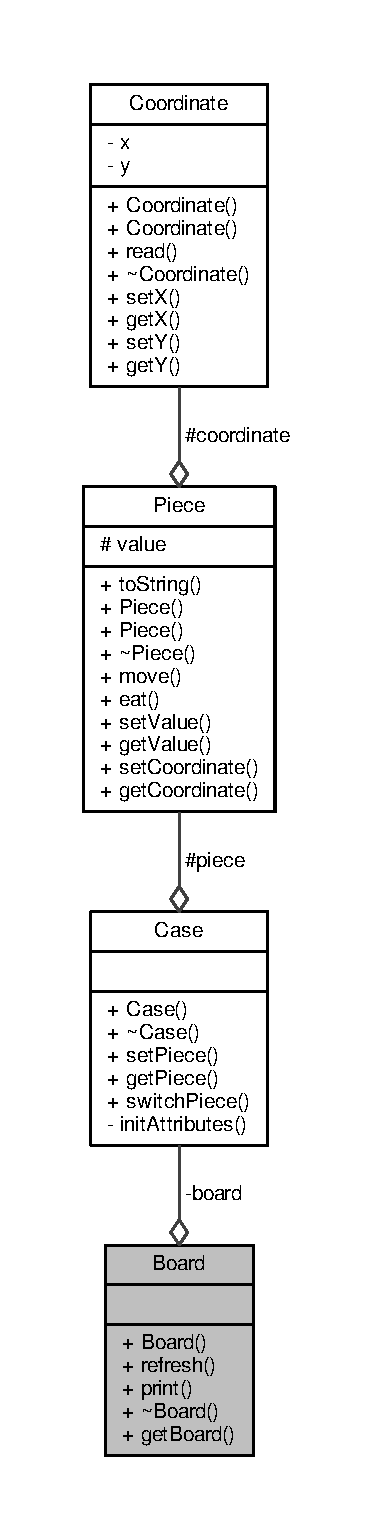
\includegraphics[height=550pt]{class_board__coll__graph}
\end{center}
\end{figure}
\subsection*{Public Member Functions}
\begin{DoxyCompactItemize}
\item 
\hyperlink{class_board_a9ee491d4fea680cf69b033374a9fdfcb}{Board} ()
\item 
void \hyperlink{class_board_a5ef838b8b50778bc0206d86204049eb0}{refresh} (\hyperlink{class_player}{Player} $\ast$player\+\_\+1, \hyperlink{class_player}{Player} $\ast$player\+\_\+2)
\item 
void \hyperlink{class_board_a93825eef8ed4d502861a855ae0610e21}{print} (\hyperlink{class_player}{Player} $\ast$player\+\_\+1, \hyperlink{class_player}{Player} $\ast$player\+\_\+2)
\item 
virtual \hyperlink{class_board_af73f45730119a1fd8f6670f53f959e68}{$\sim$\+Board} ()
\item 
\hyperlink{class_case}{Case} $\ast$$\ast$ \hyperlink{class_board_a701bcc81be3bab89830ce4f35016edcc}{get\+Board} ()
\end{DoxyCompactItemize}
\subsection*{Private Attributes}
\begin{DoxyCompactItemize}
\item 
\hyperlink{class_case}{Case} $\ast$$\ast$ \hyperlink{class_board_a4d7ad04642783accc669fccfae9a9727}{board}
\end{DoxyCompactItemize}


\subsection{Constructor \& Destructor Documentation}
\index{Board@{Board}!Board@{Board}}
\index{Board@{Board}!Board@{Board}}
\subsubsection[{\texorpdfstring{Board()}{Board()}}]{\setlength{\rightskip}{0pt plus 5cm}Board\+::\+Board (
\begin{DoxyParamCaption}
{}
\end{DoxyParamCaption}
)}\hypertarget{class_board_a9ee491d4fea680cf69b033374a9fdfcb}{}\label{class_board_a9ee491d4fea680cf69b033374a9fdfcb}
Empty Constructor \index{Board@{Board}!````~Board@{$\sim$\+Board}}
\index{````~Board@{$\sim$\+Board}!Board@{Board}}
\subsubsection[{\texorpdfstring{$\sim$\+Board()}{~Board()}}]{\setlength{\rightskip}{0pt plus 5cm}Board\+::$\sim$\+Board (
\begin{DoxyParamCaption}
{}
\end{DoxyParamCaption}
)\hspace{0.3cm}{\ttfamily [virtual]}}\hypertarget{class_board_af73f45730119a1fd8f6670f53f959e68}{}\label{class_board_af73f45730119a1fd8f6670f53f959e68}
Empty Destructor 

\subsection{Member Function Documentation}
\index{Board@{Board}!get\+Board@{get\+Board}}
\index{get\+Board@{get\+Board}!Board@{Board}}
\subsubsection[{\texorpdfstring{get\+Board()}{getBoard()}}]{\setlength{\rightskip}{0pt plus 5cm}{\bf Case}$\ast$$\ast$ Board\+::get\+Board (
\begin{DoxyParamCaption}
{}
\end{DoxyParamCaption}
)\hspace{0.3cm}{\ttfamily [inline]}}\hypertarget{class_board_a701bcc81be3bab89830ce4f35016edcc}{}\label{class_board_a701bcc81be3bab89830ce4f35016edcc}
Set the value of board 
\begin{DoxyParams}{Parameters}
{\em new\+\_\+var} & the new value of board Get the value of board \\
\hline
\end{DoxyParams}
\begin{DoxyReturn}{Returns}
the value of board 
\end{DoxyReturn}
\index{Board@{Board}!print@{print}}
\index{print@{print}!Board@{Board}}
\subsubsection[{\texorpdfstring{print(\+Player $\ast$player\+\_\+1, Player $\ast$player\+\_\+2)}{print(Player *player_1, Player *player_2)}}]{\setlength{\rightskip}{0pt plus 5cm}void Board\+::print (
\begin{DoxyParamCaption}
\item[{{\bf Player} $\ast$}]{player\+\_\+1, }
\item[{{\bf Player} $\ast$}]{player\+\_\+2}
\end{DoxyParamCaption}
)}\hypertarget{class_board_a93825eef8ed4d502861a855ae0610e21}{}\label{class_board_a93825eef8ed4d502861a855ae0610e21}
\index{Board@{Board}!refresh@{refresh}}
\index{refresh@{refresh}!Board@{Board}}
\subsubsection[{\texorpdfstring{refresh(\+Player $\ast$player\+\_\+1, Player $\ast$player\+\_\+2)}{refresh(Player *player_1, Player *player_2)}}]{\setlength{\rightskip}{0pt plus 5cm}void Board\+::refresh (
\begin{DoxyParamCaption}
\item[{{\bf Player} $\ast$}]{player\+\_\+1, }
\item[{{\bf Player} $\ast$}]{player\+\_\+2}
\end{DoxyParamCaption}
)}\hypertarget{class_board_a5ef838b8b50778bc0206d86204049eb0}{}\label{class_board_a5ef838b8b50778bc0206d86204049eb0}


\subsection{Member Data Documentation}
\index{Board@{Board}!board@{board}}
\index{board@{board}!Board@{Board}}
\subsubsection[{\texorpdfstring{board}{board}}]{\setlength{\rightskip}{0pt plus 5cm}{\bf Case}$\ast$$\ast$ Board\+::board\hspace{0.3cm}{\ttfamily [private]}}\hypertarget{class_board_a4d7ad04642783accc669fccfae9a9727}{}\label{class_board_a4d7ad04642783accc669fccfae9a9727}


The documentation for this class was generated from the following files\+:\begin{DoxyCompactItemize}
\item 
\hyperlink{_board_8h}{Board.\+h}\item 
\hyperlink{_board_8cpp}{Board.\+cpp}\end{DoxyCompactItemize}

\hypertarget{class_case}{}\section{Case Class Reference}
\label{class_case}\index{Case@{Case}}


{\ttfamily \#include $<$Case.\+h$>$}



Collaboration diagram for Case\+:
\nopagebreak
\begin{figure}[H]
\begin{center}
\leavevmode
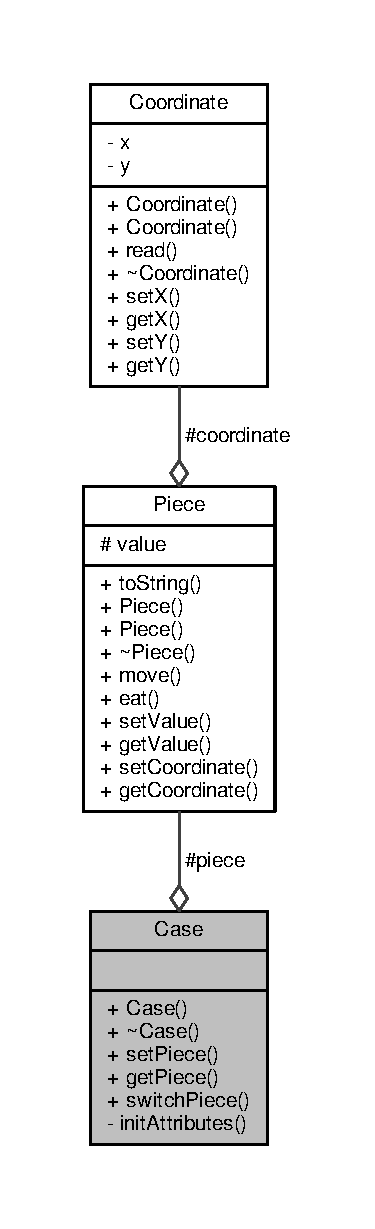
\includegraphics[height=550pt]{class_case__coll__graph}
\end{center}
\end{figure}
\subsection*{Public Member Functions}
\begin{DoxyCompactItemize}
\item 
\hyperlink{class_case_a14237e17aab1829965adab76b747db6c}{Case} ()
\item 
virtual \hyperlink{class_case_ab004564aae3e15db0c7fd5dde0b4c379}{$\sim$\+Case} ()
\item 
void \hyperlink{class_case_aaa0ce6e0cfcb0fc6bf38c7be1a82b1e0}{set\+Piece} (\hyperlink{class_piece}{Piece} $\ast$new\+\_\+var)
\item 
\hyperlink{class_piece}{Piece} $\ast$ \hyperlink{class_case_af7cd37da62062eb606a3b439e131c937}{get\+Piece} ()
\item 
void \hyperlink{class_case_a3a1a33aeb2401ff0f08dfb89b63832fa}{switch\+Piece} (\hyperlink{class_case}{Case} $\ast$case\+Two)
\end{DoxyCompactItemize}
\subsection*{Protected Attributes}
\begin{DoxyCompactItemize}
\item 
\hyperlink{class_piece}{Piece} $\ast$ \hyperlink{class_case_aecf7c05bfb4eaf8332f9c556319993a3}{piece}
\end{DoxyCompactItemize}
\subsection*{Private Member Functions}
\begin{DoxyCompactItemize}
\item 
void \hyperlink{class_case_a975dfe51150f130269224046566ee774}{init\+Attributes} ()
\end{DoxyCompactItemize}


\subsection{Detailed Description}
class \hyperlink{class_case}{Case} 

\subsection{Constructor \& Destructor Documentation}
\index{Case@{Case}!Case@{Case}}
\index{Case@{Case}!Case@{Case}}
\subsubsection[{\texorpdfstring{Case()}{Case()}}]{\setlength{\rightskip}{0pt plus 5cm}Case\+::\+Case (
\begin{DoxyParamCaption}
{}
\end{DoxyParamCaption}
)}\hypertarget{class_case_a14237e17aab1829965adab76b747db6c}{}\label{class_case_a14237e17aab1829965adab76b747db6c}
Empty Constructor \index{Case@{Case}!````~Case@{$\sim$\+Case}}
\index{````~Case@{$\sim$\+Case}!Case@{Case}}
\subsubsection[{\texorpdfstring{$\sim$\+Case()}{~Case()}}]{\setlength{\rightskip}{0pt plus 5cm}Case\+::$\sim$\+Case (
\begin{DoxyParamCaption}
{}
\end{DoxyParamCaption}
)\hspace{0.3cm}{\ttfamily [virtual]}}\hypertarget{class_case_ab004564aae3e15db0c7fd5dde0b4c379}{}\label{class_case_ab004564aae3e15db0c7fd5dde0b4c379}
Empty Destructor 

\subsection{Member Function Documentation}
\index{Case@{Case}!get\+Piece@{get\+Piece}}
\index{get\+Piece@{get\+Piece}!Case@{Case}}
\subsubsection[{\texorpdfstring{get\+Piece()}{getPiece()}}]{\setlength{\rightskip}{0pt plus 5cm}{\bf Piece}$\ast$ Case\+::get\+Piece (
\begin{DoxyParamCaption}
{}
\end{DoxyParamCaption}
)\hspace{0.3cm}{\ttfamily [inline]}}\hypertarget{class_case_af7cd37da62062eb606a3b439e131c937}{}\label{class_case_af7cd37da62062eb606a3b439e131c937}
Get the value of piece \begin{DoxyReturn}{Returns}
the value of piece 
\end{DoxyReturn}
\index{Case@{Case}!init\+Attributes@{init\+Attributes}}
\index{init\+Attributes@{init\+Attributes}!Case@{Case}}
\subsubsection[{\texorpdfstring{init\+Attributes()}{initAttributes()}}]{\setlength{\rightskip}{0pt plus 5cm}void Case\+::init\+Attributes (
\begin{DoxyParamCaption}
{}
\end{DoxyParamCaption}
)\hspace{0.3cm}{\ttfamily [private]}}\hypertarget{class_case_a975dfe51150f130269224046566ee774}{}\label{class_case_a975dfe51150f130269224046566ee774}
\index{Case@{Case}!set\+Piece@{set\+Piece}}
\index{set\+Piece@{set\+Piece}!Case@{Case}}
\subsubsection[{\texorpdfstring{set\+Piece(\+Piece $\ast$new\+\_\+var)}{setPiece(Piece *new_var)}}]{\setlength{\rightskip}{0pt plus 5cm}void Case\+::set\+Piece (
\begin{DoxyParamCaption}
\item[{{\bf Piece} $\ast$}]{new\+\_\+var}
\end{DoxyParamCaption}
)\hspace{0.3cm}{\ttfamily [inline]}}\hypertarget{class_case_aaa0ce6e0cfcb0fc6bf38c7be1a82b1e0}{}\label{class_case_aaa0ce6e0cfcb0fc6bf38c7be1a82b1e0}
Set the value of piece 
\begin{DoxyParams}{Parameters}
{\em new\+\_\+var} & the new value of piece \\
\hline
\end{DoxyParams}
\index{Case@{Case}!switch\+Piece@{switch\+Piece}}
\index{switch\+Piece@{switch\+Piece}!Case@{Case}}
\subsubsection[{\texorpdfstring{switch\+Piece(\+Case $\ast$case\+Two)}{switchPiece(Case *caseTwo)}}]{\setlength{\rightskip}{0pt plus 5cm}void Case\+::switch\+Piece (
\begin{DoxyParamCaption}
\item[{{\bf Case} $\ast$}]{case\+Two}
\end{DoxyParamCaption}
)}\hypertarget{class_case_a3a1a33aeb2401ff0f08dfb89b63832fa}{}\label{class_case_a3a1a33aeb2401ff0f08dfb89b63832fa}


\subsection{Member Data Documentation}
\index{Case@{Case}!piece@{piece}}
\index{piece@{piece}!Case@{Case}}
\subsubsection[{\texorpdfstring{piece}{piece}}]{\setlength{\rightskip}{0pt plus 5cm}{\bf Piece}$\ast$ Case\+::piece\hspace{0.3cm}{\ttfamily [protected]}}\hypertarget{class_case_aecf7c05bfb4eaf8332f9c556319993a3}{}\label{class_case_aecf7c05bfb4eaf8332f9c556319993a3}


The documentation for this class was generated from the following files\+:\begin{DoxyCompactItemize}
\item 
\hyperlink{_case_8h}{Case.\+h}\item 
\hyperlink{_case_8cpp}{Case.\+cpp}\end{DoxyCompactItemize}

\hypertarget{class_coordinate}{}\section{Coordinate Class Reference}
\label{class_coordinate}\index{Coordinate@{Coordinate}}


{\ttfamily \#include $<$Coordinate.\+h$>$}



Collaboration diagram for Coordinate\+:
\nopagebreak
\begin{figure}[H]
\begin{center}
\leavevmode
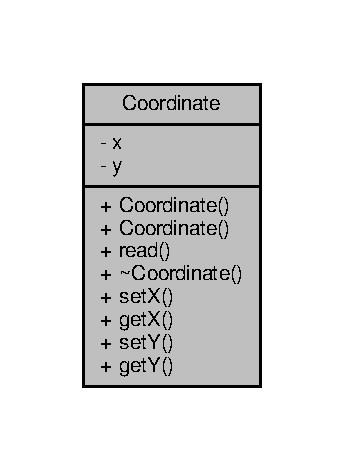
\includegraphics[width=165pt]{class_coordinate__coll__graph}
\end{center}
\end{figure}
\subsection*{Public Member Functions}
\begin{DoxyCompactItemize}
\item 
\hyperlink{class_coordinate_aac6f323a685fc1e88fbea9c86f1e600d}{Coordinate} ()
\item 
\hyperlink{class_coordinate_a8851ee18948f8b6433b0afc6b59095a7}{Coordinate} (unsigned int t\+\_\+x, unsigned int t\+\_\+y)
\item 
void \hyperlink{class_coordinate_a7a332d39b84136f15e8d3565b3c235f0}{read} ()
\item 
virtual \hyperlink{class_coordinate_ac57d6eb147832a234cc5deaff8c94346}{$\sim$\+Coordinate} ()
\item 
void \hyperlink{class_coordinate_a330c37af7bb87f30a55173617112eade}{setX} (unsigned int new\+\_\+var)
\item 
unsigned int \hyperlink{class_coordinate_a590d96a9210bc7c63854c88f8641dce8}{getX} ()
\item 
void \hyperlink{class_coordinate_ad4b804672ac33f50024d66f3bb46e033}{setY} (unsigned int new\+\_\+var)
\item 
unsigned int \hyperlink{class_coordinate_aafb7d8a5075196ba89e2cb8d70405a1c}{getY} ()
\end{DoxyCompactItemize}
\subsection*{Private Attributes}
\begin{DoxyCompactItemize}
\item 
unsigned int \hyperlink{class_coordinate_aed3fecfb15ebabe5b4905820c1999b0b}{x}
\item 
unsigned int \hyperlink{class_coordinate_a13eedbab9e112ef9f8685c12f1aed009}{y}
\end{DoxyCompactItemize}


\subsection{Detailed Description}
class \hyperlink{class_coordinate}{Coordinate} 

\subsection{Constructor \& Destructor Documentation}
\index{Coordinate@{Coordinate}!Coordinate@{Coordinate}}
\index{Coordinate@{Coordinate}!Coordinate@{Coordinate}}
\subsubsection[{\texorpdfstring{Coordinate()}{Coordinate()}}]{\setlength{\rightskip}{0pt plus 5cm}Coordinate\+::\+Coordinate (
\begin{DoxyParamCaption}
{}
\end{DoxyParamCaption}
)}\hypertarget{class_coordinate_aac6f323a685fc1e88fbea9c86f1e600d}{}\label{class_coordinate_aac6f323a685fc1e88fbea9c86f1e600d}
Empty Constructor \index{Coordinate@{Coordinate}!Coordinate@{Coordinate}}
\index{Coordinate@{Coordinate}!Coordinate@{Coordinate}}
\subsubsection[{\texorpdfstring{Coordinate(unsigned int t\+\_\+x, unsigned int t\+\_\+y)}{Coordinate(unsigned int t_x, unsigned int t_y)}}]{\setlength{\rightskip}{0pt plus 5cm}Coordinate\+::\+Coordinate (
\begin{DoxyParamCaption}
\item[{unsigned int}]{t\+\_\+x, }
\item[{unsigned int}]{t\+\_\+y}
\end{DoxyParamCaption}
)}\hypertarget{class_coordinate_a8851ee18948f8b6433b0afc6b59095a7}{}\label{class_coordinate_a8851ee18948f8b6433b0afc6b59095a7}
\index{Coordinate@{Coordinate}!````~Coordinate@{$\sim$\+Coordinate}}
\index{````~Coordinate@{$\sim$\+Coordinate}!Coordinate@{Coordinate}}
\subsubsection[{\texorpdfstring{$\sim$\+Coordinate()}{~Coordinate()}}]{\setlength{\rightskip}{0pt plus 5cm}Coordinate\+::$\sim$\+Coordinate (
\begin{DoxyParamCaption}
{}
\end{DoxyParamCaption}
)\hspace{0.3cm}{\ttfamily [virtual]}}\hypertarget{class_coordinate_ac57d6eb147832a234cc5deaff8c94346}{}\label{class_coordinate_ac57d6eb147832a234cc5deaff8c94346}
Empty Destructor 

\subsection{Member Function Documentation}
\index{Coordinate@{Coordinate}!getX@{getX}}
\index{getX@{getX}!Coordinate@{Coordinate}}
\subsubsection[{\texorpdfstring{get\+X()}{getX()}}]{\setlength{\rightskip}{0pt plus 5cm}unsigned int Coordinate\+::getX (
\begin{DoxyParamCaption}
{}
\end{DoxyParamCaption}
)\hspace{0.3cm}{\ttfamily [inline]}}\hypertarget{class_coordinate_a590d96a9210bc7c63854c88f8641dce8}{}\label{class_coordinate_a590d96a9210bc7c63854c88f8641dce8}
Get the value of x \begin{DoxyReturn}{Returns}
the value of x 
\end{DoxyReturn}
\index{Coordinate@{Coordinate}!getY@{getY}}
\index{getY@{getY}!Coordinate@{Coordinate}}
\subsubsection[{\texorpdfstring{get\+Y()}{getY()}}]{\setlength{\rightskip}{0pt plus 5cm}unsigned int Coordinate\+::getY (
\begin{DoxyParamCaption}
{}
\end{DoxyParamCaption}
)\hspace{0.3cm}{\ttfamily [inline]}}\hypertarget{class_coordinate_aafb7d8a5075196ba89e2cb8d70405a1c}{}\label{class_coordinate_aafb7d8a5075196ba89e2cb8d70405a1c}
Get the value of y \begin{DoxyReturn}{Returns}
the value of y 
\end{DoxyReturn}
\index{Coordinate@{Coordinate}!read@{read}}
\index{read@{read}!Coordinate@{Coordinate}}
\subsubsection[{\texorpdfstring{read()}{read()}}]{\setlength{\rightskip}{0pt plus 5cm}void Coordinate\+::read (
\begin{DoxyParamCaption}
{}
\end{DoxyParamCaption}
)}\hypertarget{class_coordinate_a7a332d39b84136f15e8d3565b3c235f0}{}\label{class_coordinate_a7a332d39b84136f15e8d3565b3c235f0}
\index{Coordinate@{Coordinate}!setX@{setX}}
\index{setX@{setX}!Coordinate@{Coordinate}}
\subsubsection[{\texorpdfstring{set\+X(unsigned int new\+\_\+var)}{setX(unsigned int new_var)}}]{\setlength{\rightskip}{0pt plus 5cm}void Coordinate\+::setX (
\begin{DoxyParamCaption}
\item[{unsigned int}]{new\+\_\+var}
\end{DoxyParamCaption}
)\hspace{0.3cm}{\ttfamily [inline]}}\hypertarget{class_coordinate_a330c37af7bb87f30a55173617112eade}{}\label{class_coordinate_a330c37af7bb87f30a55173617112eade}
Set the value of x 
\begin{DoxyParams}{Parameters}
{\em new\+\_\+var} & the new value of x \\
\hline
\end{DoxyParams}
\index{Coordinate@{Coordinate}!setY@{setY}}
\index{setY@{setY}!Coordinate@{Coordinate}}
\subsubsection[{\texorpdfstring{set\+Y(unsigned int new\+\_\+var)}{setY(unsigned int new_var)}}]{\setlength{\rightskip}{0pt plus 5cm}void Coordinate\+::setY (
\begin{DoxyParamCaption}
\item[{unsigned int}]{new\+\_\+var}
\end{DoxyParamCaption}
)\hspace{0.3cm}{\ttfamily [inline]}}\hypertarget{class_coordinate_ad4b804672ac33f50024d66f3bb46e033}{}\label{class_coordinate_ad4b804672ac33f50024d66f3bb46e033}
Set the value of y 
\begin{DoxyParams}{Parameters}
{\em new\+\_\+var} & the new value of y \\
\hline
\end{DoxyParams}


\subsection{Member Data Documentation}
\index{Coordinate@{Coordinate}!x@{x}}
\index{x@{x}!Coordinate@{Coordinate}}
\subsubsection[{\texorpdfstring{x}{x}}]{\setlength{\rightskip}{0pt plus 5cm}unsigned int Coordinate\+::x\hspace{0.3cm}{\ttfamily [private]}}\hypertarget{class_coordinate_aed3fecfb15ebabe5b4905820c1999b0b}{}\label{class_coordinate_aed3fecfb15ebabe5b4905820c1999b0b}
\index{Coordinate@{Coordinate}!y@{y}}
\index{y@{y}!Coordinate@{Coordinate}}
\subsubsection[{\texorpdfstring{y}{y}}]{\setlength{\rightskip}{0pt plus 5cm}unsigned int Coordinate\+::y\hspace{0.3cm}{\ttfamily [private]}}\hypertarget{class_coordinate_a13eedbab9e112ef9f8685c12f1aed009}{}\label{class_coordinate_a13eedbab9e112ef9f8685c12f1aed009}


The documentation for this class was generated from the following files\+:\begin{DoxyCompactItemize}
\item 
\hyperlink{_coordinate_8h}{Coordinate.\+h}\item 
\hyperlink{_coordinate_8cpp}{Coordinate.\+cpp}\end{DoxyCompactItemize}

\hypertarget{class_game}{}\section{Game Class Reference}
\label{class_game}\index{Game@{Game}}


{\ttfamily \#include $<$Game.\+h$>$}



Collaboration diagram for Game\+:\nopagebreak
\begin{figure}[H]
\begin{center}
\leavevmode
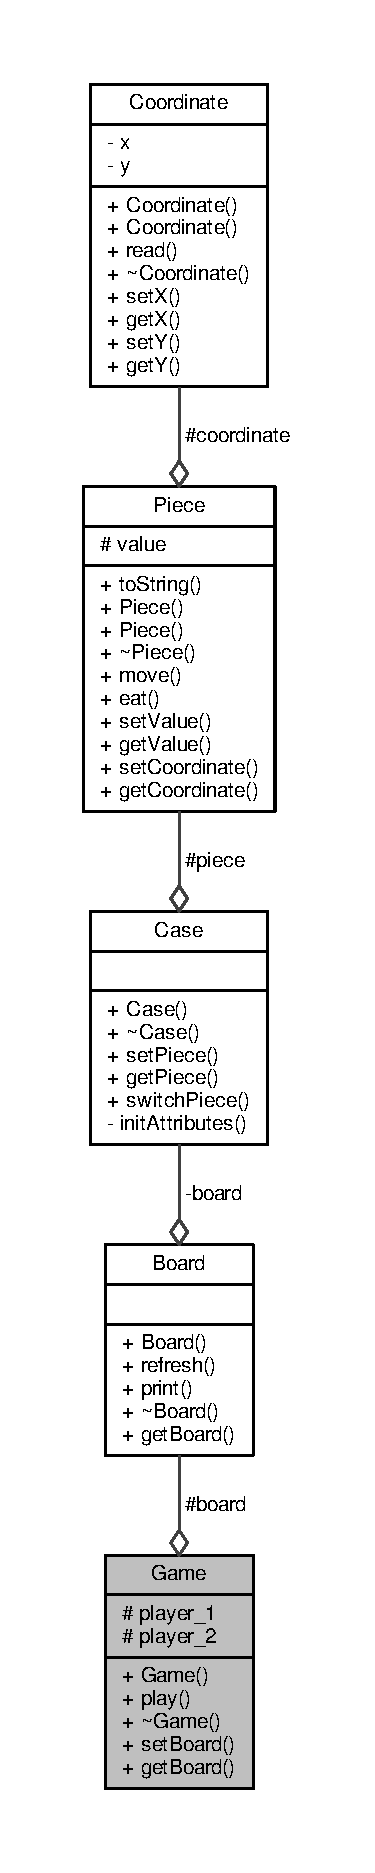
\includegraphics[height=550pt]{class_game__coll__graph}
\end{center}
\end{figure}
\subsection*{Public Member Functions}
\begin{DoxyCompactItemize}
\item 
\hyperlink{class_game_ad59df6562a58a614fda24622d3715b65}{Game} ()
\item 
bool \hyperlink{class_game_a42caf1acd21c76c606796caa7309c81a}{play} ()
\item 
virtual \hyperlink{class_game_ae3d112ca6e0e55150d2fdbc704474530}{$\sim$\+Game} ()
\item 
void \hyperlink{class_game_a972198b713c8d23acf06c0e95cc1c872}{set\+Board} (\hyperlink{class_board}{Board} $\ast$new\+\_\+var)
\item 
\hyperlink{class_board}{Board} $\ast$ \hyperlink{class_game_af886b92851f6e39dae9c88c8c2a84dda}{get\+Board} ()
\end{DoxyCompactItemize}
\subsection*{Protected Attributes}
\begin{DoxyCompactItemize}
\item 
\hyperlink{class_board}{Board} $\ast$ \hyperlink{class_game_ae38e501e177586af48d2e2300b6be4ba}{board}
\item 
std\+::list$<$ \hyperlink{class_player}{Player} $\ast$ $>$ \hyperlink{class_game_a093479c41ed1861885680ced9338b25e}{player\+\_\+1}
\item 
std\+::list$<$ \hyperlink{class_player}{Player} $\ast$ $>$ \hyperlink{class_game_a2146316babdcda94567af75f94b73106}{player\+\_\+2}
\end{DoxyCompactItemize}


\subsection{Detailed Description}
class \hyperlink{class_game}{Game} 

\subsection{Constructor \& Destructor Documentation}
\index{Game@{Game}!Game@{Game}}
\index{Game@{Game}!Game@{Game}}
\subsubsection[{\texorpdfstring{Game()}{Game()}}]{\setlength{\rightskip}{0pt plus 5cm}Game\+::\+Game (
\begin{DoxyParamCaption}
{}
\end{DoxyParamCaption}
)}\hypertarget{class_game_ad59df6562a58a614fda24622d3715b65}{}\label{class_game_ad59df6562a58a614fda24622d3715b65}
Empty Constructor \index{Game@{Game}!````~Game@{$\sim$\+Game}}
\index{````~Game@{$\sim$\+Game}!Game@{Game}}
\subsubsection[{\texorpdfstring{$\sim$\+Game()}{~Game()}}]{\setlength{\rightskip}{0pt plus 5cm}Game\+::$\sim$\+Game (
\begin{DoxyParamCaption}
{}
\end{DoxyParamCaption}
)\hspace{0.3cm}{\ttfamily [virtual]}}\hypertarget{class_game_ae3d112ca6e0e55150d2fdbc704474530}{}\label{class_game_ae3d112ca6e0e55150d2fdbc704474530}
Empty Destructor 

\subsection{Member Function Documentation}
\index{Game@{Game}!get\+Board@{get\+Board}}
\index{get\+Board@{get\+Board}!Game@{Game}}
\subsubsection[{\texorpdfstring{get\+Board()}{getBoard()}}]{\setlength{\rightskip}{0pt plus 5cm}{\bf Board}$\ast$ Game\+::get\+Board (
\begin{DoxyParamCaption}
{}
\end{DoxyParamCaption}
)\hspace{0.3cm}{\ttfamily [inline]}}\hypertarget{class_game_af886b92851f6e39dae9c88c8c2a84dda}{}\label{class_game_af886b92851f6e39dae9c88c8c2a84dda}
Get the value of board \begin{DoxyReturn}{Returns}
the value of board 
\end{DoxyReturn}
\index{Game@{Game}!play@{play}}
\index{play@{play}!Game@{Game}}
\subsubsection[{\texorpdfstring{play()}{play()}}]{\setlength{\rightskip}{0pt plus 5cm}bool Game\+::play (
\begin{DoxyParamCaption}
{}
\end{DoxyParamCaption}
)}\hypertarget{class_game_a42caf1acd21c76c606796caa7309c81a}{}\label{class_game_a42caf1acd21c76c606796caa7309c81a}
\index{Game@{Game}!set\+Board@{set\+Board}}
\index{set\+Board@{set\+Board}!Game@{Game}}
\subsubsection[{\texorpdfstring{set\+Board(\+Board $\ast$new\+\_\+var)}{setBoard(Board *new_var)}}]{\setlength{\rightskip}{0pt plus 5cm}void Game\+::set\+Board (
\begin{DoxyParamCaption}
\item[{{\bf Board} $\ast$}]{new\+\_\+var}
\end{DoxyParamCaption}
)\hspace{0.3cm}{\ttfamily [inline]}}\hypertarget{class_game_a972198b713c8d23acf06c0e95cc1c872}{}\label{class_game_a972198b713c8d23acf06c0e95cc1c872}
Set the value of board 
\begin{DoxyParams}{Parameters}
{\em new\+\_\+var} & the new value of board \\
\hline
\end{DoxyParams}


\subsection{Member Data Documentation}
\index{Game@{Game}!board@{board}}
\index{board@{board}!Game@{Game}}
\subsubsection[{\texorpdfstring{board}{board}}]{\setlength{\rightskip}{0pt plus 5cm}{\bf Board}$\ast$ Game\+::board\hspace{0.3cm}{\ttfamily [protected]}}\hypertarget{class_game_ae38e501e177586af48d2e2300b6be4ba}{}\label{class_game_ae38e501e177586af48d2e2300b6be4ba}
\index{Game@{Game}!player\+\_\+1@{player\+\_\+1}}
\index{player\+\_\+1@{player\+\_\+1}!Game@{Game}}
\subsubsection[{\texorpdfstring{player\+\_\+1}{player_1}}]{\setlength{\rightskip}{0pt plus 5cm}std\+::list$<${\bf Player} $\ast$$>$ Game\+::player\+\_\+1\hspace{0.3cm}{\ttfamily [protected]}}\hypertarget{class_game_a093479c41ed1861885680ced9338b25e}{}\label{class_game_a093479c41ed1861885680ced9338b25e}
\index{Game@{Game}!player\+\_\+2@{player\+\_\+2}}
\index{player\+\_\+2@{player\+\_\+2}!Game@{Game}}
\subsubsection[{\texorpdfstring{player\+\_\+2}{player_2}}]{\setlength{\rightskip}{0pt plus 5cm}std\+::list$<${\bf Player} $\ast$$>$ Game\+::player\+\_\+2\hspace{0.3cm}{\ttfamily [protected]}}\hypertarget{class_game_a2146316babdcda94567af75f94b73106}{}\label{class_game_a2146316babdcda94567af75f94b73106}


The documentation for this class was generated from the following files\+:\begin{DoxyCompactItemize}
\item 
\hyperlink{_game_8h}{Game.\+h}\item 
\hyperlink{_game_8cpp}{Game.\+cpp}\end{DoxyCompactItemize}

\hypertarget{class_king}{}\section{King Class Reference}
\label{class_king}\index{King@{King}}


{\ttfamily \#include $<$King.\+h$>$}



Inheritance diagram for King\+:\nopagebreak
\begin{figure}[H]
\begin{center}
\leavevmode
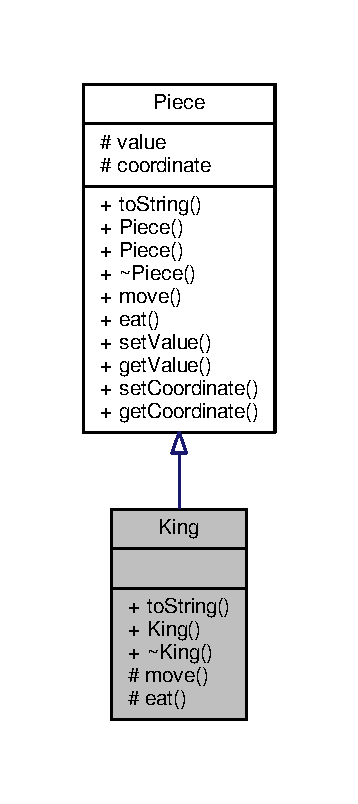
\includegraphics[width=172pt]{class_king__inherit__graph}
\end{center}
\end{figure}


Collaboration diagram for King\+:\nopagebreak
\begin{figure}[H]
\begin{center}
\leavevmode
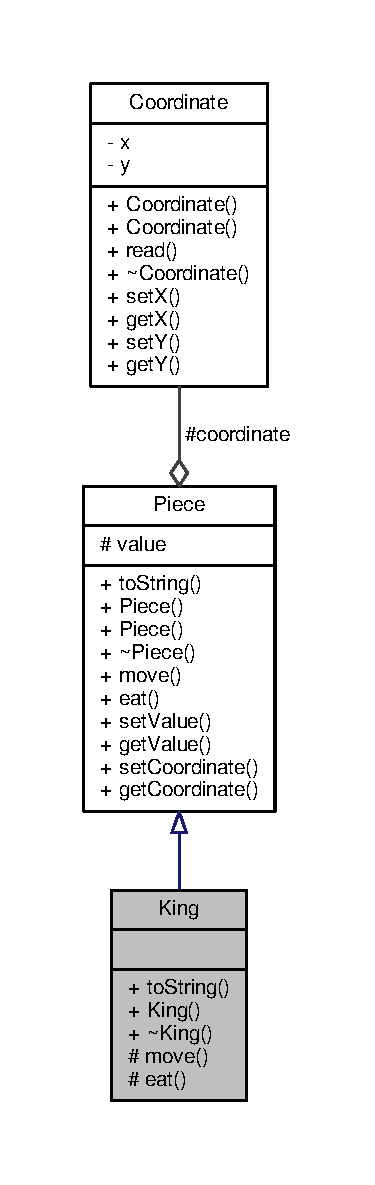
\includegraphics[height=550pt]{class_king__coll__graph}
\end{center}
\end{figure}
\subsection*{Public Member Functions}
\begin{DoxyCompactItemize}
\item 
virtual std\+::string \hyperlink{class_king_a445fa11a84a95f5257eea4fb0a4f4839}{to\+String} ()
\item 
\hyperlink{class_king_a61f66f3da9c9b8cda2541fb3e1be8743}{King} (\hyperlink{class_coordinate}{Coordinate} \hyperlink{class_piece_a9e92373c8fffc1f5efb20d62204b70cf}{coordinate})
\item 
virtual \hyperlink{class_king_aac368ce96e2b12f62e3608d27262e941}{$\sim$\+King} ()
\end{DoxyCompactItemize}
\subsection*{Protected Member Functions}
\begin{DoxyCompactItemize}
\item 
virtual bool \hyperlink{class_king_ac9319f67056661e2cf0abe05a78407ee}{move} (\hyperlink{class_coordinate}{Coordinate} \hyperlink{class_piece_a9e92373c8fffc1f5efb20d62204b70cf}{coordinate}, \hyperlink{class_board}{Board} $\ast$board)
\item 
virtual bool \hyperlink{class_king_abd8a9ef79a3a139afa83c2814edc852e}{eat} (\hyperlink{class_coordinate}{Coordinate} \hyperlink{class_piece_a9e92373c8fffc1f5efb20d62204b70cf}{coordinate}, \hyperlink{class_board}{Board} $\ast$board)
\end{DoxyCompactItemize}
\subsection*{Additional Inherited Members}


\subsection{Detailed Description}
class \hyperlink{class_king}{King} 

\subsection{Constructor \& Destructor Documentation}
\index{King@{King}!King@{King}}
\index{King@{King}!King@{King}}
\subsubsection[{\texorpdfstring{King(\+Coordinate coordinate)}{King(Coordinate coordinate)}}]{\setlength{\rightskip}{0pt plus 5cm}King\+::\+King (
\begin{DoxyParamCaption}
\item[{{\bf Coordinate}}]{coordinate}
\end{DoxyParamCaption}
)}\hypertarget{class_king_a61f66f3da9c9b8cda2541fb3e1be8743}{}\label{class_king_a61f66f3da9c9b8cda2541fb3e1be8743}
Empty Constructor \index{King@{King}!````~King@{$\sim$\+King}}
\index{````~King@{$\sim$\+King}!King@{King}}
\subsubsection[{\texorpdfstring{$\sim$\+King()}{~King()}}]{\setlength{\rightskip}{0pt plus 5cm}King\+::$\sim$\+King (
\begin{DoxyParamCaption}
{}
\end{DoxyParamCaption}
)\hspace{0.3cm}{\ttfamily [virtual]}}\hypertarget{class_king_aac368ce96e2b12f62e3608d27262e941}{}\label{class_king_aac368ce96e2b12f62e3608d27262e941}
Empty Destructor 

\subsection{Member Function Documentation}
\index{King@{King}!eat@{eat}}
\index{eat@{eat}!King@{King}}
\subsubsection[{\texorpdfstring{eat(\+Coordinate coordinate, Board $\ast$board)}{eat(Coordinate coordinate, Board *board)}}]{\setlength{\rightskip}{0pt plus 5cm}bool King\+::eat (
\begin{DoxyParamCaption}
\item[{{\bf Coordinate}}]{coordinate, }
\item[{{\bf Board} $\ast$}]{board}
\end{DoxyParamCaption}
)\hspace{0.3cm}{\ttfamily [protected]}, {\ttfamily [virtual]}}\hypertarget{class_king_abd8a9ef79a3a139afa83c2814edc852e}{}\label{class_king_abd8a9ef79a3a139afa83c2814edc852e}


Implements \hyperlink{class_piece_a94fffb0c34e637910c08ded95185e135}{Piece}.

\index{King@{King}!move@{move}}
\index{move@{move}!King@{King}}
\subsubsection[{\texorpdfstring{move(\+Coordinate coordinate, Board $\ast$board)}{move(Coordinate coordinate, Board *board)}}]{\setlength{\rightskip}{0pt plus 5cm}bool King\+::move (
\begin{DoxyParamCaption}
\item[{{\bf Coordinate}}]{coordinate, }
\item[{{\bf Board} $\ast$}]{board}
\end{DoxyParamCaption}
)\hspace{0.3cm}{\ttfamily [protected]}, {\ttfamily [virtual]}}\hypertarget{class_king_ac9319f67056661e2cf0abe05a78407ee}{}\label{class_king_ac9319f67056661e2cf0abe05a78407ee}


Implements \hyperlink{class_piece_a4939b8f41018950374d294b256906ec3}{Piece}.

\index{King@{King}!to\+String@{to\+String}}
\index{to\+String@{to\+String}!King@{King}}
\subsubsection[{\texorpdfstring{to\+String()}{toString()}}]{\setlength{\rightskip}{0pt plus 5cm}virtual std\+::string King\+::to\+String (
\begin{DoxyParamCaption}
{}
\end{DoxyParamCaption}
)\hspace{0.3cm}{\ttfamily [inline]}, {\ttfamily [virtual]}}\hypertarget{class_king_a445fa11a84a95f5257eea4fb0a4f4839}{}\label{class_king_a445fa11a84a95f5257eea4fb0a4f4839}


Implements \hyperlink{class_piece_a2a017f933a49e17d9a60a665ee9df605}{Piece}.



The documentation for this class was generated from the following files\+:\begin{DoxyCompactItemize}
\item 
\hyperlink{_king_8h}{King.\+h}\item 
\hyperlink{_king_8cpp}{King.\+cpp}\end{DoxyCompactItemize}

\hypertarget{class_knight}{}\section{Knight Class Reference}
\label{class_knight}\index{Knight@{Knight}}


{\ttfamily \#include $<$Knight.\+h$>$}



Inheritance diagram for Knight\+:\nopagebreak
\begin{figure}[H]
\begin{center}
\leavevmode
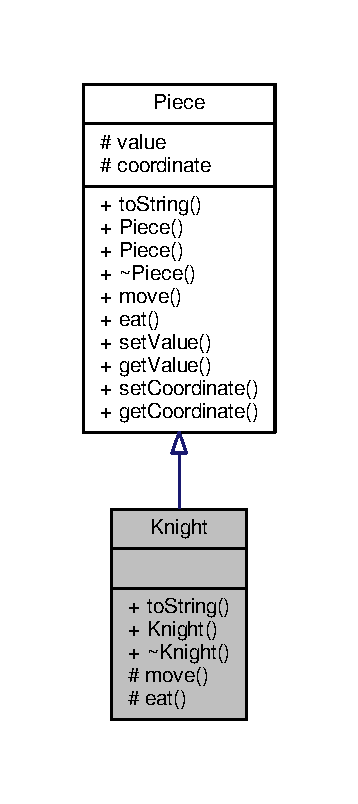
\includegraphics[width=172pt]{class_knight__inherit__graph}
\end{center}
\end{figure}


Collaboration diagram for Knight\+:\nopagebreak
\begin{figure}[H]
\begin{center}
\leavevmode
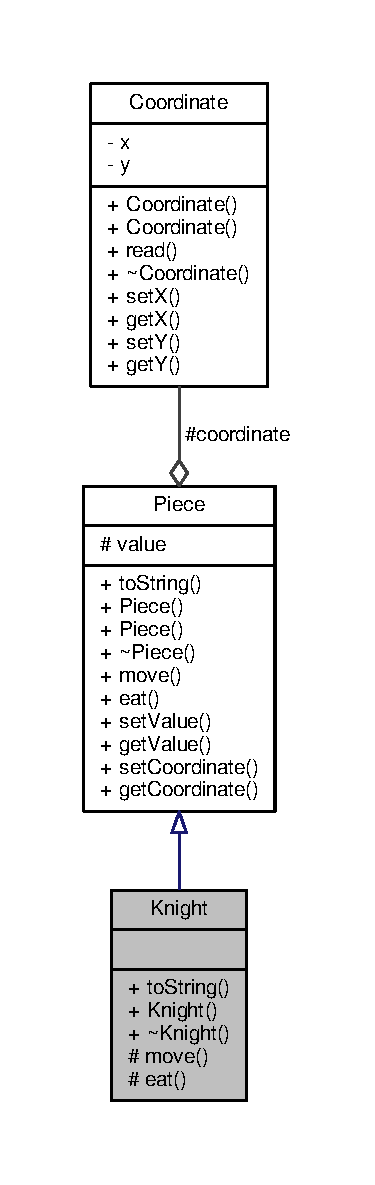
\includegraphics[height=550pt]{class_knight__coll__graph}
\end{center}
\end{figure}
\subsection*{Public Member Functions}
\begin{DoxyCompactItemize}
\item 
virtual std\+::string \hyperlink{class_knight_a3ecdeb255fa07eaa22d0cc948520c181}{to\+String} ()
\item 
\hyperlink{class_knight_ada9451f9c4ae0b30e7c0f0eaa7c78aac}{Knight} (\hyperlink{class_coordinate}{Coordinate} \hyperlink{class_piece_a9e92373c8fffc1f5efb20d62204b70cf}{coordinate})
\item 
virtual \hyperlink{class_knight_a2754123d6876babe915f4da8f761361b}{$\sim$\+Knight} ()
\end{DoxyCompactItemize}
\subsection*{Protected Member Functions}
\begin{DoxyCompactItemize}
\item 
virtual bool \hyperlink{class_knight_a852359fbd2d2d5e00445d07c3ec6fdfe}{move} (\hyperlink{class_coordinate}{Coordinate} \hyperlink{class_piece_a9e92373c8fffc1f5efb20d62204b70cf}{coordinate}, \hyperlink{class_board}{Board} $\ast$board)
\item 
virtual bool \hyperlink{class_knight_a5f92f60471d409e3afddefd760d993ec}{eat} (\hyperlink{class_coordinate}{Coordinate} \hyperlink{class_piece_a9e92373c8fffc1f5efb20d62204b70cf}{coordinate}, \hyperlink{class_board}{Board} $\ast$board)
\end{DoxyCompactItemize}
\subsection*{Additional Inherited Members}


\subsection{Detailed Description}
class \hyperlink{class_knight}{Knight} 

\subsection{Constructor \& Destructor Documentation}
\index{Knight@{Knight}!Knight@{Knight}}
\index{Knight@{Knight}!Knight@{Knight}}
\subsubsection[{\texorpdfstring{Knight(\+Coordinate coordinate)}{Knight(Coordinate coordinate)}}]{\setlength{\rightskip}{0pt plus 5cm}Knight\+::\+Knight (
\begin{DoxyParamCaption}
\item[{{\bf Coordinate}}]{coordinate}
\end{DoxyParamCaption}
)}\hypertarget{class_knight_ada9451f9c4ae0b30e7c0f0eaa7c78aac}{}\label{class_knight_ada9451f9c4ae0b30e7c0f0eaa7c78aac}
Empty Constructor \index{Knight@{Knight}!````~Knight@{$\sim$\+Knight}}
\index{````~Knight@{$\sim$\+Knight}!Knight@{Knight}}
\subsubsection[{\texorpdfstring{$\sim$\+Knight()}{~Knight()}}]{\setlength{\rightskip}{0pt plus 5cm}Knight\+::$\sim$\+Knight (
\begin{DoxyParamCaption}
{}
\end{DoxyParamCaption}
)\hspace{0.3cm}{\ttfamily [virtual]}}\hypertarget{class_knight_a2754123d6876babe915f4da8f761361b}{}\label{class_knight_a2754123d6876babe915f4da8f761361b}
Empty Destructor 

\subsection{Member Function Documentation}
\index{Knight@{Knight}!eat@{eat}}
\index{eat@{eat}!Knight@{Knight}}
\subsubsection[{\texorpdfstring{eat(\+Coordinate coordinate, Board $\ast$board)}{eat(Coordinate coordinate, Board *board)}}]{\setlength{\rightskip}{0pt plus 5cm}bool Knight\+::eat (
\begin{DoxyParamCaption}
\item[{{\bf Coordinate}}]{coordinate, }
\item[{{\bf Board} $\ast$}]{board}
\end{DoxyParamCaption}
)\hspace{0.3cm}{\ttfamily [protected]}, {\ttfamily [virtual]}}\hypertarget{class_knight_a5f92f60471d409e3afddefd760d993ec}{}\label{class_knight_a5f92f60471d409e3afddefd760d993ec}


Implements \hyperlink{class_piece_a94fffb0c34e637910c08ded95185e135}{Piece}.

\index{Knight@{Knight}!move@{move}}
\index{move@{move}!Knight@{Knight}}
\subsubsection[{\texorpdfstring{move(\+Coordinate coordinate, Board $\ast$board)}{move(Coordinate coordinate, Board *board)}}]{\setlength{\rightskip}{0pt plus 5cm}bool Knight\+::move (
\begin{DoxyParamCaption}
\item[{{\bf Coordinate}}]{coordinate, }
\item[{{\bf Board} $\ast$}]{board}
\end{DoxyParamCaption}
)\hspace{0.3cm}{\ttfamily [protected]}, {\ttfamily [virtual]}}\hypertarget{class_knight_a852359fbd2d2d5e00445d07c3ec6fdfe}{}\label{class_knight_a852359fbd2d2d5e00445d07c3ec6fdfe}


Implements \hyperlink{class_piece_a4939b8f41018950374d294b256906ec3}{Piece}.

\index{Knight@{Knight}!to\+String@{to\+String}}
\index{to\+String@{to\+String}!Knight@{Knight}}
\subsubsection[{\texorpdfstring{to\+String()}{toString()}}]{\setlength{\rightskip}{0pt plus 5cm}virtual std\+::string Knight\+::to\+String (
\begin{DoxyParamCaption}
{}
\end{DoxyParamCaption}
)\hspace{0.3cm}{\ttfamily [inline]}, {\ttfamily [virtual]}}\hypertarget{class_knight_a3ecdeb255fa07eaa22d0cc948520c181}{}\label{class_knight_a3ecdeb255fa07eaa22d0cc948520c181}


Implements \hyperlink{class_piece_a2a017f933a49e17d9a60a665ee9df605}{Piece}.



The documentation for this class was generated from the following files\+:\begin{DoxyCompactItemize}
\item 
\hyperlink{_knight_8h}{Knight.\+h}\item 
\hyperlink{_knight_8cpp}{Knight.\+cpp}\end{DoxyCompactItemize}

\hypertarget{class_memento_game}{}\section{Memento\+Game Class Reference}
\label{class_memento_game}\index{Memento\+Game@{Memento\+Game}}


{\ttfamily \#include $<$Memento\+Game.\+h$>$}



Collaboration diagram for Memento\+Game\+:
\nopagebreak
\begin{figure}[H]
\begin{center}
\leavevmode
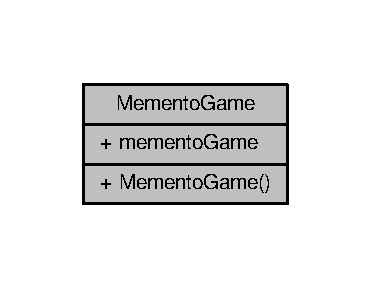
\includegraphics[width=178pt]{class_memento_game__coll__graph}
\end{center}
\end{figure}
\subsection*{Public Member Functions}
\begin{DoxyCompactItemize}
\item 
\hyperlink{class_memento_game_a2993ec1d28cf09c727935f0a274998b7}{Memento\+Game} ()
\end{DoxyCompactItemize}
\subsection*{Public Attributes}
\begin{DoxyCompactItemize}
\item 
std\+::list$<$ \hyperlink{class_game}{Game} $>$ \hyperlink{class_memento_game_ab6e7ce49855575ec2b963c452cc5ddc2}{memento\+Game}
\end{DoxyCompactItemize}
\subsection*{Friends}
\begin{DoxyCompactItemize}
\item 
class \hyperlink{class_memento_game_aa2fab026580d6f14280c2ffb8063a314}{Game}
\end{DoxyCompactItemize}


\subsection{Constructor \& Destructor Documentation}
\index{Memento\+Game@{Memento\+Game}!Memento\+Game@{Memento\+Game}}
\index{Memento\+Game@{Memento\+Game}!Memento\+Game@{Memento\+Game}}
\subsubsection[{\texorpdfstring{Memento\+Game()}{MementoGame()}}]{\setlength{\rightskip}{0pt plus 5cm}Memento\+Game\+::\+Memento\+Game (
\begin{DoxyParamCaption}
{}
\end{DoxyParamCaption}
)}\hypertarget{class_memento_game_a2993ec1d28cf09c727935f0a274998b7}{}\label{class_memento_game_a2993ec1d28cf09c727935f0a274998b7}


\subsection{Friends And Related Function Documentation}
\index{Memento\+Game@{Memento\+Game}!Game@{Game}}
\index{Game@{Game}!Memento\+Game@{Memento\+Game}}
\subsubsection[{\texorpdfstring{Game}{Game}}]{\setlength{\rightskip}{0pt plus 5cm}friend class {\bf Game}\hspace{0.3cm}{\ttfamily [friend]}}\hypertarget{class_memento_game_aa2fab026580d6f14280c2ffb8063a314}{}\label{class_memento_game_aa2fab026580d6f14280c2ffb8063a314}


\subsection{Member Data Documentation}
\index{Memento\+Game@{Memento\+Game}!memento\+Game@{memento\+Game}}
\index{memento\+Game@{memento\+Game}!Memento\+Game@{Memento\+Game}}
\subsubsection[{\texorpdfstring{memento\+Game}{mementoGame}}]{\setlength{\rightskip}{0pt plus 5cm}std\+::list$<${\bf Game}$>$ Memento\+Game\+::memento\+Game}\hypertarget{class_memento_game_ab6e7ce49855575ec2b963c452cc5ddc2}{}\label{class_memento_game_ab6e7ce49855575ec2b963c452cc5ddc2}


The documentation for this class was generated from the following files\+:\begin{DoxyCompactItemize}
\item 
\hyperlink{_memento_game_8h}{Memento\+Game.\+h}\item 
\hyperlink{_memento_game_8cpp}{Memento\+Game.\+cpp}\end{DoxyCompactItemize}

\hypertarget{class_pawn}{}\section{Pawn Class Reference}
\label{class_pawn}\index{Pawn@{Pawn}}


{\ttfamily \#include $<$Pawn.\+h$>$}



Inheritance diagram for Pawn\+:\nopagebreak
\begin{figure}[H]
\begin{center}
\leavevmode
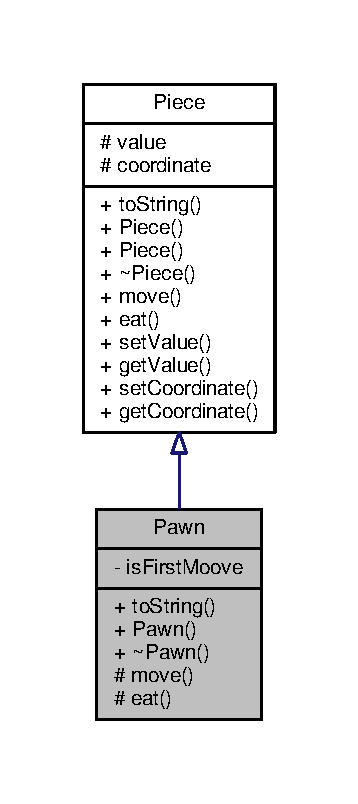
\includegraphics[width=172pt]{class_pawn__inherit__graph}
\end{center}
\end{figure}


Collaboration diagram for Pawn\+:\nopagebreak
\begin{figure}[H]
\begin{center}
\leavevmode
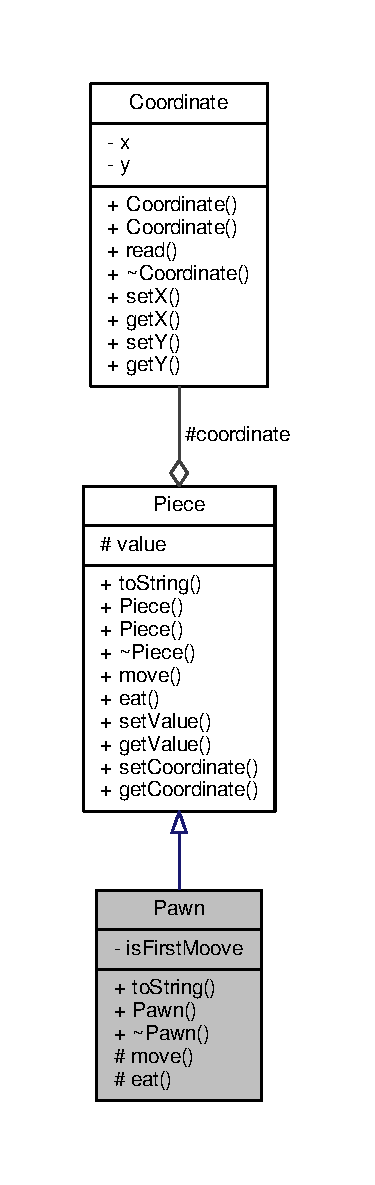
\includegraphics[height=550pt]{class_pawn__coll__graph}
\end{center}
\end{figure}
\subsection*{Public Member Functions}
\begin{DoxyCompactItemize}
\item 
virtual std\+::string \hyperlink{class_pawn_afac4abaf92106777e20d21fde635ffc4}{to\+String} ()
\item 
\hyperlink{class_pawn_a28054ee4fa72e69892be4d250191aa22}{Pawn} (\hyperlink{class_coordinate}{Coordinate} \hyperlink{class_piece_a9e92373c8fffc1f5efb20d62204b70cf}{coordinate})
\item 
virtual \hyperlink{class_pawn_a3095938fb8326469c3bd05da0b8f50af}{$\sim$\+Pawn} ()
\end{DoxyCompactItemize}
\subsection*{Protected Member Functions}
\begin{DoxyCompactItemize}
\item 
virtual bool \hyperlink{class_pawn_ae5ac3a2e71798fc8b6226bb9590497ea}{move} (\hyperlink{class_coordinate}{Coordinate} \hyperlink{class_piece_a9e92373c8fffc1f5efb20d62204b70cf}{coordinate}, \hyperlink{class_board}{Board} $\ast$board)
\item 
virtual bool \hyperlink{class_pawn_a3a6fd81c625f8df7d2ae90520c0937fe}{eat} (\hyperlink{class_coordinate}{Coordinate} \hyperlink{class_piece_a9e92373c8fffc1f5efb20d62204b70cf}{coordinate}, \hyperlink{class_board}{Board} $\ast$board)
\end{DoxyCompactItemize}
\subsection*{Private Attributes}
\begin{DoxyCompactItemize}
\item 
bool \hyperlink{class_pawn_abf900800320dfe79093b50baeda255d4}{is\+First\+Moove}
\end{DoxyCompactItemize}
\subsection*{Additional Inherited Members}


\subsection{Detailed Description}
class \hyperlink{class_pawn}{Pawn} 

\subsection{Constructor \& Destructor Documentation}
\index{Pawn@{Pawn}!Pawn@{Pawn}}
\index{Pawn@{Pawn}!Pawn@{Pawn}}
\subsubsection[{\texorpdfstring{Pawn(\+Coordinate coordinate)}{Pawn(Coordinate coordinate)}}]{\setlength{\rightskip}{0pt plus 5cm}Pawn\+::\+Pawn (
\begin{DoxyParamCaption}
\item[{{\bf Coordinate}}]{coordinate}
\end{DoxyParamCaption}
)}\hypertarget{class_pawn_a28054ee4fa72e69892be4d250191aa22}{}\label{class_pawn_a28054ee4fa72e69892be4d250191aa22}
Empty Constructor \index{Pawn@{Pawn}!````~Pawn@{$\sim$\+Pawn}}
\index{````~Pawn@{$\sim$\+Pawn}!Pawn@{Pawn}}
\subsubsection[{\texorpdfstring{$\sim$\+Pawn()}{~Pawn()}}]{\setlength{\rightskip}{0pt plus 5cm}Pawn\+::$\sim$\+Pawn (
\begin{DoxyParamCaption}
{}
\end{DoxyParamCaption}
)\hspace{0.3cm}{\ttfamily [virtual]}}\hypertarget{class_pawn_a3095938fb8326469c3bd05da0b8f50af}{}\label{class_pawn_a3095938fb8326469c3bd05da0b8f50af}
Empty Destructor 

\subsection{Member Function Documentation}
\index{Pawn@{Pawn}!eat@{eat}}
\index{eat@{eat}!Pawn@{Pawn}}
\subsubsection[{\texorpdfstring{eat(\+Coordinate coordinate, Board $\ast$board)}{eat(Coordinate coordinate, Board *board)}}]{\setlength{\rightskip}{0pt plus 5cm}bool Pawn\+::eat (
\begin{DoxyParamCaption}
\item[{{\bf Coordinate}}]{coordinate, }
\item[{{\bf Board} $\ast$}]{board}
\end{DoxyParamCaption}
)\hspace{0.3cm}{\ttfamily [protected]}, {\ttfamily [virtual]}}\hypertarget{class_pawn_a3a6fd81c625f8df7d2ae90520c0937fe}{}\label{class_pawn_a3a6fd81c625f8df7d2ae90520c0937fe}


Implements \hyperlink{class_piece_a94fffb0c34e637910c08ded95185e135}{Piece}.

\index{Pawn@{Pawn}!move@{move}}
\index{move@{move}!Pawn@{Pawn}}
\subsubsection[{\texorpdfstring{move(\+Coordinate coordinate, Board $\ast$board)}{move(Coordinate coordinate, Board *board)}}]{\setlength{\rightskip}{0pt plus 5cm}bool Pawn\+::move (
\begin{DoxyParamCaption}
\item[{{\bf Coordinate}}]{coordinate, }
\item[{{\bf Board} $\ast$}]{board}
\end{DoxyParamCaption}
)\hspace{0.3cm}{\ttfamily [protected]}, {\ttfamily [virtual]}}\hypertarget{class_pawn_ae5ac3a2e71798fc8b6226bb9590497ea}{}\label{class_pawn_ae5ac3a2e71798fc8b6226bb9590497ea}


Implements \hyperlink{class_piece_a4939b8f41018950374d294b256906ec3}{Piece}.

\index{Pawn@{Pawn}!to\+String@{to\+String}}
\index{to\+String@{to\+String}!Pawn@{Pawn}}
\subsubsection[{\texorpdfstring{to\+String()}{toString()}}]{\setlength{\rightskip}{0pt plus 5cm}virtual std\+::string Pawn\+::to\+String (
\begin{DoxyParamCaption}
{}
\end{DoxyParamCaption}
)\hspace{0.3cm}{\ttfamily [inline]}, {\ttfamily [virtual]}}\hypertarget{class_pawn_afac4abaf92106777e20d21fde635ffc4}{}\label{class_pawn_afac4abaf92106777e20d21fde635ffc4}


Implements \hyperlink{class_piece_a2a017f933a49e17d9a60a665ee9df605}{Piece}.



\subsection{Member Data Documentation}
\index{Pawn@{Pawn}!is\+First\+Moove@{is\+First\+Moove}}
\index{is\+First\+Moove@{is\+First\+Moove}!Pawn@{Pawn}}
\subsubsection[{\texorpdfstring{is\+First\+Moove}{isFirstMoove}}]{\setlength{\rightskip}{0pt plus 5cm}bool Pawn\+::is\+First\+Moove\hspace{0.3cm}{\ttfamily [private]}}\hypertarget{class_pawn_abf900800320dfe79093b50baeda255d4}{}\label{class_pawn_abf900800320dfe79093b50baeda255d4}


The documentation for this class was generated from the following files\+:\begin{DoxyCompactItemize}
\item 
\hyperlink{_pawn_8h}{Pawn.\+h}\item 
\hyperlink{_pawn_8cpp}{Pawn.\+cpp}\end{DoxyCompactItemize}

\hypertarget{class_piece}{}\section{Piece Class Reference}
\label{class_piece}\index{Piece@{Piece}}


{\ttfamily \#include $<$Piece.\+h$>$}



Inheritance diagram for Piece\+:\nopagebreak
\begin{figure}[H]
\begin{center}
\leavevmode
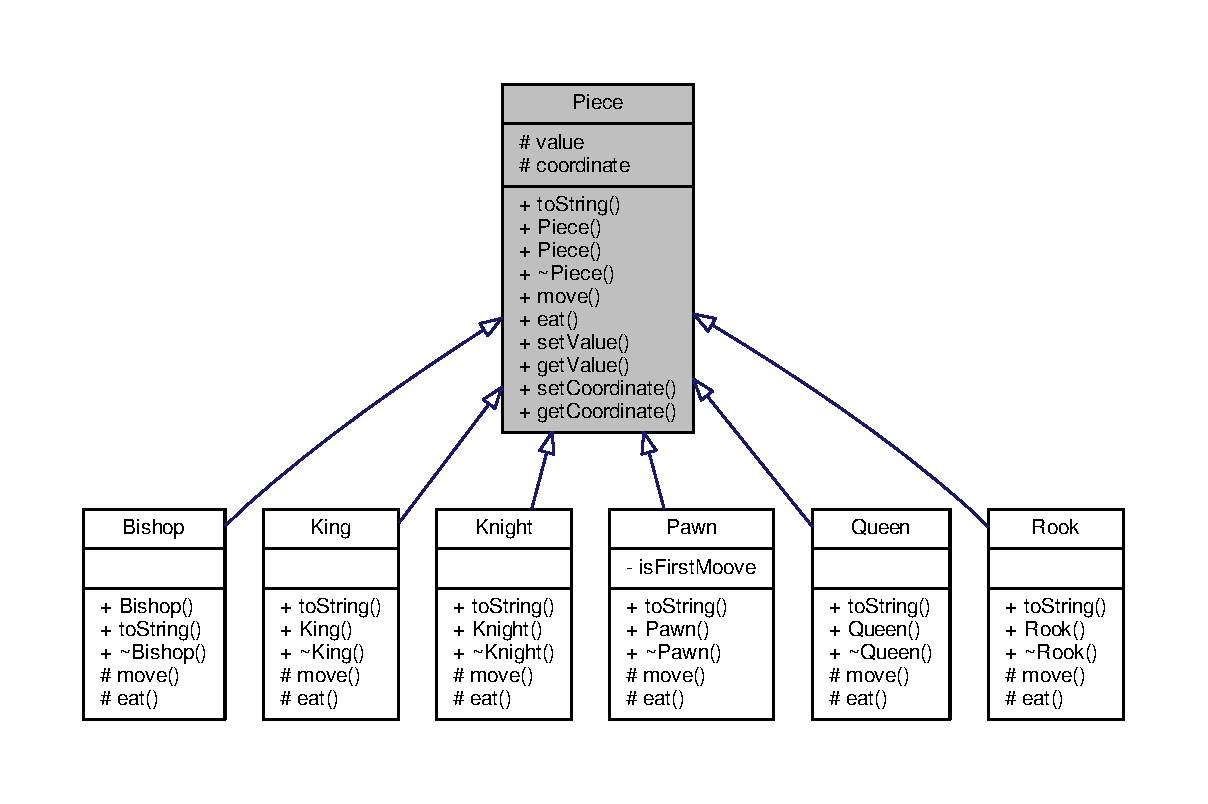
\includegraphics[width=350pt]{class_piece__inherit__graph}
\end{center}
\end{figure}


Collaboration diagram for Piece\+:\nopagebreak
\begin{figure}[H]
\begin{center}
\leavevmode
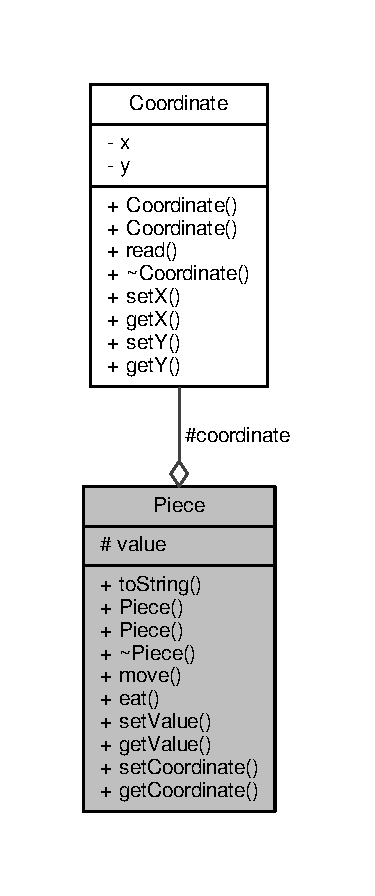
\includegraphics[width=180pt]{class_piece__coll__graph}
\end{center}
\end{figure}
\subsection*{Public Member Functions}
\begin{DoxyCompactItemize}
\item 
virtual std\+::string \hyperlink{class_piece_a2a017f933a49e17d9a60a665ee9df605}{to\+String} ()=0
\item 
\hyperlink{class_piece_afc89acd5b05abd2f8fa4f60ee7ca3b20}{Piece} (unsigned int var\+\_\+temp)
\item 
\hyperlink{class_piece_af1ce807c73a4b82abf28161ea07a95a2}{Piece} (unsigned int var\+\_\+temp, \hyperlink{class_coordinate}{Coordinate} \hyperlink{class_piece_a9e92373c8fffc1f5efb20d62204b70cf}{coordinate})
\item 
virtual \hyperlink{class_piece_a5d7a4f6bade94cb33b6f634de8aa7918}{$\sim$\+Piece} ()
\item 
virtual bool \hyperlink{class_piece_a4939b8f41018950374d294b256906ec3}{move} (\hyperlink{class_coordinate}{Coordinate} t\+\_\+coordinate, \hyperlink{class_board}{Board} $\ast$board)=0
\item 
virtual bool \hyperlink{class_piece_a94fffb0c34e637910c08ded95185e135}{eat} (\hyperlink{class_coordinate}{Coordinate} t\+\_\+coordinate, \hyperlink{class_board}{Board} $\ast$board)=0
\item 
void \hyperlink{class_piece_a889ea7d9eb4b691a07143e9084382b2a}{set\+Value} (unsigned int new\+\_\+var)
\item 
unsigned int \hyperlink{class_piece_a83cba58885b2a385c6b858c1df33de29}{get\+Value} ()
\item 
void \hyperlink{class_piece_aadf96b2e3cdf28dcc52f670f8bc4e0f5}{set\+Coordinate} (\hyperlink{class_coordinate}{Coordinate} new\+\_\+var)
\item 
\hyperlink{class_coordinate}{Coordinate} \hyperlink{class_piece_a847e09b148d9b7125ef9ef8f1d970862}{get\+Coordinate} ()
\end{DoxyCompactItemize}
\subsection*{Protected Attributes}
\begin{DoxyCompactItemize}
\item 
unsigned int \hyperlink{class_piece_a8933ca826f6c9b958f781eaa0160c2b7}{value}
\item 
\hyperlink{class_coordinate}{Coordinate} \hyperlink{class_piece_a9e92373c8fffc1f5efb20d62204b70cf}{coordinate}
\end{DoxyCompactItemize}


\subsection{Constructor \& Destructor Documentation}
\index{Piece@{Piece}!Piece@{Piece}}
\index{Piece@{Piece}!Piece@{Piece}}
\subsubsection[{\texorpdfstring{Piece(unsigned int var\+\_\+temp)}{Piece(unsigned int var_temp)}}]{\setlength{\rightskip}{0pt plus 5cm}Piece\+::\+Piece (
\begin{DoxyParamCaption}
\item[{unsigned int}]{var\+\_\+temp}
\end{DoxyParamCaption}
)}\hypertarget{class_piece_afc89acd5b05abd2f8fa4f60ee7ca3b20}{}\label{class_piece_afc89acd5b05abd2f8fa4f60ee7ca3b20}
Empty Constructor \index{Piece@{Piece}!Piece@{Piece}}
\index{Piece@{Piece}!Piece@{Piece}}
\subsubsection[{\texorpdfstring{Piece(unsigned int var\+\_\+temp, Coordinate coordinate)}{Piece(unsigned int var_temp, Coordinate coordinate)}}]{\setlength{\rightskip}{0pt plus 5cm}Piece\+::\+Piece (
\begin{DoxyParamCaption}
\item[{unsigned int}]{var\+\_\+temp, }
\item[{{\bf Coordinate}}]{coordinate}
\end{DoxyParamCaption}
)}\hypertarget{class_piece_af1ce807c73a4b82abf28161ea07a95a2}{}\label{class_piece_af1ce807c73a4b82abf28161ea07a95a2}
\index{Piece@{Piece}!````~Piece@{$\sim$\+Piece}}
\index{````~Piece@{$\sim$\+Piece}!Piece@{Piece}}
\subsubsection[{\texorpdfstring{$\sim$\+Piece()}{~Piece()}}]{\setlength{\rightskip}{0pt plus 5cm}Piece\+::$\sim$\+Piece (
\begin{DoxyParamCaption}
{}
\end{DoxyParamCaption}
)\hspace{0.3cm}{\ttfamily [virtual]}}\hypertarget{class_piece_a5d7a4f6bade94cb33b6f634de8aa7918}{}\label{class_piece_a5d7a4f6bade94cb33b6f634de8aa7918}
Empty Destructor 

\subsection{Member Function Documentation}
\index{Piece@{Piece}!eat@{eat}}
\index{eat@{eat}!Piece@{Piece}}
\subsubsection[{\texorpdfstring{eat(\+Coordinate t\+\_\+coordinate, Board $\ast$board)=0}{eat(Coordinate t_coordinate, Board *board)=0}}]{\setlength{\rightskip}{0pt plus 5cm}virtual bool Piece\+::eat (
\begin{DoxyParamCaption}
\item[{{\bf Coordinate}}]{t\+\_\+coordinate, }
\item[{{\bf Board} $\ast$}]{board}
\end{DoxyParamCaption}
)\hspace{0.3cm}{\ttfamily [pure virtual]}}\hypertarget{class_piece_a94fffb0c34e637910c08ded95185e135}{}\label{class_piece_a94fffb0c34e637910c08ded95185e135}


Implemented in \hyperlink{class_bishop_a2ff965d9d180e94989953544f0e9ae9b}{Bishop}, \hyperlink{class_king_abd8a9ef79a3a139afa83c2814edc852e}{King}, \hyperlink{class_knight_a5f92f60471d409e3afddefd760d993ec}{Knight}, \hyperlink{class_queen_adc0da381a4d81ba55cbdbd574e1ba7c9}{Queen}, \hyperlink{class_pawn_a3a6fd81c625f8df7d2ae90520c0937fe}{Pawn}, and \hyperlink{class_rook_aeb942bed9da83e30ab23d214e60597a6}{Rook}.

\index{Piece@{Piece}!get\+Coordinate@{get\+Coordinate}}
\index{get\+Coordinate@{get\+Coordinate}!Piece@{Piece}}
\subsubsection[{\texorpdfstring{get\+Coordinate()}{getCoordinate()}}]{\setlength{\rightskip}{0pt plus 5cm}{\bf Coordinate} Piece\+::get\+Coordinate (
\begin{DoxyParamCaption}
{}
\end{DoxyParamCaption}
)\hspace{0.3cm}{\ttfamily [inline]}}\hypertarget{class_piece_a847e09b148d9b7125ef9ef8f1d970862}{}\label{class_piece_a847e09b148d9b7125ef9ef8f1d970862}
Get the value of coordinate \begin{DoxyReturn}{Returns}
the value of coordinate 
\end{DoxyReturn}
\index{Piece@{Piece}!get\+Value@{get\+Value}}
\index{get\+Value@{get\+Value}!Piece@{Piece}}
\subsubsection[{\texorpdfstring{get\+Value()}{getValue()}}]{\setlength{\rightskip}{0pt plus 5cm}unsigned int Piece\+::get\+Value (
\begin{DoxyParamCaption}
{}
\end{DoxyParamCaption}
)\hspace{0.3cm}{\ttfamily [inline]}}\hypertarget{class_piece_a83cba58885b2a385c6b858c1df33de29}{}\label{class_piece_a83cba58885b2a385c6b858c1df33de29}
Get the value of value \begin{DoxyReturn}{Returns}
the value of value 
\end{DoxyReturn}
\index{Piece@{Piece}!move@{move}}
\index{move@{move}!Piece@{Piece}}
\subsubsection[{\texorpdfstring{move(\+Coordinate t\+\_\+coordinate, Board $\ast$board)=0}{move(Coordinate t_coordinate, Board *board)=0}}]{\setlength{\rightskip}{0pt plus 5cm}virtual bool Piece\+::move (
\begin{DoxyParamCaption}
\item[{{\bf Coordinate}}]{t\+\_\+coordinate, }
\item[{{\bf Board} $\ast$}]{board}
\end{DoxyParamCaption}
)\hspace{0.3cm}{\ttfamily [pure virtual]}}\hypertarget{class_piece_a4939b8f41018950374d294b256906ec3}{}\label{class_piece_a4939b8f41018950374d294b256906ec3}


Implemented in \hyperlink{class_bishop_afddd21905462db28e4f3f694d3f156df}{Bishop}, \hyperlink{class_king_ac9319f67056661e2cf0abe05a78407ee}{King}, \hyperlink{class_knight_a852359fbd2d2d5e00445d07c3ec6fdfe}{Knight}, \hyperlink{class_queen_afe77ad943cc3300d822d8b9d18598737}{Queen}, \hyperlink{class_pawn_ae5ac3a2e71798fc8b6226bb9590497ea}{Pawn}, and \hyperlink{class_rook_ad6102df705a5dccea646d8afcbd72ae4}{Rook}.

\index{Piece@{Piece}!set\+Coordinate@{set\+Coordinate}}
\index{set\+Coordinate@{set\+Coordinate}!Piece@{Piece}}
\subsubsection[{\texorpdfstring{set\+Coordinate(\+Coordinate new\+\_\+var)}{setCoordinate(Coordinate new_var)}}]{\setlength{\rightskip}{0pt plus 5cm}void Piece\+::set\+Coordinate (
\begin{DoxyParamCaption}
\item[{{\bf Coordinate}}]{new\+\_\+var}
\end{DoxyParamCaption}
)\hspace{0.3cm}{\ttfamily [inline]}}\hypertarget{class_piece_aadf96b2e3cdf28dcc52f670f8bc4e0f5}{}\label{class_piece_aadf96b2e3cdf28dcc52f670f8bc4e0f5}
\begin{DoxyReturn}{Returns}
bool 
\end{DoxyReturn}

\begin{DoxyParams}{Parameters}
{\em board} & \\
\hline
{\em coordinate} & Set the value of coordinate \\
\hline
{\em new\+\_\+var} & the new value of coordinate \\
\hline
\end{DoxyParams}
\index{Piece@{Piece}!set\+Value@{set\+Value}}
\index{set\+Value@{set\+Value}!Piece@{Piece}}
\subsubsection[{\texorpdfstring{set\+Value(unsigned int new\+\_\+var)}{setValue(unsigned int new_var)}}]{\setlength{\rightskip}{0pt plus 5cm}void Piece\+::set\+Value (
\begin{DoxyParamCaption}
\item[{unsigned int}]{new\+\_\+var}
\end{DoxyParamCaption}
)\hspace{0.3cm}{\ttfamily [inline]}}\hypertarget{class_piece_a889ea7d9eb4b691a07143e9084382b2a}{}\label{class_piece_a889ea7d9eb4b691a07143e9084382b2a}
Set the value of value 
\begin{DoxyParams}{Parameters}
{\em new\+\_\+var} & the new value of value \\
\hline
\end{DoxyParams}
\index{Piece@{Piece}!to\+String@{to\+String}}
\index{to\+String@{to\+String}!Piece@{Piece}}
\subsubsection[{\texorpdfstring{to\+String()=0}{toString()=0}}]{\setlength{\rightskip}{0pt plus 5cm}virtual std\+::string Piece\+::to\+String (
\begin{DoxyParamCaption}
{}
\end{DoxyParamCaption}
)\hspace{0.3cm}{\ttfamily [pure virtual]}}\hypertarget{class_piece_a2a017f933a49e17d9a60a665ee9df605}{}\label{class_piece_a2a017f933a49e17d9a60a665ee9df605}


Implemented in \hyperlink{class_bishop_af69ba4eec8bcf5dad66c8071a168bdba}{Bishop}, \hyperlink{class_king_a445fa11a84a95f5257eea4fb0a4f4839}{King}, \hyperlink{class_pawn_afac4abaf92106777e20d21fde635ffc4}{Pawn}, \hyperlink{class_queen_a1cf5f21870e6b2ec107a9e3280a69da6}{Queen}, \hyperlink{class_rook_a6b9d17ae219d74742a7deacf52aa4641}{Rook}, and \hyperlink{class_knight_a3ecdeb255fa07eaa22d0cc948520c181}{Knight}.



\subsection{Member Data Documentation}
\index{Piece@{Piece}!coordinate@{coordinate}}
\index{coordinate@{coordinate}!Piece@{Piece}}
\subsubsection[{\texorpdfstring{coordinate}{coordinate}}]{\setlength{\rightskip}{0pt plus 5cm}{\bf Coordinate} Piece\+::coordinate\hspace{0.3cm}{\ttfamily [protected]}}\hypertarget{class_piece_a9e92373c8fffc1f5efb20d62204b70cf}{}\label{class_piece_a9e92373c8fffc1f5efb20d62204b70cf}
\index{Piece@{Piece}!value@{value}}
\index{value@{value}!Piece@{Piece}}
\subsubsection[{\texorpdfstring{value}{value}}]{\setlength{\rightskip}{0pt plus 5cm}unsigned int Piece\+::value\hspace{0.3cm}{\ttfamily [protected]}}\hypertarget{class_piece_a8933ca826f6c9b958f781eaa0160c2b7}{}\label{class_piece_a8933ca826f6c9b958f781eaa0160c2b7}


The documentation for this class was generated from the following files\+:\begin{DoxyCompactItemize}
\item 
\hyperlink{_piece_8h}{Piece.\+h}\item 
\hyperlink{_piece_8cpp}{Piece.\+cpp}\end{DoxyCompactItemize}

\hypertarget{class_player}{}\section{Player Class Reference}
\label{class_player}\index{Player@{Player}}


{\ttfamily \#include $<$Player.\+h$>$}



Collaboration diagram for Player\+:
\nopagebreak
\begin{figure}[H]
\begin{center}
\leavevmode
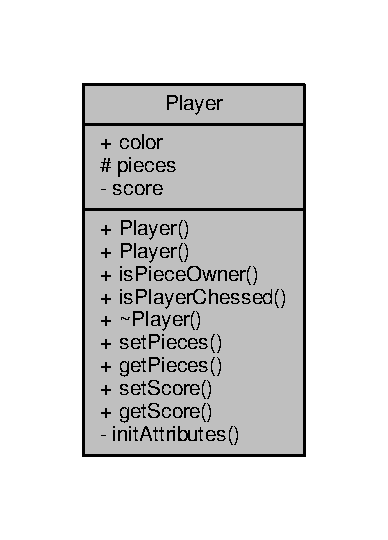
\includegraphics[width=186pt]{class_player__coll__graph}
\end{center}
\end{figure}
\subsection*{Public Member Functions}
\begin{DoxyCompactItemize}
\item 
\hyperlink{class_player_affe0cc3cb714f6deb4e62f0c0d3f1fd8}{Player} ()
\item 
\hyperlink{class_player_a355464bd2331faa49dfcc259174ac0ee}{Player} (std\+::string color\+\_\+temp)
\item 
bool \hyperlink{class_player_acd154fbc75679e8bd21ae790836c8623}{is\+Piece\+Owner} (\hyperlink{class_piece}{Piece} $\ast$piece)
\item 
bool \hyperlink{class_player_ab792f06e8da9ce878b2de013fb04b103}{is\+Player\+Chessed} (\hyperlink{class_board}{Board} $\ast$board)
\item 
virtual \hyperlink{class_player_a749d2c00e1fe0f5c2746f7505a58c062}{$\sim$\+Player} ()
\item 
void \hyperlink{class_player_a31d381a29c010c26d69a4cfd30c37049}{set\+Pieces} (std\+::list$<$ \hyperlink{class_piece}{Piece} $\ast$ $>$ new\+\_\+var)
\item 
std\+::list$<$ \hyperlink{class_piece}{Piece} $\ast$ $>$ \& \hyperlink{class_player_a479c15c00634b36e3391443afe5b9b80}{get\+Pieces} ()
\item 
void \hyperlink{class_player_ae02f0030bc93cd08c014dd48943c0304}{set\+Score} (unsigned int new\+\_\+var)
\item 
unsigned int \hyperlink{class_player_a0a4b4a42bca1b1d62be928ce234d8df5}{get\+Score} ()
\end{DoxyCompactItemize}
\subsection*{Public Attributes}
\begin{DoxyCompactItemize}
\item 
std\+::string \hyperlink{class_player_ac2e6856437961bb592e38ecb40c2f348}{color}
\end{DoxyCompactItemize}
\subsection*{Protected Attributes}
\begin{DoxyCompactItemize}
\item 
std\+::list$<$ \hyperlink{class_piece}{Piece} $\ast$ $>$ \hyperlink{class_player_aae72d6ce61d41bee8d04318baa36b239}{pieces}
\end{DoxyCompactItemize}
\subsection*{Private Member Functions}
\begin{DoxyCompactItemize}
\item 
void \hyperlink{class_player_acd7645a07397ed3d4a499b139784eeb3}{init\+Attributes} ()
\end{DoxyCompactItemize}
\subsection*{Private Attributes}
\begin{DoxyCompactItemize}
\item 
unsigned int \hyperlink{class_player_a38a6dafe988a768a435cc0a9fde38e46}{score}
\end{DoxyCompactItemize}


\subsection{Detailed Description}
class \hyperlink{class_player}{Player} 

\subsection{Constructor \& Destructor Documentation}
\index{Player@{Player}!Player@{Player}}
\index{Player@{Player}!Player@{Player}}
\subsubsection[{\texorpdfstring{Player()}{Player()}}]{\setlength{\rightskip}{0pt plus 5cm}Player\+::\+Player (
\begin{DoxyParamCaption}
{}
\end{DoxyParamCaption}
)}\hypertarget{class_player_affe0cc3cb714f6deb4e62f0c0d3f1fd8}{}\label{class_player_affe0cc3cb714f6deb4e62f0c0d3f1fd8}
Empty Constructor \index{Player@{Player}!Player@{Player}}
\index{Player@{Player}!Player@{Player}}
\subsubsection[{\texorpdfstring{Player(std\+::string color\+\_\+temp)}{Player(std::string color_temp)}}]{\setlength{\rightskip}{0pt plus 5cm}Player\+::\+Player (
\begin{DoxyParamCaption}
\item[{std\+::string}]{color\+\_\+temp}
\end{DoxyParamCaption}
)}\hypertarget{class_player_a355464bd2331faa49dfcc259174ac0ee}{}\label{class_player_a355464bd2331faa49dfcc259174ac0ee}
\index{Player@{Player}!````~Player@{$\sim$\+Player}}
\index{````~Player@{$\sim$\+Player}!Player@{Player}}
\subsubsection[{\texorpdfstring{$\sim$\+Player()}{~Player()}}]{\setlength{\rightskip}{0pt plus 5cm}Player\+::$\sim$\+Player (
\begin{DoxyParamCaption}
{}
\end{DoxyParamCaption}
)\hspace{0.3cm}{\ttfamily [virtual]}}\hypertarget{class_player_a749d2c00e1fe0f5c2746f7505a58c062}{}\label{class_player_a749d2c00e1fe0f5c2746f7505a58c062}
Empty Destructor 

\subsection{Member Function Documentation}
\index{Player@{Player}!get\+Pieces@{get\+Pieces}}
\index{get\+Pieces@{get\+Pieces}!Player@{Player}}
\subsubsection[{\texorpdfstring{get\+Pieces()}{getPieces()}}]{\setlength{\rightskip}{0pt plus 5cm}std\+::list$<${\bf Piece}$\ast$$>$\& Player\+::get\+Pieces (
\begin{DoxyParamCaption}
{}
\end{DoxyParamCaption}
)\hspace{0.3cm}{\ttfamily [inline]}}\hypertarget{class_player_a479c15c00634b36e3391443afe5b9b80}{}\label{class_player_a479c15c00634b36e3391443afe5b9b80}
Get the value of pieces \begin{DoxyReturn}{Returns}
the value of pieces 
\end{DoxyReturn}
\index{Player@{Player}!get\+Score@{get\+Score}}
\index{get\+Score@{get\+Score}!Player@{Player}}
\subsubsection[{\texorpdfstring{get\+Score()}{getScore()}}]{\setlength{\rightskip}{0pt plus 5cm}unsigned int Player\+::get\+Score (
\begin{DoxyParamCaption}
{}
\end{DoxyParamCaption}
)\hspace{0.3cm}{\ttfamily [inline]}}\hypertarget{class_player_a0a4b4a42bca1b1d62be928ce234d8df5}{}\label{class_player_a0a4b4a42bca1b1d62be928ce234d8df5}
Get the value of score \begin{DoxyReturn}{Returns}
the value of score 
\end{DoxyReturn}
\index{Player@{Player}!init\+Attributes@{init\+Attributes}}
\index{init\+Attributes@{init\+Attributes}!Player@{Player}}
\subsubsection[{\texorpdfstring{init\+Attributes()}{initAttributes()}}]{\setlength{\rightskip}{0pt plus 5cm}void Player\+::init\+Attributes (
\begin{DoxyParamCaption}
{}
\end{DoxyParamCaption}
)\hspace{0.3cm}{\ttfamily [private]}}\hypertarget{class_player_acd7645a07397ed3d4a499b139784eeb3}{}\label{class_player_acd7645a07397ed3d4a499b139784eeb3}
\index{Player@{Player}!is\+Piece\+Owner@{is\+Piece\+Owner}}
\index{is\+Piece\+Owner@{is\+Piece\+Owner}!Player@{Player}}
\subsubsection[{\texorpdfstring{is\+Piece\+Owner(\+Piece $\ast$piece)}{isPieceOwner(Piece *piece)}}]{\setlength{\rightskip}{0pt plus 5cm}bool Player\+::is\+Piece\+Owner (
\begin{DoxyParamCaption}
\item[{{\bf Piece} $\ast$}]{piece}
\end{DoxyParamCaption}
)}\hypertarget{class_player_acd154fbc75679e8bd21ae790836c8623}{}\label{class_player_acd154fbc75679e8bd21ae790836c8623}
\index{Player@{Player}!is\+Player\+Chessed@{is\+Player\+Chessed}}
\index{is\+Player\+Chessed@{is\+Player\+Chessed}!Player@{Player}}
\subsubsection[{\texorpdfstring{is\+Player\+Chessed(\+Board $\ast$board)}{isPlayerChessed(Board *board)}}]{\setlength{\rightskip}{0pt plus 5cm}bool Player\+::is\+Player\+Chessed (
\begin{DoxyParamCaption}
\item[{{\bf Board} $\ast$}]{board}
\end{DoxyParamCaption}
)}\hypertarget{class_player_ab792f06e8da9ce878b2de013fb04b103}{}\label{class_player_ab792f06e8da9ce878b2de013fb04b103}






\index{Player@{Player}!set\+Pieces@{set\+Pieces}}
\index{set\+Pieces@{set\+Pieces}!Player@{Player}}
\subsubsection[{\texorpdfstring{set\+Pieces(std\+::list$<$ Piece $\ast$ $>$ new\+\_\+var)}{setPieces(std::list< Piece * > new_var)}}]{\setlength{\rightskip}{0pt plus 5cm}void Player\+::set\+Pieces (
\begin{DoxyParamCaption}
\item[{std\+::list$<$ {\bf Piece} $\ast$ $>$}]{new\+\_\+var}
\end{DoxyParamCaption}
)\hspace{0.3cm}{\ttfamily [inline]}}\hypertarget{class_player_a31d381a29c010c26d69a4cfd30c37049}{}\label{class_player_a31d381a29c010c26d69a4cfd30c37049}
Set the value of pieces 
\begin{DoxyParams}{Parameters}
{\em new\+\_\+var} & the new value of pieces \\
\hline
\end{DoxyParams}
\index{Player@{Player}!set\+Score@{set\+Score}}
\index{set\+Score@{set\+Score}!Player@{Player}}
\subsubsection[{\texorpdfstring{set\+Score(unsigned int new\+\_\+var)}{setScore(unsigned int new_var)}}]{\setlength{\rightskip}{0pt plus 5cm}void Player\+::set\+Score (
\begin{DoxyParamCaption}
\item[{unsigned int}]{new\+\_\+var}
\end{DoxyParamCaption}
)\hspace{0.3cm}{\ttfamily [inline]}}\hypertarget{class_player_ae02f0030bc93cd08c014dd48943c0304}{}\label{class_player_ae02f0030bc93cd08c014dd48943c0304}
Set the value of score 
\begin{DoxyParams}{Parameters}
{\em new\+\_\+var} & the new value of score \\
\hline
\end{DoxyParams}


\subsection{Member Data Documentation}
\index{Player@{Player}!color@{color}}
\index{color@{color}!Player@{Player}}
\subsubsection[{\texorpdfstring{color}{color}}]{\setlength{\rightskip}{0pt plus 5cm}std\+::string Player\+::color}\hypertarget{class_player_ac2e6856437961bb592e38ecb40c2f348}{}\label{class_player_ac2e6856437961bb592e38ecb40c2f348}
\index{Player@{Player}!pieces@{pieces}}
\index{pieces@{pieces}!Player@{Player}}
\subsubsection[{\texorpdfstring{pieces}{pieces}}]{\setlength{\rightskip}{0pt plus 5cm}std\+::list$<${\bf Piece}$\ast$$>$ Player\+::pieces\hspace{0.3cm}{\ttfamily [protected]}}\hypertarget{class_player_aae72d6ce61d41bee8d04318baa36b239}{}\label{class_player_aae72d6ce61d41bee8d04318baa36b239}
\index{Player@{Player}!score@{score}}
\index{score@{score}!Player@{Player}}
\subsubsection[{\texorpdfstring{score}{score}}]{\setlength{\rightskip}{0pt plus 5cm}unsigned int Player\+::score\hspace{0.3cm}{\ttfamily [private]}}\hypertarget{class_player_a38a6dafe988a768a435cc0a9fde38e46}{}\label{class_player_a38a6dafe988a768a435cc0a9fde38e46}


The documentation for this class was generated from the following files\+:\begin{DoxyCompactItemize}
\item 
\hyperlink{_player_8h}{Player.\+h}\item 
\hyperlink{_player_8cpp}{Player.\+cpp}\end{DoxyCompactItemize}

\hypertarget{class_queen}{}\section{Queen Class Reference}
\label{class_queen}\index{Queen@{Queen}}


{\ttfamily \#include $<$Queen.\+h$>$}



Inheritance diagram for Queen\+:
\nopagebreak
\begin{figure}[H]
\begin{center}
\leavevmode
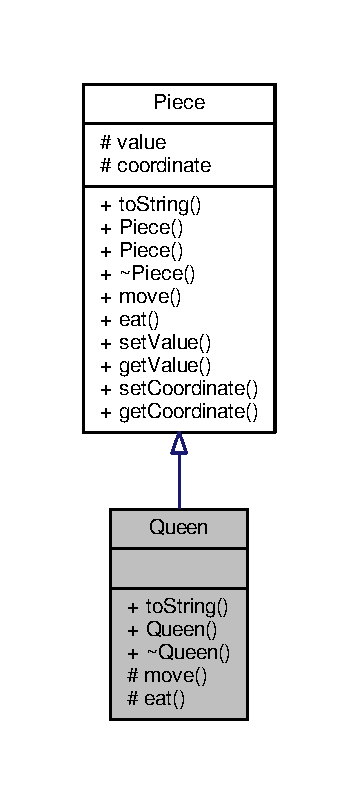
\includegraphics[width=172pt]{class_queen__inherit__graph}
\end{center}
\end{figure}


Collaboration diagram for Queen\+:
\nopagebreak
\begin{figure}[H]
\begin{center}
\leavevmode
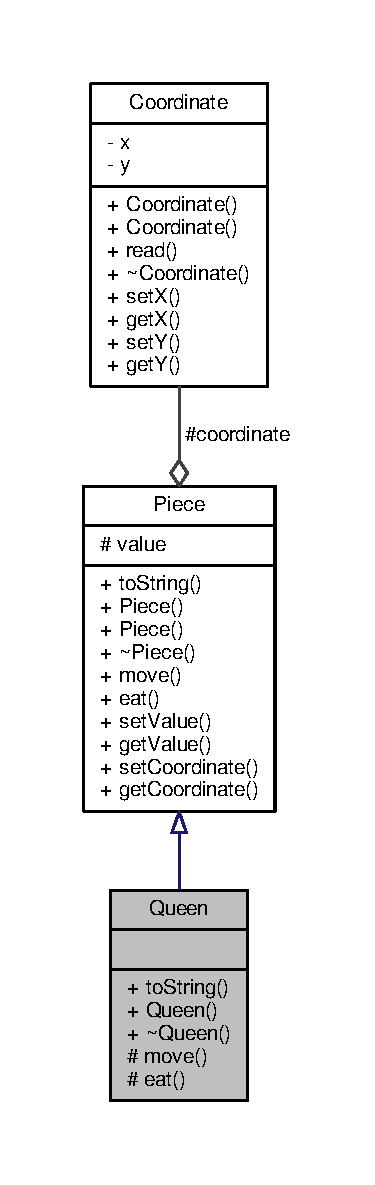
\includegraphics[height=550pt]{class_queen__coll__graph}
\end{center}
\end{figure}
\subsection*{Public Member Functions}
\begin{DoxyCompactItemize}
\item 
virtual std\+::string \hyperlink{class_queen_a1cf5f21870e6b2ec107a9e3280a69da6}{to\+String} ()
\item 
\hyperlink{class_queen_ab0d98820ff74906af19e0b7495348f8b}{Queen} (\hyperlink{class_coordinate}{Coordinate} \hyperlink{class_piece_a9e92373c8fffc1f5efb20d62204b70cf}{coordinate})
\item 
virtual \hyperlink{class_queen_aa22f6c1a49a583b549bd1f940e50721d}{$\sim$\+Queen} ()
\end{DoxyCompactItemize}
\subsection*{Protected Member Functions}
\begin{DoxyCompactItemize}
\item 
virtual bool \hyperlink{class_queen_afe77ad943cc3300d822d8b9d18598737}{move} (\hyperlink{class_coordinate}{Coordinate} \hyperlink{class_piece_a9e92373c8fffc1f5efb20d62204b70cf}{coordinate}, \hyperlink{class_board}{Board} $\ast$board)
\item 
virtual bool \hyperlink{class_queen_adc0da381a4d81ba55cbdbd574e1ba7c9}{eat} (\hyperlink{class_coordinate}{Coordinate} \hyperlink{class_piece_a9e92373c8fffc1f5efb20d62204b70cf}{coordinate}, \hyperlink{class_board}{Board} $\ast$board)
\end{DoxyCompactItemize}
\subsection*{Additional Inherited Members}


\subsection{Detailed Description}
class \hyperlink{class_queen}{Queen} 

\subsection{Constructor \& Destructor Documentation}
\index{Queen@{Queen}!Queen@{Queen}}
\index{Queen@{Queen}!Queen@{Queen}}
\subsubsection[{\texorpdfstring{Queen(\+Coordinate coordinate)}{Queen(Coordinate coordinate)}}]{\setlength{\rightskip}{0pt plus 5cm}Queen\+::\+Queen (
\begin{DoxyParamCaption}
\item[{{\bf Coordinate}}]{coordinate}
\end{DoxyParamCaption}
)}\hypertarget{class_queen_ab0d98820ff74906af19e0b7495348f8b}{}\label{class_queen_ab0d98820ff74906af19e0b7495348f8b}
Empty Constructor \index{Queen@{Queen}!````~Queen@{$\sim$\+Queen}}
\index{````~Queen@{$\sim$\+Queen}!Queen@{Queen}}
\subsubsection[{\texorpdfstring{$\sim$\+Queen()}{~Queen()}}]{\setlength{\rightskip}{0pt plus 5cm}Queen\+::$\sim$\+Queen (
\begin{DoxyParamCaption}
{}
\end{DoxyParamCaption}
)\hspace{0.3cm}{\ttfamily [virtual]}}\hypertarget{class_queen_aa22f6c1a49a583b549bd1f940e50721d}{}\label{class_queen_aa22f6c1a49a583b549bd1f940e50721d}
Empty Destructor 

\subsection{Member Function Documentation}
\index{Queen@{Queen}!eat@{eat}}
\index{eat@{eat}!Queen@{Queen}}
\subsubsection[{\texorpdfstring{eat(\+Coordinate coordinate, Board $\ast$board)}{eat(Coordinate coordinate, Board *board)}}]{\setlength{\rightskip}{0pt plus 5cm}bool Queen\+::eat (
\begin{DoxyParamCaption}
\item[{{\bf Coordinate}}]{coordinate, }
\item[{{\bf Board} $\ast$}]{board}
\end{DoxyParamCaption}
)\hspace{0.3cm}{\ttfamily [protected]}, {\ttfamily [virtual]}}\hypertarget{class_queen_adc0da381a4d81ba55cbdbd574e1ba7c9}{}\label{class_queen_adc0da381a4d81ba55cbdbd574e1ba7c9}


Implements \hyperlink{class_piece_a94fffb0c34e637910c08ded95185e135}{Piece}.

\index{Queen@{Queen}!move@{move}}
\index{move@{move}!Queen@{Queen}}
\subsubsection[{\texorpdfstring{move(\+Coordinate coordinate, Board $\ast$board)}{move(Coordinate coordinate, Board *board)}}]{\setlength{\rightskip}{0pt plus 5cm}bool Queen\+::move (
\begin{DoxyParamCaption}
\item[{{\bf Coordinate}}]{coordinate, }
\item[{{\bf Board} $\ast$}]{board}
\end{DoxyParamCaption}
)\hspace{0.3cm}{\ttfamily [protected]}, {\ttfamily [virtual]}}\hypertarget{class_queen_afe77ad943cc3300d822d8b9d18598737}{}\label{class_queen_afe77ad943cc3300d822d8b9d18598737}


Implements \hyperlink{class_piece_a4939b8f41018950374d294b256906ec3}{Piece}.

\index{Queen@{Queen}!to\+String@{to\+String}}
\index{to\+String@{to\+String}!Queen@{Queen}}
\subsubsection[{\texorpdfstring{to\+String()}{toString()}}]{\setlength{\rightskip}{0pt plus 5cm}virtual std\+::string Queen\+::to\+String (
\begin{DoxyParamCaption}
{}
\end{DoxyParamCaption}
)\hspace{0.3cm}{\ttfamily [inline]}, {\ttfamily [virtual]}}\hypertarget{class_queen_a1cf5f21870e6b2ec107a9e3280a69da6}{}\label{class_queen_a1cf5f21870e6b2ec107a9e3280a69da6}


Implements \hyperlink{class_piece_a2a017f933a49e17d9a60a665ee9df605}{Piece}.



The documentation for this class was generated from the following files\+:\begin{DoxyCompactItemize}
\item 
\hyperlink{_queen_8h}{Queen.\+h}\item 
\hyperlink{_queen_8cpp}{Queen.\+cpp}\end{DoxyCompactItemize}

\hypertarget{class_rook}{}\section{Rook Class Reference}
\label{class_rook}\index{Rook@{Rook}}


{\ttfamily \#include $<$Rook.\+h$>$}



Inheritance diagram for Rook\+:
\nopagebreak
\begin{figure}[H]
\begin{center}
\leavevmode
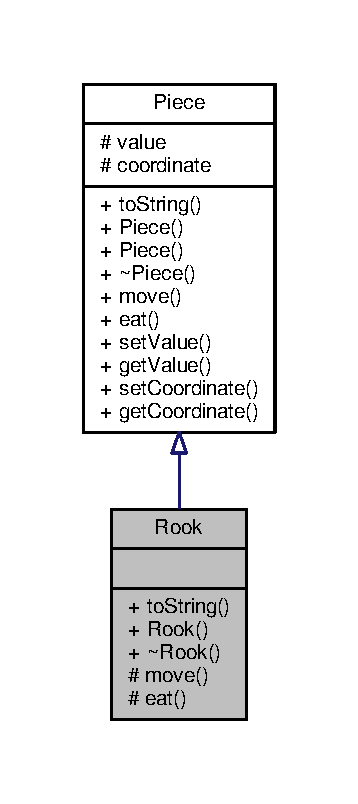
\includegraphics[width=172pt]{class_rook__inherit__graph}
\end{center}
\end{figure}


Collaboration diagram for Rook\+:
\nopagebreak
\begin{figure}[H]
\begin{center}
\leavevmode
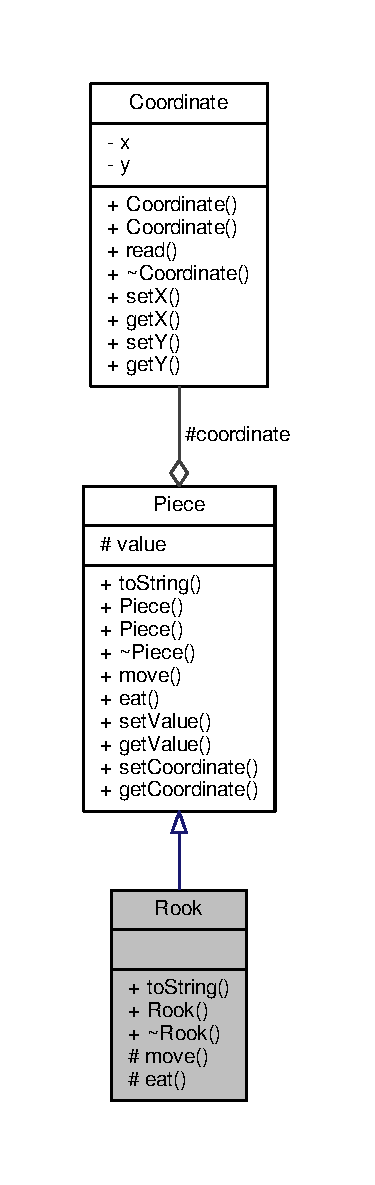
\includegraphics[height=550pt]{class_rook__coll__graph}
\end{center}
\end{figure}
\subsection*{Public Member Functions}
\begin{DoxyCompactItemize}
\item 
virtual std\+::string \hyperlink{class_rook_a6b9d17ae219d74742a7deacf52aa4641}{to\+String} ()
\item 
\hyperlink{class_rook_afbcd69bc8c1a497b7656ddef8ec371f2}{Rook} (\hyperlink{class_coordinate}{Coordinate} \hyperlink{class_piece_a9e92373c8fffc1f5efb20d62204b70cf}{coordinate})
\item 
virtual \hyperlink{class_rook_a70d445b94848b22ded850b6f58bc2972}{$\sim$\+Rook} ()
\end{DoxyCompactItemize}
\subsection*{Protected Member Functions}
\begin{DoxyCompactItemize}
\item 
virtual bool \hyperlink{class_rook_ad6102df705a5dccea646d8afcbd72ae4}{move} (\hyperlink{class_coordinate}{Coordinate} \hyperlink{class_piece_a9e92373c8fffc1f5efb20d62204b70cf}{coordinate}, \hyperlink{class_board}{Board} $\ast$board)
\item 
virtual bool \hyperlink{class_rook_aeb942bed9da83e30ab23d214e60597a6}{eat} (\hyperlink{class_coordinate}{Coordinate} \hyperlink{class_piece_a9e92373c8fffc1f5efb20d62204b70cf}{coordinate}, \hyperlink{class_board}{Board} $\ast$board)
\end{DoxyCompactItemize}
\subsection*{Additional Inherited Members}


\subsection{Detailed Description}
class \hyperlink{class_rook}{Rook} 

\subsection{Constructor \& Destructor Documentation}
\index{Rook@{Rook}!Rook@{Rook}}
\index{Rook@{Rook}!Rook@{Rook}}
\subsubsection[{\texorpdfstring{Rook(\+Coordinate coordinate)}{Rook(Coordinate coordinate)}}]{\setlength{\rightskip}{0pt plus 5cm}Rook\+::\+Rook (
\begin{DoxyParamCaption}
\item[{{\bf Coordinate}}]{coordinate}
\end{DoxyParamCaption}
)}\hypertarget{class_rook_afbcd69bc8c1a497b7656ddef8ec371f2}{}\label{class_rook_afbcd69bc8c1a497b7656ddef8ec371f2}
Empty Constructor \index{Rook@{Rook}!````~Rook@{$\sim$\+Rook}}
\index{````~Rook@{$\sim$\+Rook}!Rook@{Rook}}
\subsubsection[{\texorpdfstring{$\sim$\+Rook()}{~Rook()}}]{\setlength{\rightskip}{0pt plus 5cm}Rook\+::$\sim$\+Rook (
\begin{DoxyParamCaption}
{}
\end{DoxyParamCaption}
)\hspace{0.3cm}{\ttfamily [virtual]}}\hypertarget{class_rook_a70d445b94848b22ded850b6f58bc2972}{}\label{class_rook_a70d445b94848b22ded850b6f58bc2972}
Empty Destructor 

\subsection{Member Function Documentation}
\index{Rook@{Rook}!eat@{eat}}
\index{eat@{eat}!Rook@{Rook}}
\subsubsection[{\texorpdfstring{eat(\+Coordinate coordinate, Board $\ast$board)}{eat(Coordinate coordinate, Board *board)}}]{\setlength{\rightskip}{0pt plus 5cm}bool Rook\+::eat (
\begin{DoxyParamCaption}
\item[{{\bf Coordinate}}]{coordinate, }
\item[{{\bf Board} $\ast$}]{board}
\end{DoxyParamCaption}
)\hspace{0.3cm}{\ttfamily [protected]}, {\ttfamily [virtual]}}\hypertarget{class_rook_aeb942bed9da83e30ab23d214e60597a6}{}\label{class_rook_aeb942bed9da83e30ab23d214e60597a6}


Implements \hyperlink{class_piece_a94fffb0c34e637910c08ded95185e135}{Piece}.

\index{Rook@{Rook}!move@{move}}
\index{move@{move}!Rook@{Rook}}
\subsubsection[{\texorpdfstring{move(\+Coordinate coordinate, Board $\ast$board)}{move(Coordinate coordinate, Board *board)}}]{\setlength{\rightskip}{0pt plus 5cm}bool Rook\+::move (
\begin{DoxyParamCaption}
\item[{{\bf Coordinate}}]{coordinate, }
\item[{{\bf Board} $\ast$}]{board}
\end{DoxyParamCaption}
)\hspace{0.3cm}{\ttfamily [protected]}, {\ttfamily [virtual]}}\hypertarget{class_rook_ad6102df705a5dccea646d8afcbd72ae4}{}\label{class_rook_ad6102df705a5dccea646d8afcbd72ae4}


Implements \hyperlink{class_piece_a4939b8f41018950374d294b256906ec3}{Piece}.

\index{Rook@{Rook}!to\+String@{to\+String}}
\index{to\+String@{to\+String}!Rook@{Rook}}
\subsubsection[{\texorpdfstring{to\+String()}{toString()}}]{\setlength{\rightskip}{0pt plus 5cm}virtual std\+::string Rook\+::to\+String (
\begin{DoxyParamCaption}
{}
\end{DoxyParamCaption}
)\hspace{0.3cm}{\ttfamily [inline]}, {\ttfamily [virtual]}}\hypertarget{class_rook_a6b9d17ae219d74742a7deacf52aa4641}{}\label{class_rook_a6b9d17ae219d74742a7deacf52aa4641}


Implements \hyperlink{class_piece_a2a017f933a49e17d9a60a665ee9df605}{Piece}.



The documentation for this class was generated from the following files\+:\begin{DoxyCompactItemize}
\item 
\hyperlink{_rook_8h}{Rook.\+h}\item 
\hyperlink{_rook_8cpp}{Rook.\+cpp}\end{DoxyCompactItemize}

\chapter{File Documentation}
\hypertarget{_bishop_8cpp}{}\section{Bishop.\+cpp File Reference}
\label{_bishop_8cpp}\index{Bishop.\+cpp@{Bishop.\+cpp}}
{\ttfamily \#include \char`\"{}Bishop.\+h\char`\"{}}\\*
Include dependency graph for Bishop.\+cpp\+:
\nopagebreak
\begin{figure}[H]
\begin{center}
\leavevmode
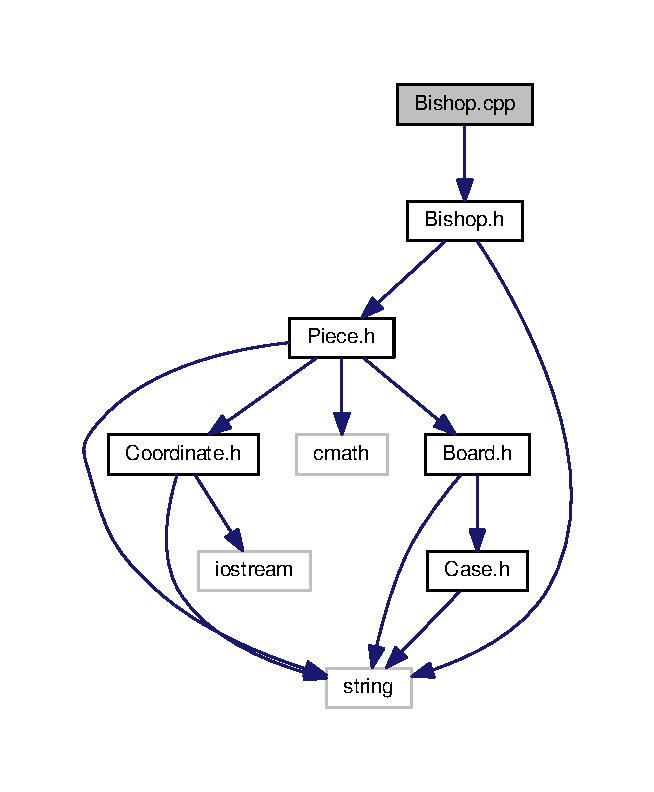
\includegraphics[width=314pt]{_bishop_8cpp__incl}
\end{center}
\end{figure}

\hypertarget{_bishop_8h}{}\section{Bishop.\+h File Reference}
\label{_bishop_8h}\index{Bishop.\+h@{Bishop.\+h}}
{\ttfamily \#include \char`\"{}Piece.\+h\char`\"{}}\\*
{\ttfamily \#include $<$string$>$}\\*
Include dependency graph for Bishop.\+h\+:\nopagebreak
\begin{figure}[H]
\begin{center}
\leavevmode
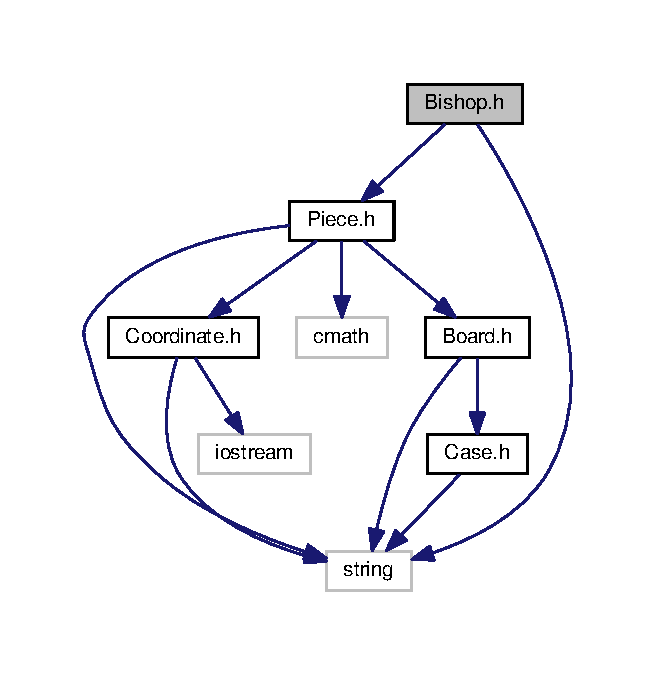
\includegraphics[width=314pt]{_bishop_8h__incl}
\end{center}
\end{figure}
This graph shows which files directly or indirectly include this file\+:\nopagebreak
\begin{figure}[H]
\begin{center}
\leavevmode
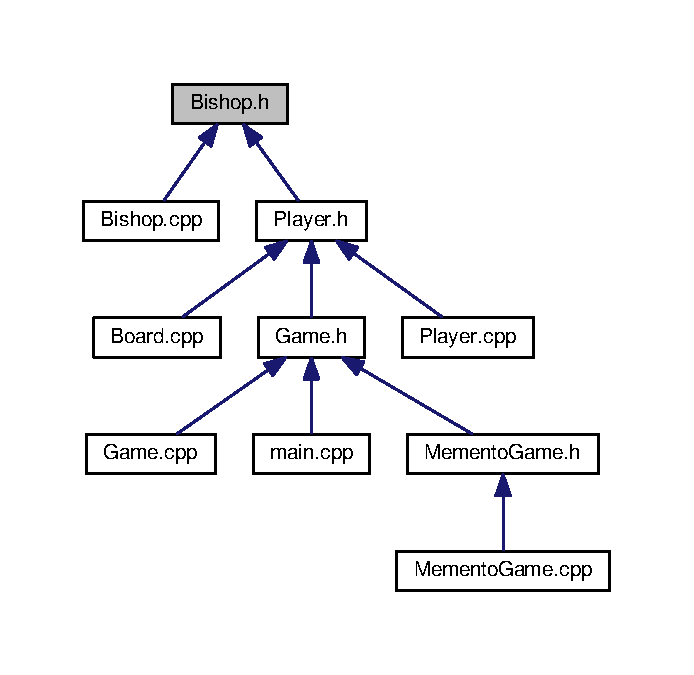
\includegraphics[width=296pt]{_bishop_8h__dep__incl}
\end{center}
\end{figure}
\subsection*{Classes}
\begin{DoxyCompactItemize}
\item 
class \hyperlink{class_bishop}{Bishop}
\end{DoxyCompactItemize}

\hypertarget{_board_8cpp}{}\section{Board.\+cpp File Reference}
\label{_board_8cpp}\index{Board.\+cpp@{Board.\+cpp}}
{\ttfamily \#include \char`\"{}Board.\+h\char`\"{}}\\*
{\ttfamily \#include $<$iostream$>$}\\*
{\ttfamily \#include \char`\"{}Player.\+h\char`\"{}}\\*
Include dependency graph for Board.\+cpp\+:
\nopagebreak
\begin{figure}[H]
\begin{center}
\leavevmode
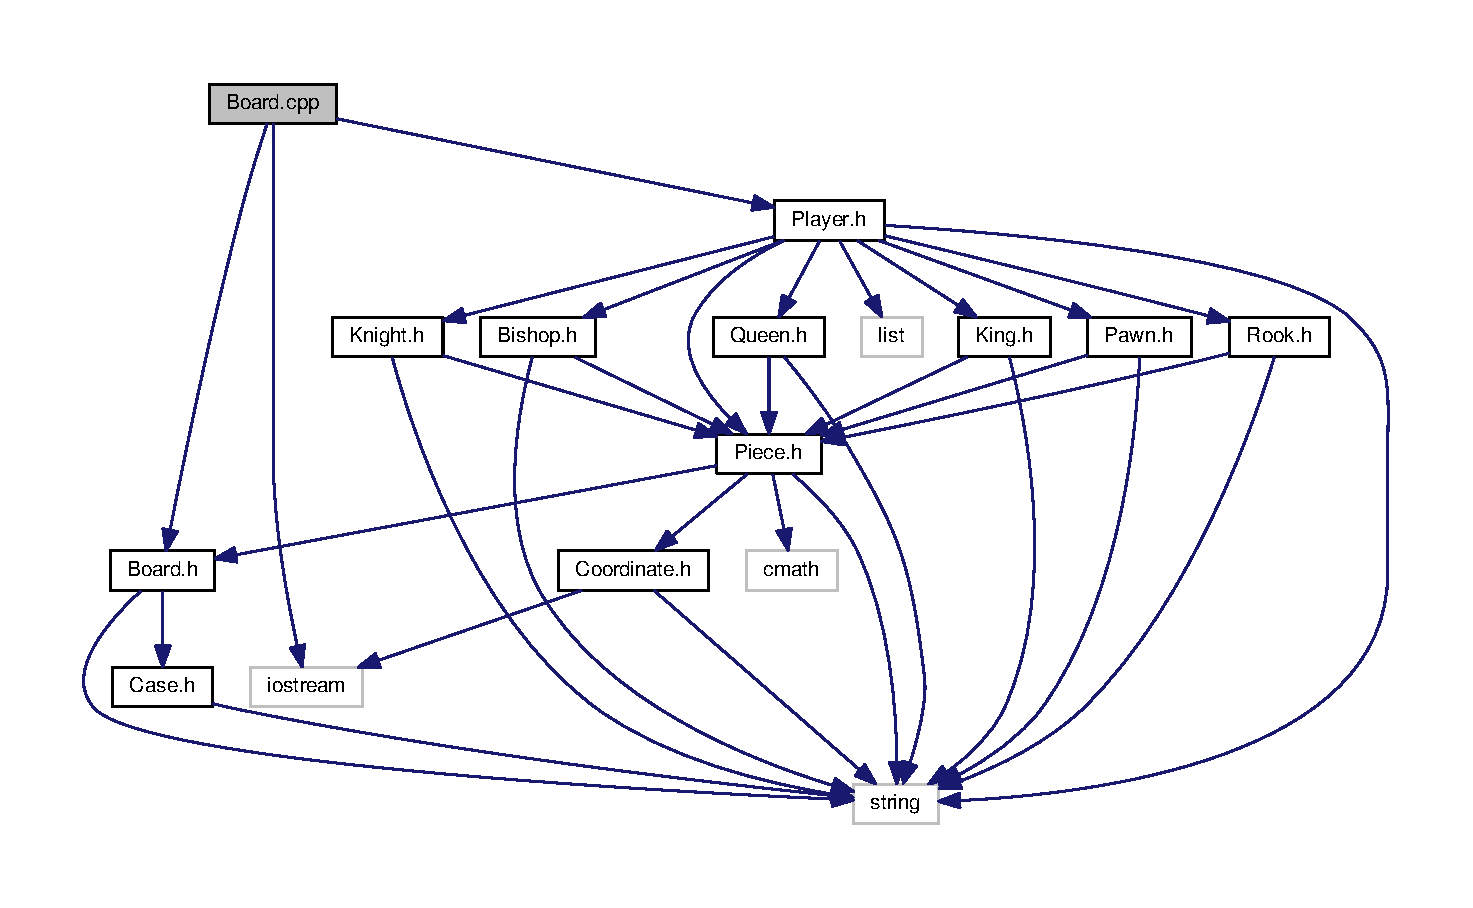
\includegraphics[width=350pt]{_board_8cpp__incl}
\end{center}
\end{figure}

\hypertarget{_board_8h}{}\section{Board.\+h File Reference}
\label{_board_8h}\index{Board.\+h@{Board.\+h}}
{\ttfamily \#include $<$string$>$}\\*
{\ttfamily \#include \char`\"{}Case.\+h\char`\"{}}\\*
Include dependency graph for Board.\+h\+:\nopagebreak
\begin{figure}[H]
\begin{center}
\leavevmode
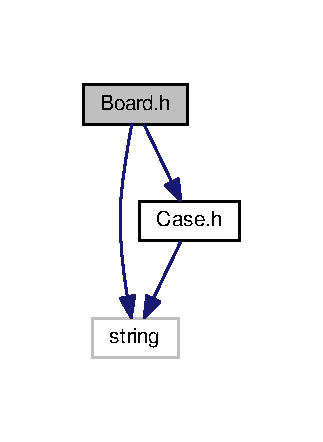
\includegraphics[width=155pt]{_board_8h__incl}
\end{center}
\end{figure}
This graph shows which files directly or indirectly include this file\+:\nopagebreak
\begin{figure}[H]
\begin{center}
\leavevmode
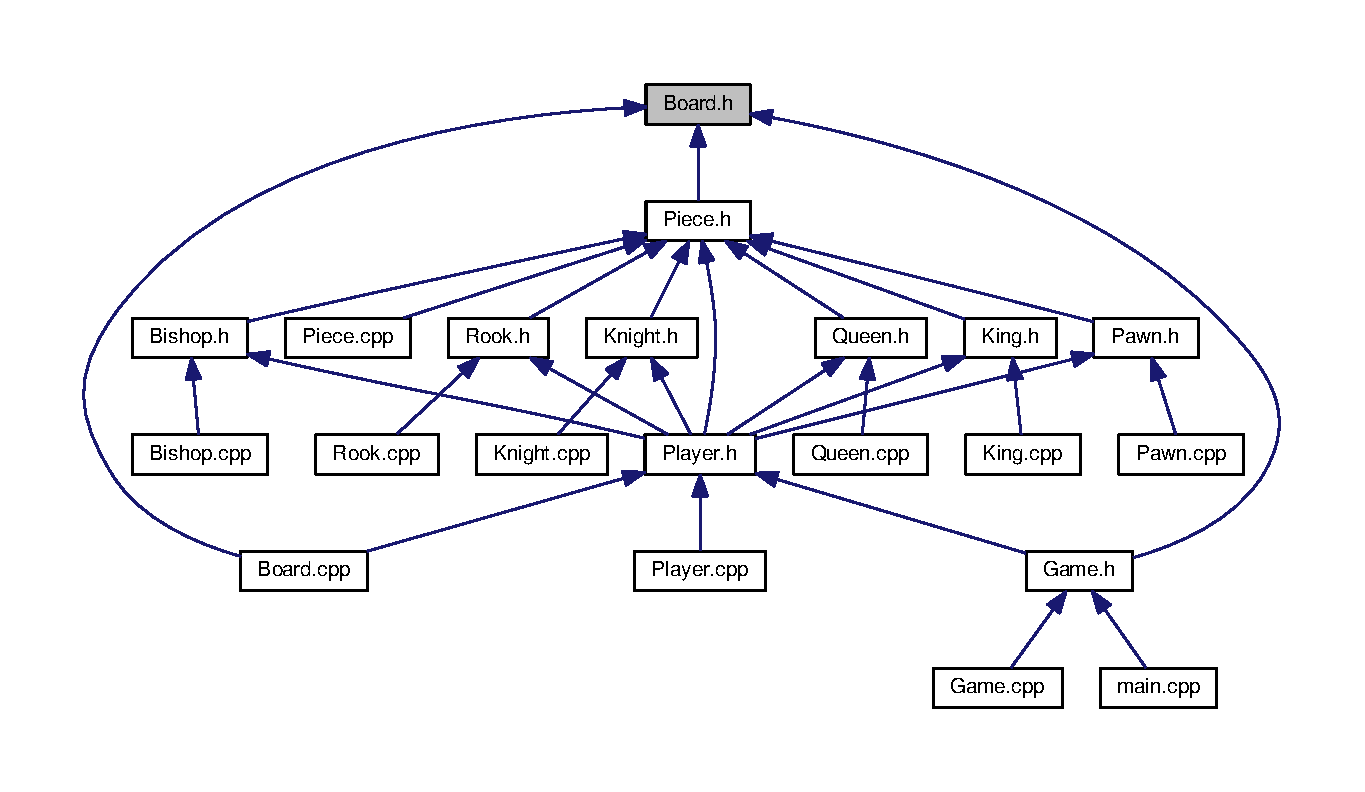
\includegraphics[width=350pt]{_board_8h__dep__incl}
\end{center}
\end{figure}
\subsection*{Classes}
\begin{DoxyCompactItemize}
\item 
class \hyperlink{class_board}{Board}
\end{DoxyCompactItemize}

\hypertarget{_case_8cpp}{}\section{Case.\+cpp File Reference}
\label{_case_8cpp}\index{Case.\+cpp@{Case.\+cpp}}
{\ttfamily \#include \char`\"{}Case.\+h\char`\"{}}\\*
Include dependency graph for Case.\+cpp\+:
\nopagebreak
\begin{figure}[H]
\begin{center}
\leavevmode
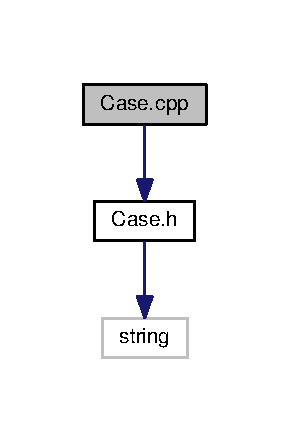
\includegraphics[width=139pt]{_case_8cpp__incl}
\end{center}
\end{figure}

\hypertarget{_case_8h}{}\section{Case.\+h File Reference}
\label{_case_8h}\index{Case.\+h@{Case.\+h}}
{\ttfamily \#include $<$string$>$}\\*
Include dependency graph for Case.\+h\+:\nopagebreak
\begin{figure}[H]
\begin{center}
\leavevmode
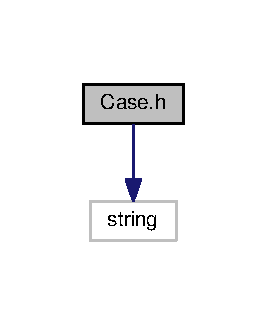
\includegraphics[width=128pt]{_case_8h__incl}
\end{center}
\end{figure}
This graph shows which files directly or indirectly include this file\+:\nopagebreak
\begin{figure}[H]
\begin{center}
\leavevmode
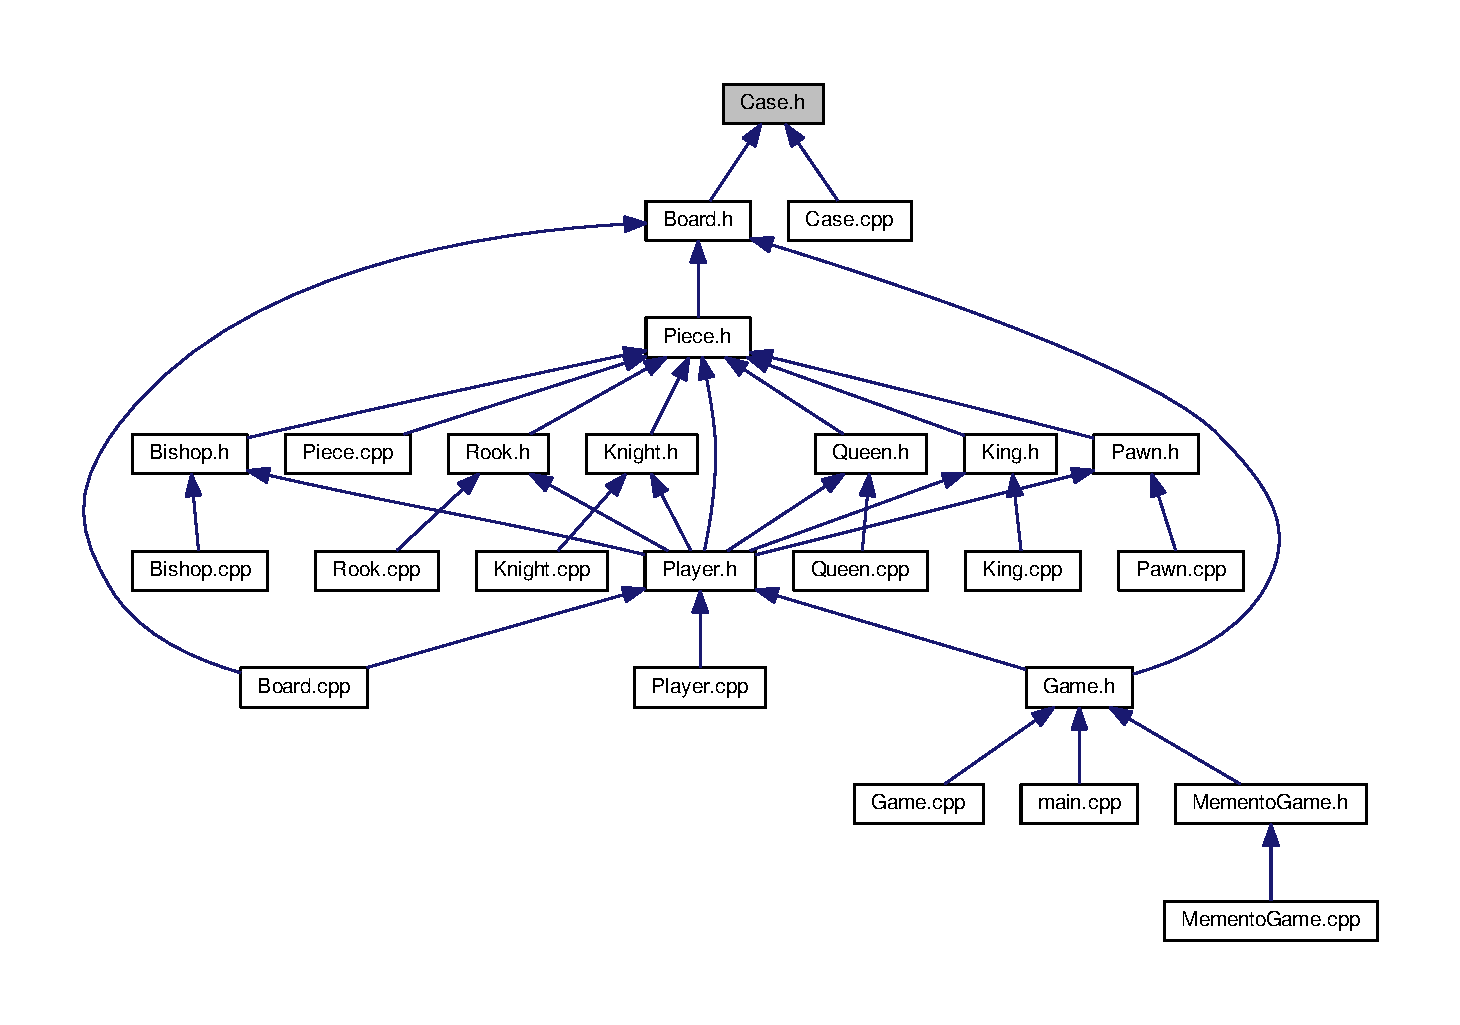
\includegraphics[width=350pt]{_case_8h__dep__incl}
\end{center}
\end{figure}
\subsection*{Classes}
\begin{DoxyCompactItemize}
\item 
class \hyperlink{class_case}{Case}
\end{DoxyCompactItemize}

\hypertarget{_coordinate_8cpp}{}\section{Coordinate.\+cpp File Reference}
\label{_coordinate_8cpp}\index{Coordinate.\+cpp@{Coordinate.\+cpp}}
{\ttfamily \#include \char`\"{}Coordinate.\+h\char`\"{}}\\*
Include dependency graph for Coordinate.\+cpp\+:\nopagebreak
\begin{figure}[H]
\begin{center}
\leavevmode
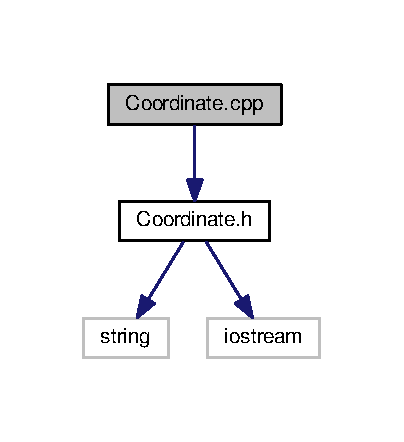
\includegraphics[width=194pt]{_coordinate_8cpp__incl}
\end{center}
\end{figure}

\hypertarget{_coordinate_8h}{}\section{Coordinate.\+h File Reference}
\label{_coordinate_8h}\index{Coordinate.\+h@{Coordinate.\+h}}
{\ttfamily \#include $<$string$>$}\\*
{\ttfamily \#include $<$iostream$>$}\\*
Include dependency graph for Coordinate.\+h\+:
\nopagebreak
\begin{figure}[H]
\begin{center}
\leavevmode
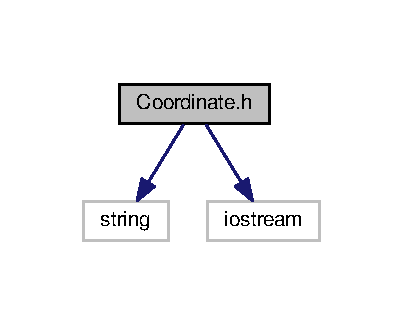
\includegraphics[width=194pt]{_coordinate_8h__incl}
\end{center}
\end{figure}
This graph shows which files directly or indirectly include this file\+:
\nopagebreak
\begin{figure}[H]
\begin{center}
\leavevmode
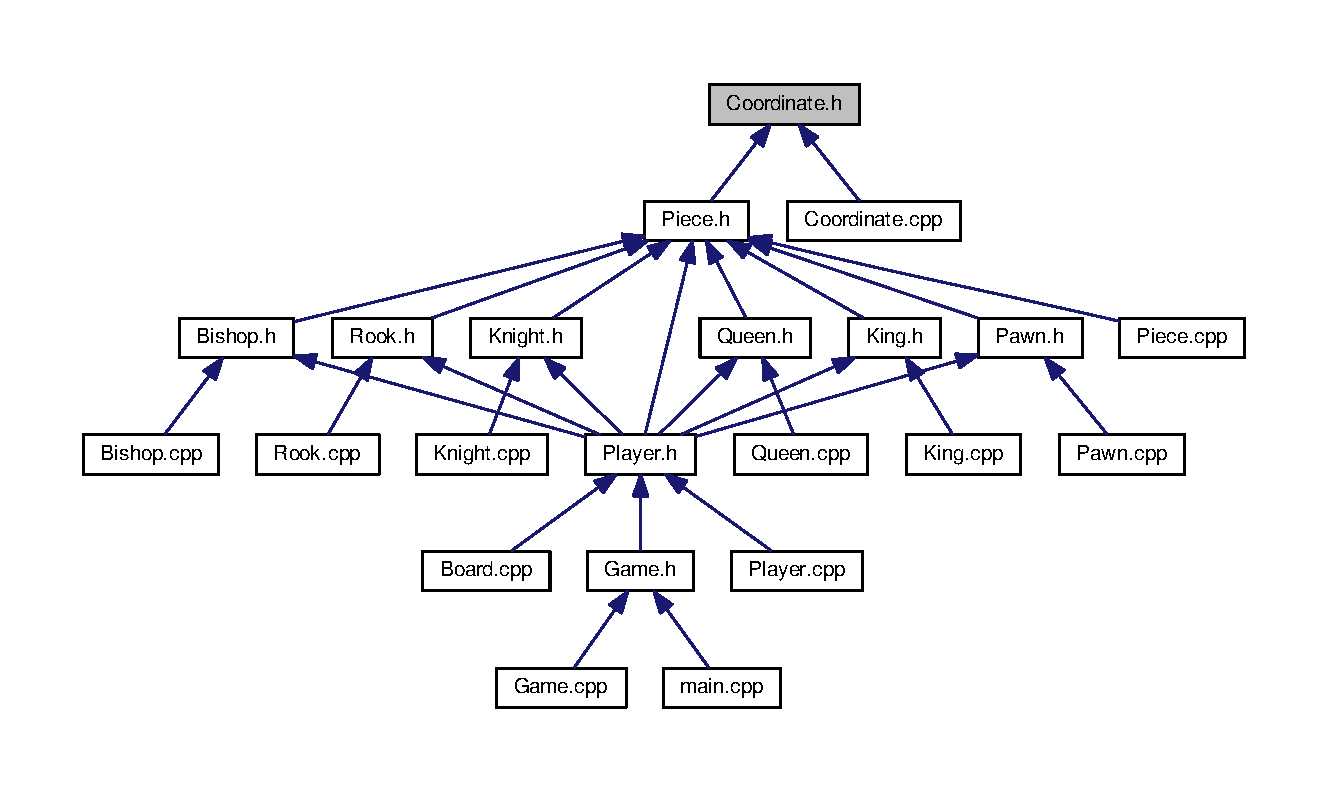
\includegraphics[width=350pt]{_coordinate_8h__dep__incl}
\end{center}
\end{figure}
\subsection*{Classes}
\begin{DoxyCompactItemize}
\item 
class \hyperlink{class_coordinate}{Coordinate}
\end{DoxyCompactItemize}

\hypertarget{_game_8cpp}{}\section{Game.\+cpp File Reference}
\label{_game_8cpp}\index{Game.\+cpp@{Game.\+cpp}}
{\ttfamily \#include \char`\"{}Game.\+h\char`\"{}}\\*
Include dependency graph for Game.\+cpp\+:
\nopagebreak
\begin{figure}[H]
\begin{center}
\leavevmode
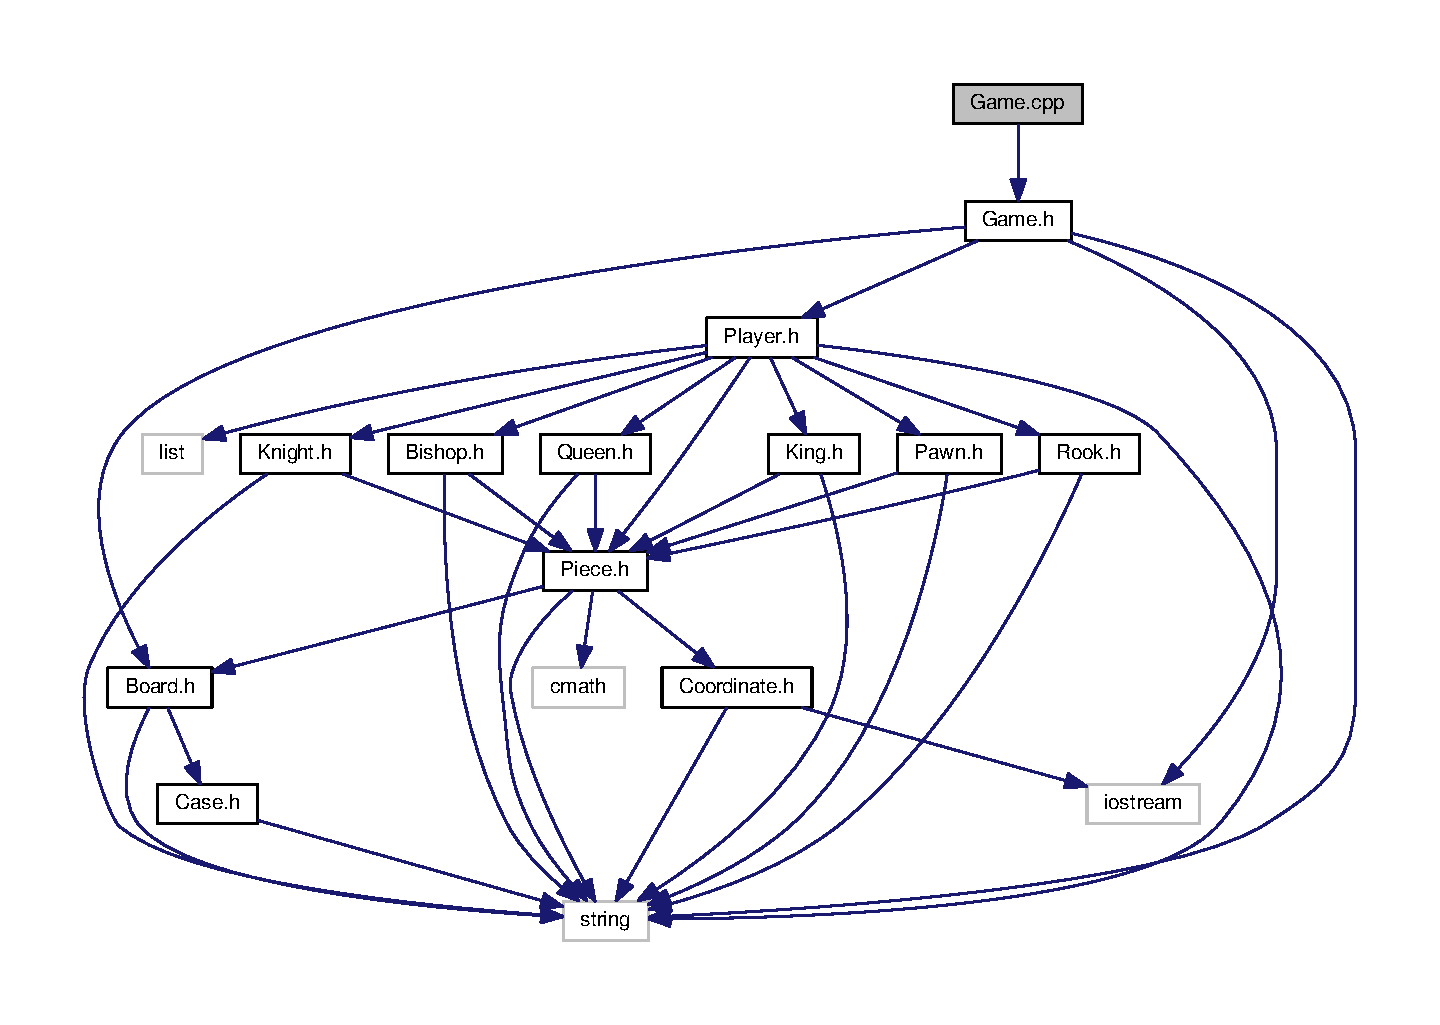
\includegraphics[width=350pt]{_game_8cpp__incl}
\end{center}
\end{figure}

\hypertarget{_game_8h}{}\section{Game.\+h File Reference}
\label{_game_8h}\index{Game.\+h@{Game.\+h}}
{\ttfamily \#include $<$string$>$}\\*
{\ttfamily \#include \char`\"{}Board.\+h\char`\"{}}\\*
{\ttfamily \#include \char`\"{}Player.\+h\char`\"{}}\\*
{\ttfamily \#include $<$iostream$>$}\\*
Include dependency graph for Game.\+h\+:
\nopagebreak
\begin{figure}[H]
\begin{center}
\leavevmode
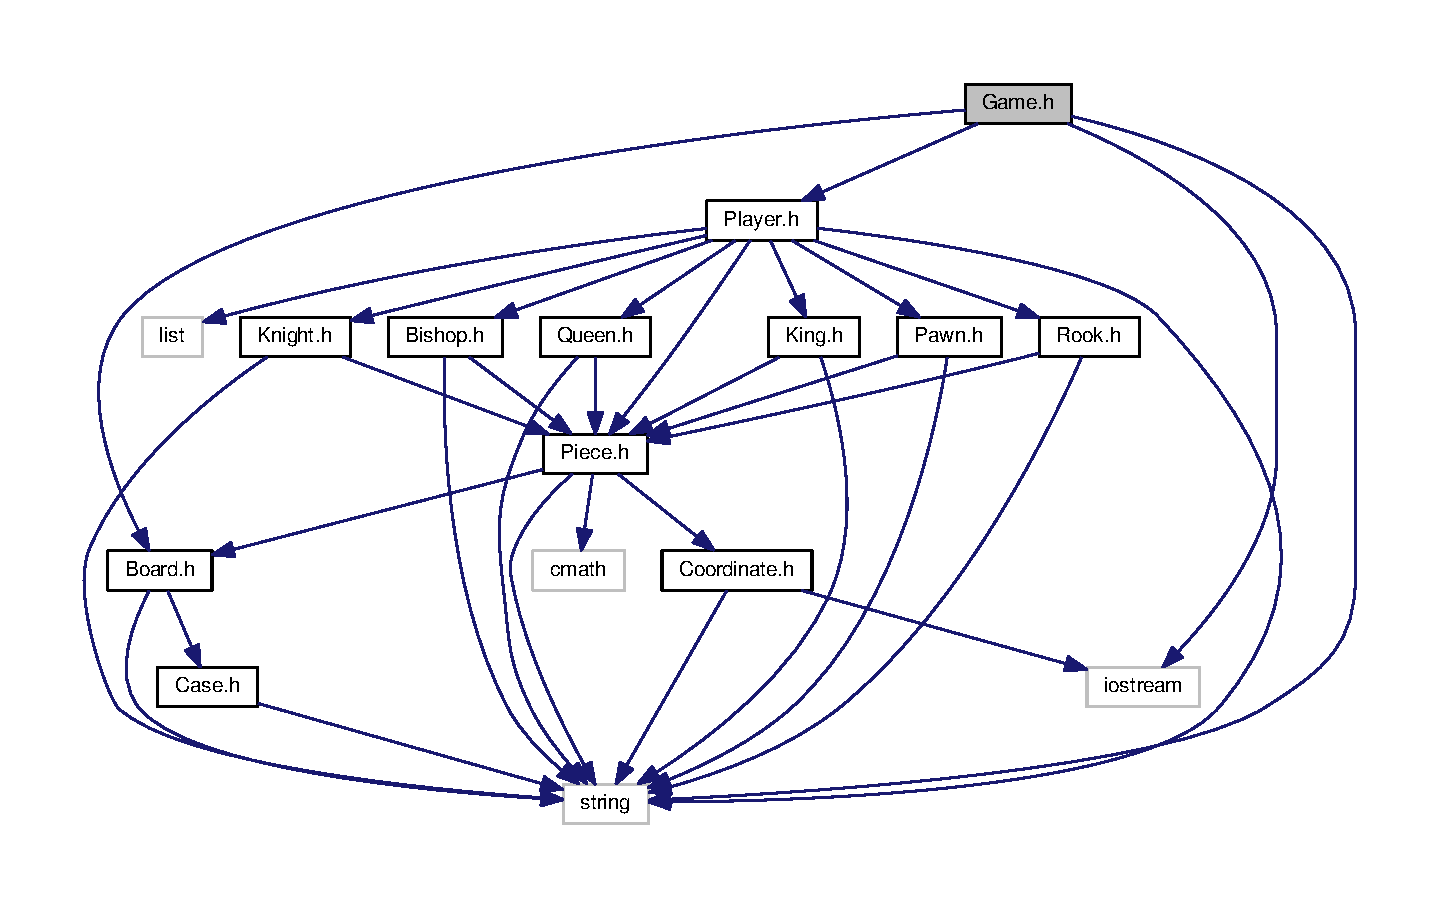
\includegraphics[width=350pt]{_game_8h__incl}
\end{center}
\end{figure}
This graph shows which files directly or indirectly include this file\+:
\nopagebreak
\begin{figure}[H]
\begin{center}
\leavevmode
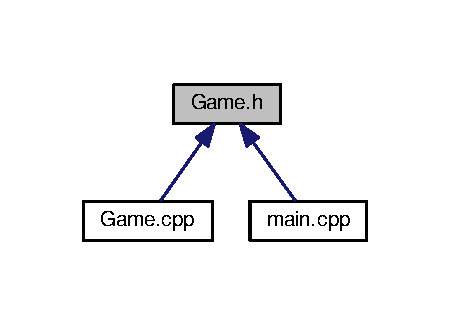
\includegraphics[width=331pt]{_game_8h__dep__incl}
\end{center}
\end{figure}
\subsection*{Classes}
\begin{DoxyCompactItemize}
\item 
class \hyperlink{class_game}{Game}
\end{DoxyCompactItemize}

\hypertarget{_king_8cpp}{}\section{King.\+cpp File Reference}
\label{_king_8cpp}\index{King.\+cpp@{King.\+cpp}}
{\ttfamily \#include \char`\"{}King.\+h\char`\"{}}\\*
Include dependency graph for King.\+cpp\+:
\nopagebreak
\begin{figure}[H]
\begin{center}
\leavevmode
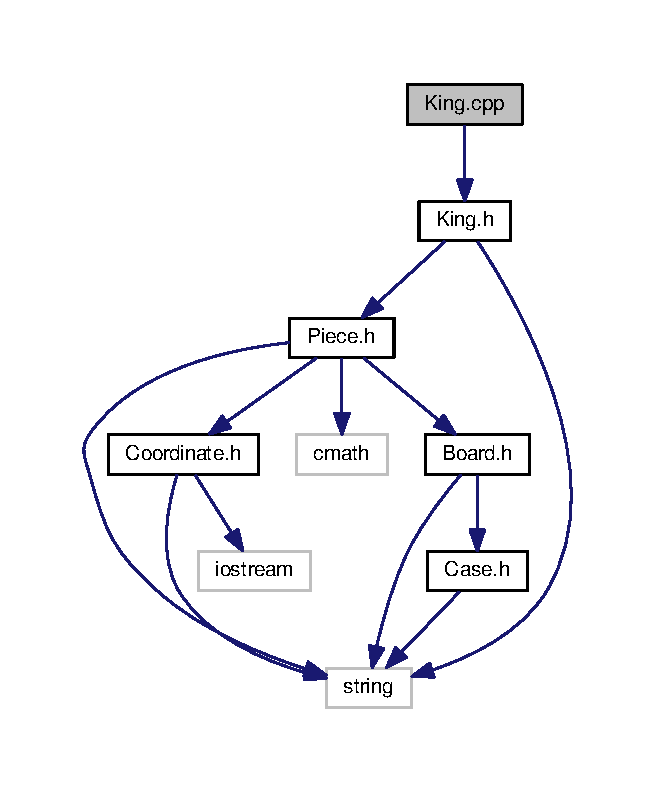
\includegraphics[width=314pt]{_king_8cpp__incl}
\end{center}
\end{figure}

\hypertarget{_king_8h}{}\section{King.\+h File Reference}
\label{_king_8h}\index{King.\+h@{King.\+h}}
{\ttfamily \#include \char`\"{}Piece.\+h\char`\"{}}\\*
{\ttfamily \#include $<$string$>$}\\*
Include dependency graph for King.\+h\+:\nopagebreak
\begin{figure}[H]
\begin{center}
\leavevmode
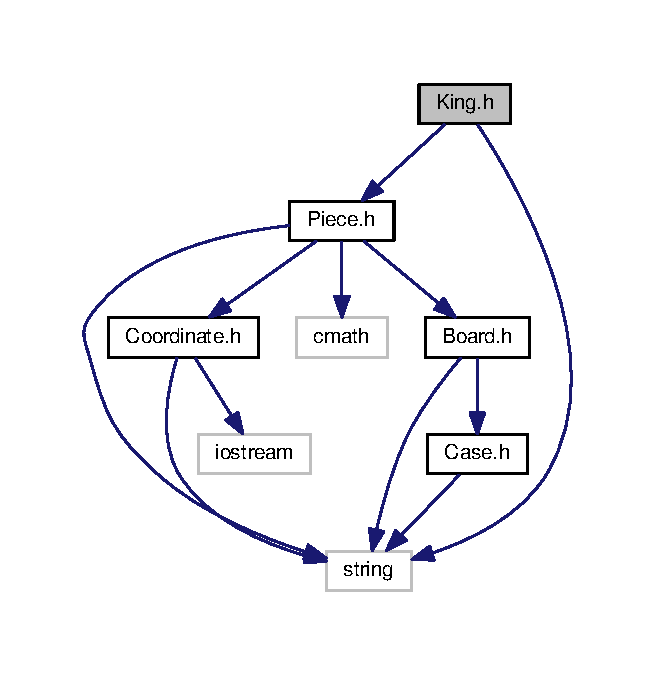
\includegraphics[width=314pt]{_king_8h__incl}
\end{center}
\end{figure}
This graph shows which files directly or indirectly include this file\+:\nopagebreak
\begin{figure}[H]
\begin{center}
\leavevmode
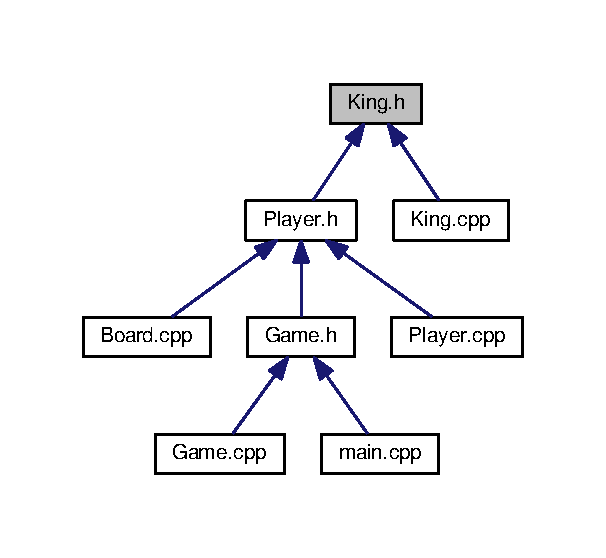
\includegraphics[width=291pt]{_king_8h__dep__incl}
\end{center}
\end{figure}
\subsection*{Classes}
\begin{DoxyCompactItemize}
\item 
class \hyperlink{class_king}{King}
\end{DoxyCompactItemize}

\hypertarget{_knight_8cpp}{}\section{Knight.\+cpp File Reference}
\label{_knight_8cpp}\index{Knight.\+cpp@{Knight.\+cpp}}
{\ttfamily \#include \char`\"{}Knight.\+h\char`\"{}}\\*
Include dependency graph for Knight.\+cpp\+:\nopagebreak
\begin{figure}[H]
\begin{center}
\leavevmode
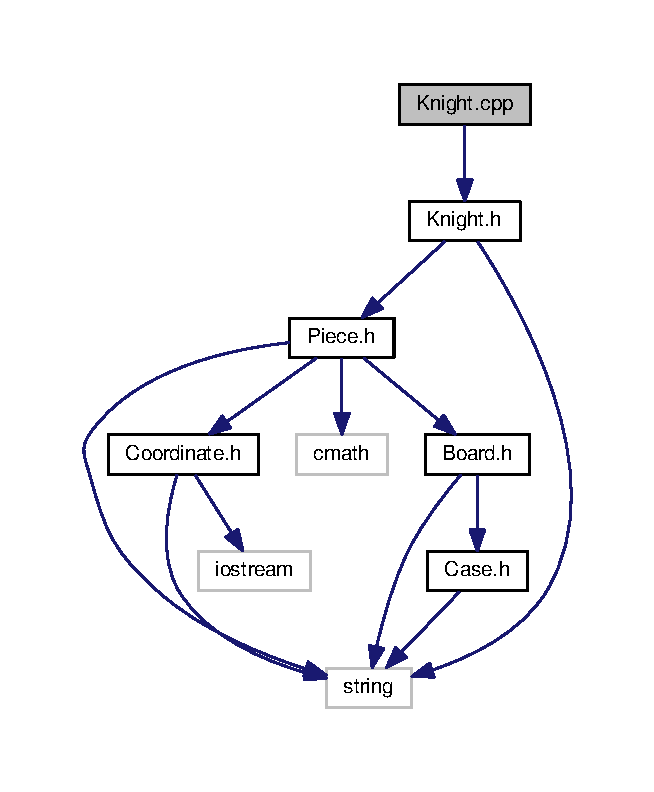
\includegraphics[width=314pt]{_knight_8cpp__incl}
\end{center}
\end{figure}

\hypertarget{_knight_8h}{}\section{Knight.\+h File Reference}
\label{_knight_8h}\index{Knight.\+h@{Knight.\+h}}
{\ttfamily \#include \char`\"{}Piece.\+h\char`\"{}}\\*
{\ttfamily \#include $<$string$>$}\\*
Include dependency graph for Knight.\+h\+:\nopagebreak
\begin{figure}[H]
\begin{center}
\leavevmode
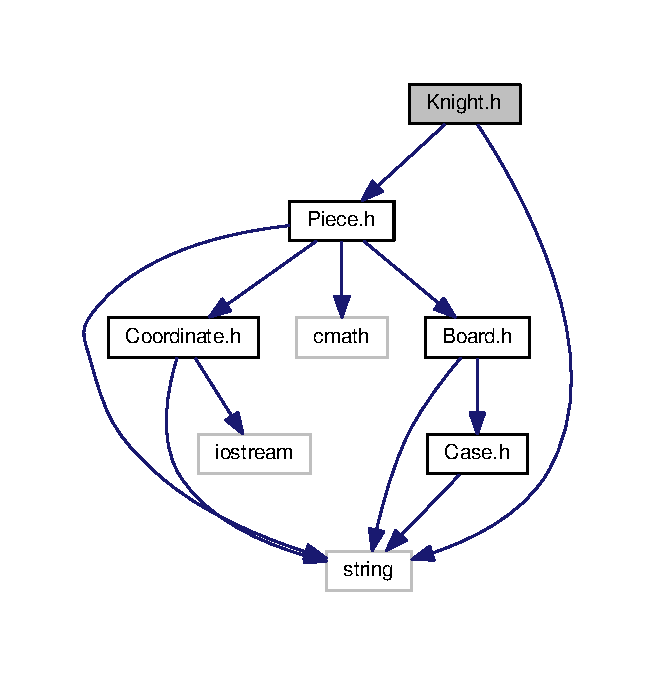
\includegraphics[width=314pt]{_knight_8h__incl}
\end{center}
\end{figure}
This graph shows which files directly or indirectly include this file\+:\nopagebreak
\begin{figure}[H]
\begin{center}
\leavevmode
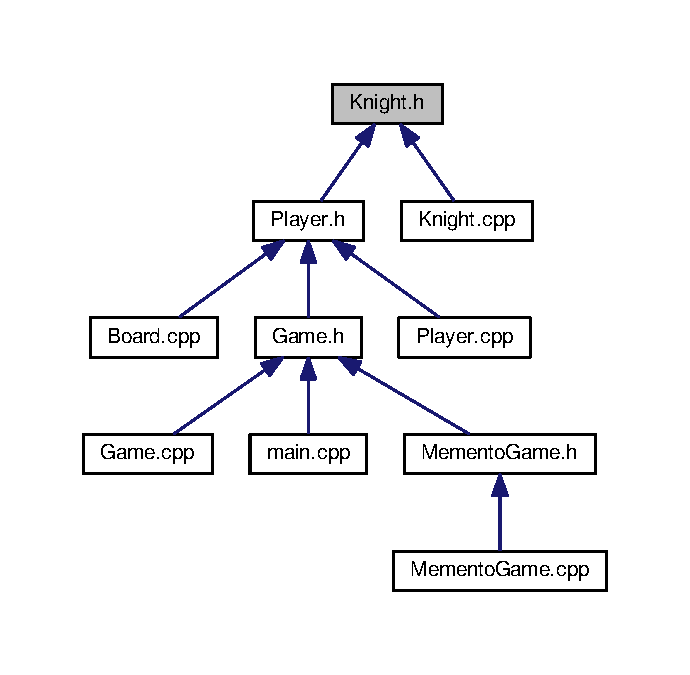
\includegraphics[width=292pt]{_knight_8h__dep__incl}
\end{center}
\end{figure}
\subsection*{Classes}
\begin{DoxyCompactItemize}
\item 
class \hyperlink{class_knight}{Knight}
\end{DoxyCompactItemize}

\hypertarget{main_8cpp}{}\section{main.\+cpp File Reference}
\label{main_8cpp}\index{main.\+cpp@{main.\+cpp}}
{\ttfamily \#include $<$Q\+Gui\+Application$>$}\\*
{\ttfamily \#include $<$Q\+Qml\+Application\+Engine$>$}\\*
{\ttfamily \#include \char`\"{}Game.\+h\char`\"{}}\\*
Include dependency graph for main.\+cpp\+:
\nopagebreak
\begin{figure}[H]
\begin{center}
\leavevmode
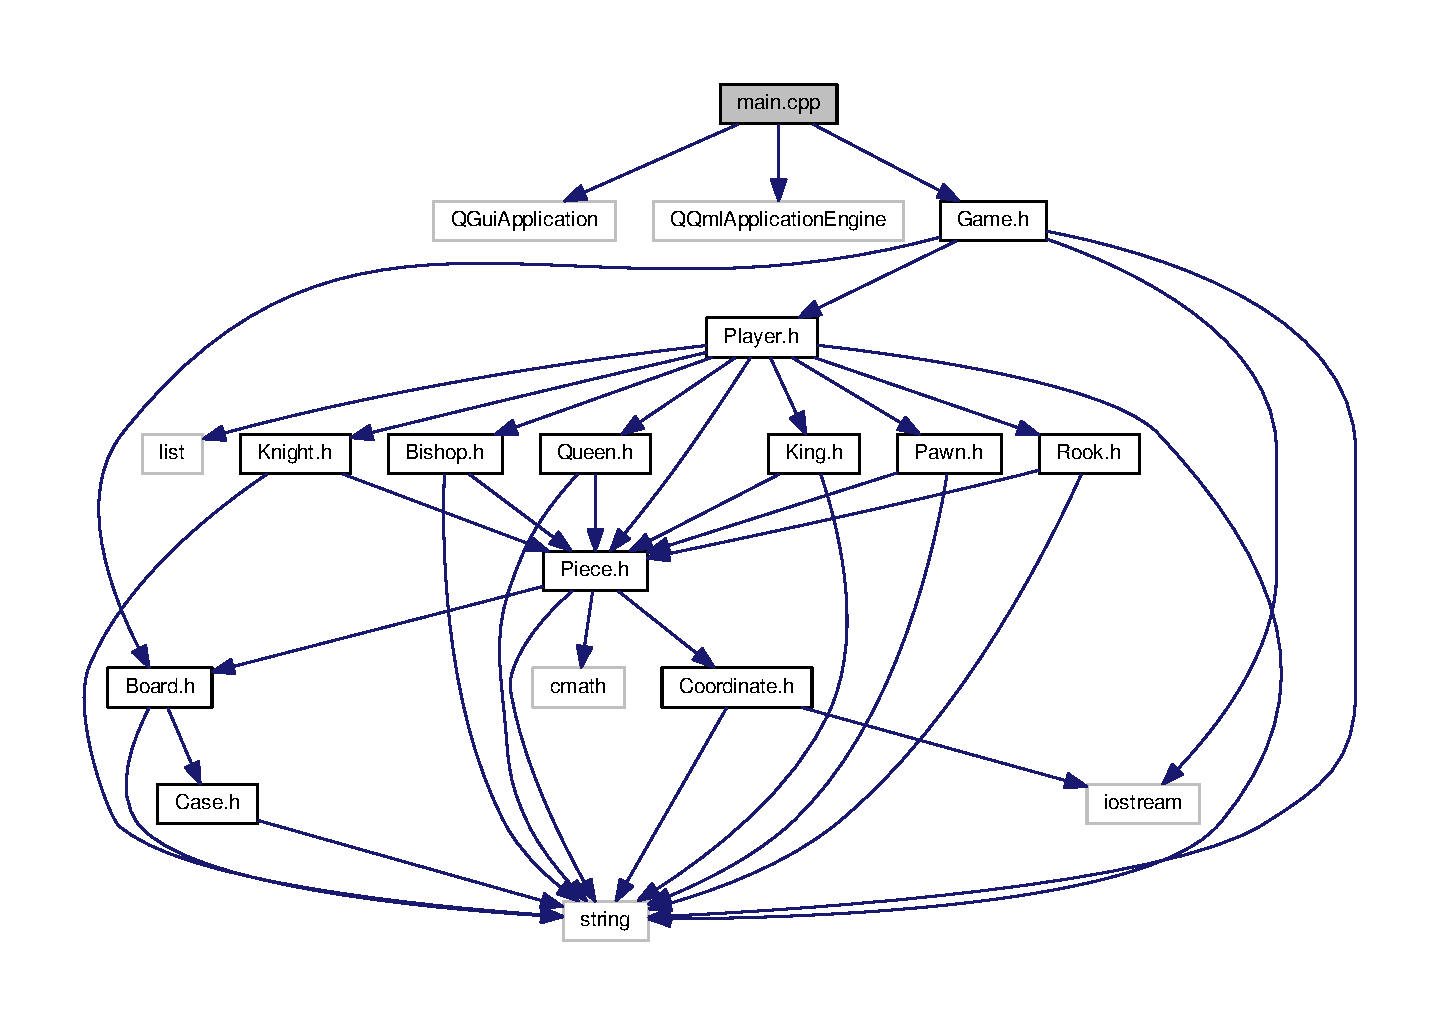
\includegraphics[width=350pt]{main_8cpp__incl}
\end{center}
\end{figure}
\subsection*{Functions}
\begin{DoxyCompactItemize}
\item 
int \hyperlink{main_8cpp_a0ddf1224851353fc92bfbff6f499fa97}{main} (int argc, char $\ast$argv\mbox{[}$\,$\mbox{]})
\end{DoxyCompactItemize}


\subsection{Function Documentation}
\index{main.\+cpp@{main.\+cpp}!main@{main}}
\index{main@{main}!main.\+cpp@{main.\+cpp}}
\subsubsection[{\texorpdfstring{main(int argc, char $\ast$argv[])}{main(int argc, char *argv[])}}]{\setlength{\rightskip}{0pt plus 5cm}int main (
\begin{DoxyParamCaption}
\item[{int}]{argc, }
\item[{char $\ast$}]{argv\mbox{[}$\,$\mbox{]}}
\end{DoxyParamCaption}
)}\hypertarget{main_8cpp_a0ddf1224851353fc92bfbff6f499fa97}{}\label{main_8cpp_a0ddf1224851353fc92bfbff6f499fa97}

\hypertarget{_memento_game_8cpp}{}\section{Memento\+Game.\+cpp File Reference}
\label{_memento_game_8cpp}\index{Memento\+Game.\+cpp@{Memento\+Game.\+cpp}}
{\ttfamily \#include \char`\"{}Memento\+Game.\+h\char`\"{}}\\*
Include dependency graph for Memento\+Game.\+cpp\+:
\nopagebreak
\begin{figure}[H]
\begin{center}
\leavevmode
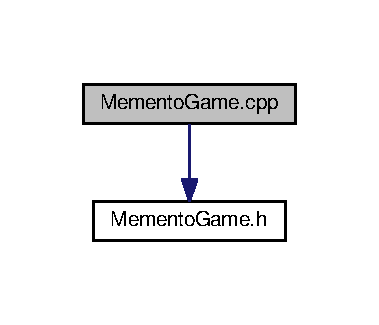
\includegraphics[width=350pt]{_memento_game_8cpp__incl}
\end{center}
\end{figure}

\hypertarget{_memento_game_8h}{}\section{Memento\+Game.\+h File Reference}
\label{_memento_game_8h}\index{Memento\+Game.\+h@{Memento\+Game.\+h}}
{\ttfamily \#include \char`\"{}Game.\+h\char`\"{}}\\*
{\ttfamily \#include $<$list$>$}\\*
Include dependency graph for Memento\+Game.\+h\+:
\nopagebreak
\begin{figure}[H]
\begin{center}
\leavevmode
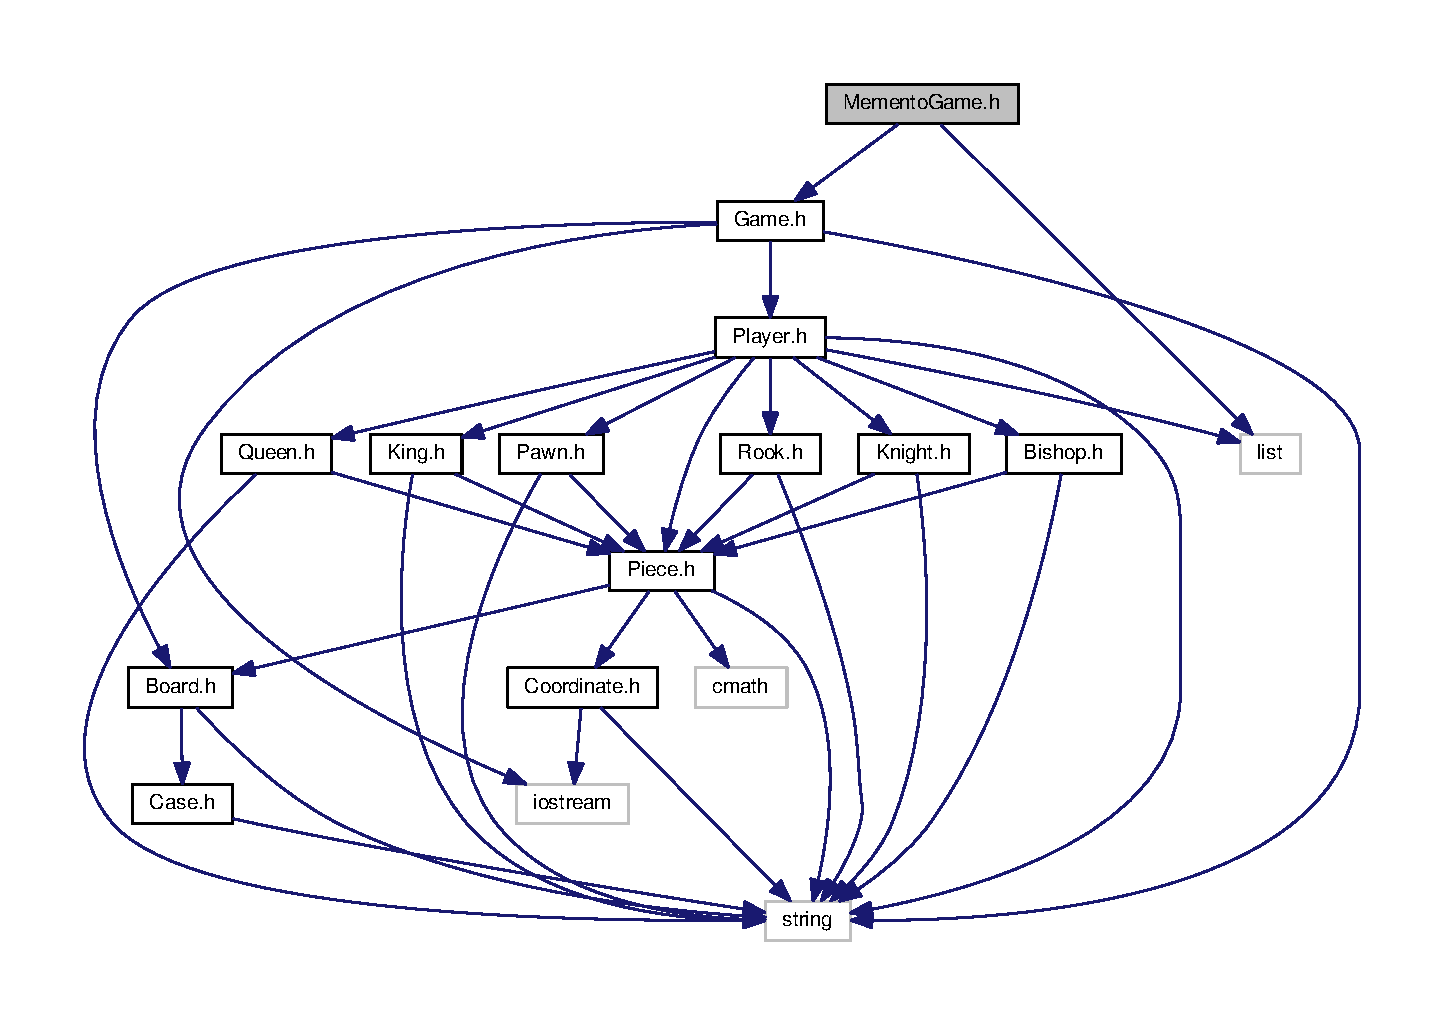
\includegraphics[width=350pt]{_memento_game_8h__incl}
\end{center}
\end{figure}
This graph shows which files directly or indirectly include this file\+:
\nopagebreak
\begin{figure}[H]
\begin{center}
\leavevmode
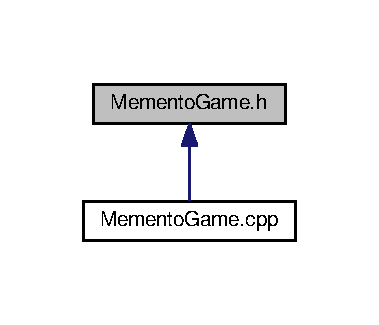
\includegraphics[width=182pt]{_memento_game_8h__dep__incl}
\end{center}
\end{figure}
\subsection*{Classes}
\begin{DoxyCompactItemize}
\item 
class \hyperlink{class_memento_game}{Memento\+Game}
\end{DoxyCompactItemize}

\hypertarget{_pawn_8cpp}{}\section{Pawn.\+cpp File Reference}
\label{_pawn_8cpp}\index{Pawn.\+cpp@{Pawn.\+cpp}}
{\ttfamily \#include \char`\"{}Pawn.\+h\char`\"{}}\\*
Include dependency graph for Pawn.\+cpp\+:\nopagebreak
\begin{figure}[H]
\begin{center}
\leavevmode
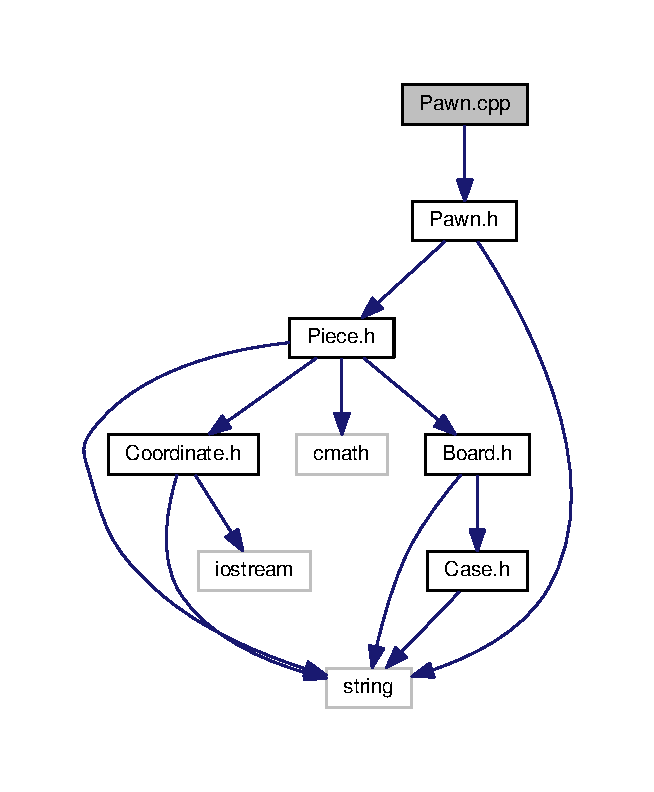
\includegraphics[width=314pt]{_pawn_8cpp__incl}
\end{center}
\end{figure}

\hypertarget{_pawn_8h}{}\section{Pawn.\+h File Reference}
\label{_pawn_8h}\index{Pawn.\+h@{Pawn.\+h}}
{\ttfamily \#include \char`\"{}Piece.\+h\char`\"{}}\\*
{\ttfamily \#include $<$string$>$}\\*
Include dependency graph for Pawn.\+h\+:\nopagebreak
\begin{figure}[H]
\begin{center}
\leavevmode
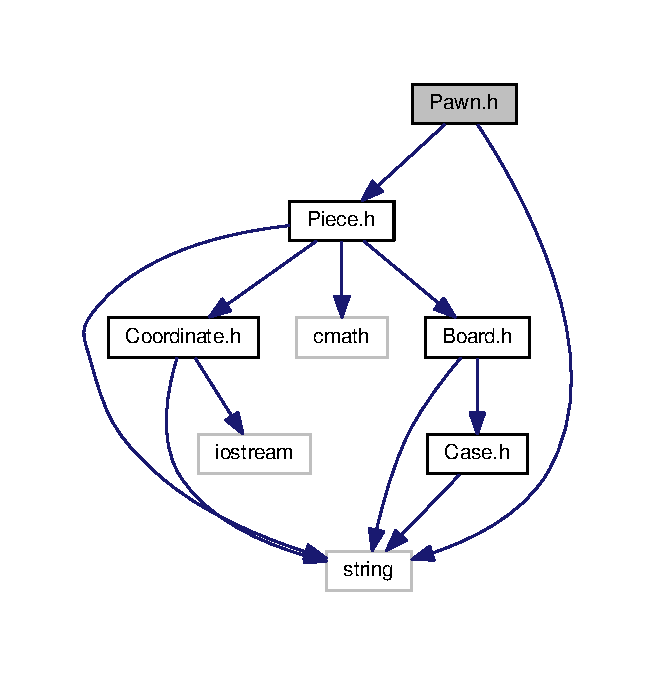
\includegraphics[width=314pt]{_pawn_8h__incl}
\end{center}
\end{figure}
This graph shows which files directly or indirectly include this file\+:\nopagebreak
\begin{figure}[H]
\begin{center}
\leavevmode
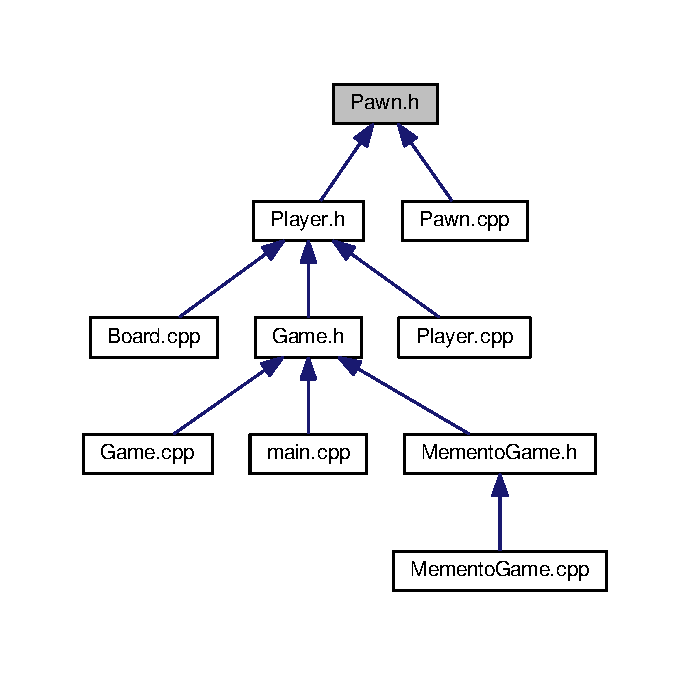
\includegraphics[width=291pt]{_pawn_8h__dep__incl}
\end{center}
\end{figure}
\subsection*{Classes}
\begin{DoxyCompactItemize}
\item 
class \hyperlink{class_pawn}{Pawn}
\end{DoxyCompactItemize}

\hypertarget{_piece_8cpp}{}\section{Piece.\+cpp File Reference}
\label{_piece_8cpp}\index{Piece.\+cpp@{Piece.\+cpp}}
{\ttfamily \#include \char`\"{}Piece.\+h\char`\"{}}\\*
Include dependency graph for Piece.\+cpp\+:
\nopagebreak
\begin{figure}[H]
\begin{center}
\leavevmode
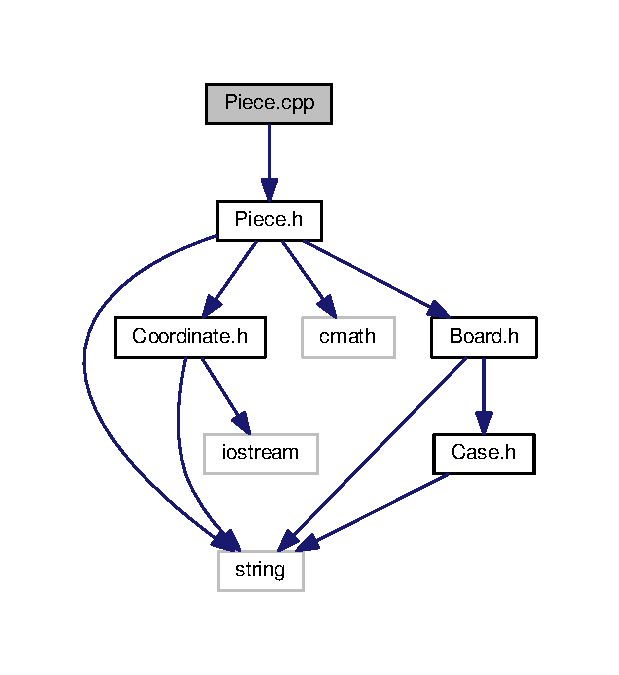
\includegraphics[width=297pt]{_piece_8cpp__incl}
\end{center}
\end{figure}

\hypertarget{_piece_8h}{}\section{Piece.\+h File Reference}
\label{_piece_8h}\index{Piece.\+h@{Piece.\+h}}
{\ttfamily \#include $<$string$>$}\\*
{\ttfamily \#include \char`\"{}Coordinate.\+h\char`\"{}}\\*
{\ttfamily \#include $<$cmath$>$}\\*
{\ttfamily \#include \char`\"{}Board.\+h\char`\"{}}\\*
Include dependency graph for Piece.\+h\+:\nopagebreak
\begin{figure}[H]
\begin{center}
\leavevmode
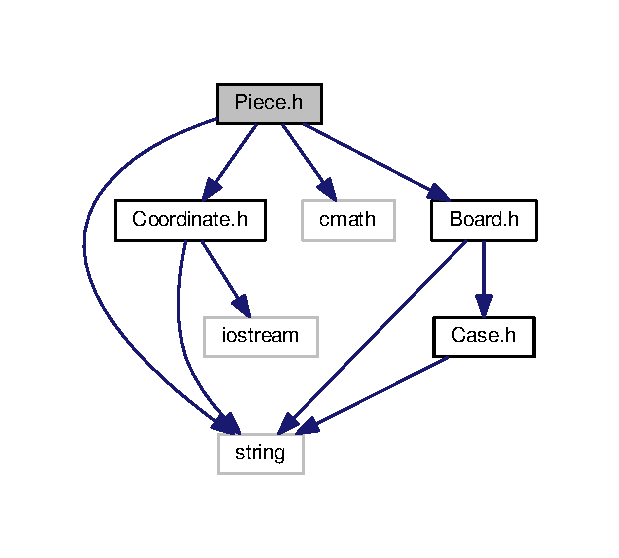
\includegraphics[width=297pt]{_piece_8h__incl}
\end{center}
\end{figure}
This graph shows which files directly or indirectly include this file\+:\nopagebreak
\begin{figure}[H]
\begin{center}
\leavevmode
\includegraphics[width=350pt]{_piece_8h__dep__incl}
\end{center}
\end{figure}
\subsection*{Classes}
\begin{DoxyCompactItemize}
\item 
class \hyperlink{class_piece}{Piece}
\end{DoxyCompactItemize}

\hypertarget{_player_8cpp}{}\section{Player.\+cpp File Reference}
\label{_player_8cpp}\index{Player.\+cpp@{Player.\+cpp}}
{\ttfamily \#include \char`\"{}Player.\+h\char`\"{}}\\*
Include dependency graph for Player.\+cpp\+:\nopagebreak
\begin{figure}[H]
\begin{center}
\leavevmode
\includegraphics[width=350pt]{_player_8cpp__incl}
\end{center}
\end{figure}

\hypertarget{_player_8h}{}\section{Player.\+h File Reference}
\label{_player_8h}\index{Player.\+h@{Player.\+h}}
{\ttfamily \#include $<$string$>$}\\*
{\ttfamily \#include $<$list$>$}\\*
{\ttfamily \#include \char`\"{}Piece.\+h\char`\"{}}\\*
{\ttfamily \#include \char`\"{}Rook.\+h\char`\"{}}\\*
{\ttfamily \#include \char`\"{}Knight.\+h\char`\"{}}\\*
{\ttfamily \#include \char`\"{}Bishop.\+h\char`\"{}}\\*
{\ttfamily \#include \char`\"{}Queen.\+h\char`\"{}}\\*
{\ttfamily \#include \char`\"{}King.\+h\char`\"{}}\\*
{\ttfamily \#include \char`\"{}Pawn.\+h\char`\"{}}\\*
Include dependency graph for Player.\+h\+:\nopagebreak
\begin{figure}[H]
\begin{center}
\leavevmode
\includegraphics[width=350pt]{_player_8h__incl}
\end{center}
\end{figure}
This graph shows which files directly or indirectly include this file\+:\nopagebreak
\begin{figure}[H]
\begin{center}
\leavevmode
\includegraphics[width=291pt]{_player_8h__dep__incl}
\end{center}
\end{figure}
\subsection*{Classes}
\begin{DoxyCompactItemize}
\item 
class \hyperlink{class_player}{Player}
\end{DoxyCompactItemize}

\hypertarget{_queen_8cpp}{}\section{Queen.\+cpp File Reference}
\label{_queen_8cpp}\index{Queen.\+cpp@{Queen.\+cpp}}
{\ttfamily \#include \char`\"{}Queen.\+h\char`\"{}}\\*
Include dependency graph for Queen.\+cpp\+:
\nopagebreak
\begin{figure}[H]
\begin{center}
\leavevmode
\includegraphics[width=314pt]{_queen_8cpp__incl}
\end{center}
\end{figure}

\hypertarget{_queen_8h}{}\section{Queen.\+h File Reference}
\label{_queen_8h}\index{Queen.\+h@{Queen.\+h}}
{\ttfamily \#include \char`\"{}Piece.\+h\char`\"{}}\\*
{\ttfamily \#include $<$string$>$}\\*
Include dependency graph for Queen.\+h\+:\nopagebreak
\begin{figure}[H]
\begin{center}
\leavevmode
\includegraphics[width=314pt]{_queen_8h__incl}
\end{center}
\end{figure}
This graph shows which files directly or indirectly include this file\+:\nopagebreak
\begin{figure}[H]
\begin{center}
\leavevmode
\includegraphics[width=294pt]{_queen_8h__dep__incl}
\end{center}
\end{figure}
\subsection*{Classes}
\begin{DoxyCompactItemize}
\item 
class \hyperlink{class_queen}{Queen}
\end{DoxyCompactItemize}

\hypertarget{_r_e_a_d_m_e_8md}{}\section{R\+E\+A\+D\+M\+E.\+md File Reference}
\label{_r_e_a_d_m_e_8md}\index{R\+E\+A\+D\+M\+E.\+md@{R\+E\+A\+D\+M\+E.\+md}}

\hypertarget{_rook_8cpp}{}\section{Rook.\+cpp File Reference}
\label{_rook_8cpp}\index{Rook.\+cpp@{Rook.\+cpp}}
{\ttfamily \#include \char`\"{}Rook.\+h\char`\"{}}\\*
Include dependency graph for Rook.\+cpp\+:
\nopagebreak
\begin{figure}[H]
\begin{center}
\leavevmode
\includegraphics[width=314pt]{_rook_8cpp__incl}
\end{center}
\end{figure}

\hypertarget{_rook_8h}{}\section{Rook.\+h File Reference}
\label{_rook_8h}\index{Rook.\+h@{Rook.\+h}}
{\ttfamily \#include \char`\"{}Piece.\+h\char`\"{}}\\*
{\ttfamily \#include $<$string$>$}\\*
Include dependency graph for Rook.\+h\+:
\nopagebreak
\begin{figure}[H]
\begin{center}
\leavevmode
\includegraphics[width=314pt]{_rook_8h__incl}
\end{center}
\end{figure}
This graph shows which files directly or indirectly include this file\+:
\nopagebreak
\begin{figure}[H]
\begin{center}
\leavevmode
\includegraphics[width=331pt]{_rook_8h__dep__incl}
\end{center}
\end{figure}
\subsection*{Classes}
\begin{DoxyCompactItemize}
\item 
class \hyperlink{class_rook}{Rook}
\end{DoxyCompactItemize}

%--- End generated contents ---

% Index
\backmatter
\newpage
\phantomsection
\clearemptydoublepage
\addcontentsline{toc}{chapter}{Index}
\printindex

\end{document}
